% ============================================================
% FeatureScalpel: Project Report (LaTeX source), revised October 2026
% Compile with: pdflatex Reportmain.tex  (run twice for TOC / LoF / LoT)
% Required folder: figures/ next to this file, holding (a) the 20 new figures (fig_*.png, gd_*.png), written by
%   tools/make_report_figures.py and tools/report_diagrams.py in the project repository, and (b) these 13 figures of the
%   first version of the report, which are NOT regenerated: mbcet_logo, delta, dfd0, dfd1, strategy, decay, topk,
%   hybrid, layer, passes, gpu, ui_app, ui_bench. (fig_elig_v2, fig_arch_v2 and fig_algo_v2 replace the old elig, arch and algo.)
% Red [TODO: ...] marks are items only the authors can fill in; search for "TODO".
% ============================================================
\documentclass[12pt,a4paper]{report}

\usepackage[utf8]{inputenc}
\usepackage[T1]{fontenc}
\usepackage{mathptmx}                 % Times font, as in the sample report
\usepackage{courier}                  % scalable monospace for code
\usepackage{amsmath,amssymb}
\usepackage[a4paper,top=1in,bottom=1in,left=1.18in,right=0.875in]{geometry}
\usepackage{setspace}
\usepackage{graphicx}
\usepackage{float}
\usepackage{array}
\usepackage{longtable}
\usepackage{caption}
\usepackage{enumitem}
\usepackage{listings}
\usepackage{xcolor}
\usepackage{url}
\usepackage{hyperref}                 % boxed links, as in the sample report

\onehalfspacing
\renewcommand{\contentsname}{Table of Contents}
\setlength{\parindent}{1.5em}
\setlength{\emergencystretch}{3em}
\captionsetup{labelsep=colon}
\setlist{itemsep=2pt}
\urlstyle{same}

\lstset{basicstyle=\ttfamily\footnotesize, backgroundcolor=\color[gray]{0.95},
  frame=none, columns=fullflexible, keepspaces=true, showstringspaces=false,
  breaklines=true, aboveskip=6pt, belowskip=10pt}

\newcommand{\projecttitle}{FeatureScalpel: Mechanistic Interpretability And Intervention Of Large Language Models via Sparse Autoencoder}
\newcommand{\todo}[1]{{\color{red}[TODO: #1]}}

\begin{document}

% ======================= COVER PAGE =======================
\begin{titlepage}
\centering
{\LARGE\bfseries \projecttitle\par}
\vspace{1.2cm}
{\Large\bfseries A Main Project Report\par}
\vspace{0.6cm}
{\itshape Submitted to the APJ Abdul Kalam Technological University\par
in partial fulfillment of requirements for the award of degree\par}
\vspace{0.8cm}
{\Large\bfseries Bachelor of Technology\par}
\vspace{0.2cm}
in\par
\vspace{0.2cm}
{\Large\bfseries Computer Science and Engineering(AI)\par}
\vspace{0.2cm}
{\itshape by\par}
\vspace{0.2cm}
{\large\bfseries\scshape Adithyan R S \itshape (B23CS2109)}\par
{\large\bfseries\scshape Alona Biju \itshape (B23CS2113)}\par
{\large\bfseries\scshape Alvin Binu \itshape (B23CS2114)}\par
{\large\bfseries\scshape Darsan M \itshape (B23CS2125)}\par
\vfill
\includegraphics[width=4cm]{figures/mbcet_logo}\par
\vspace{0.8cm}
{\bfseries Department of Computer Science and Engineering\par
Mar Baselios College of Engineering and Technology\par
(Autonomous)\par
Mar Ivanios Vidya Nagar, Nalanchira\par
Thiruvananthapuram--695015\par}
\vspace{0.6cm}
{\bfseries October 2026\par}
\end{titlepage}

% ======================= CERTIFICATE =======================
\thispagestyle{empty}
\begin{center}
{\bfseries DEPARTMENT OF COMPUTER SCIENCE AND ENGINEERING\\
MAR BASELIOS COLLEGE OF ENGINEERING AND TECHNOLOGY\\
(AUTONOMOUS)\\
MAR IVANIOS VIDYA NAGAR, NALANCHIRA\\
THIRUVANANTHAPURAM--695015\par}
\vspace{1cm}
\includegraphics[width=4cm]{figures/mbcet_logo}\par
\vspace{1.2cm}
{\Large\bfseries\scshape Certificate\par}
\end{center}
\vspace{0.4cm}
\noindent\hspace{1.5em}This is to certify that the report entitled \textbf{\projecttitle} submitted by \textbf{Adithyan R S} (KTU Reg No: B23CS2109), \textbf{Alona Biju} (KTU Reg No: B23CS2113), \textbf{Alvin Binu} (KTU Reg No: B23CS2114) and \textbf{Darsan M} (KTU Reg No: B23CS2125) to the APJ Abdul Kalam Technological University in partial fulfillment of the B.Tech.\ degree in Computer Science and Engineering (AI) is a bonafide record of the project work carried out by them under our guidance and supervision. This report in any form has not been submitted to any other University or Institute for any purpose.

\vspace{2.5cm}
\noindent
\begin{minipage}[t]{0.5\textwidth}
\textbf{Ms.\ Poorna B R}\\
(Project Guide)\\
\todo{designation}\\
Department of CSE
\end{minipage}%
\begin{minipage}[t]{0.5\textwidth}
\textbf{Dr. Jisha John}\\
(Head of the Department)\\
Professor\\
Department of CSE
\end{minipage}

\vspace{2.5cm}
\noindent Place: Thiruvananthapuram \hfill Date: \hspace{3cm}
\clearpage

% ======================= DECLARATION =======================
\thispagestyle{empty}
\begin{center}{\LARGE\bfseries Declaration\par}\end{center}
\vspace{1cm}
We hereby declare that the project report entitled \textbf{\projecttitle}, submitted to the APJ Abdul Kalam Technological University in partial fulfillment of the requirements for the award of the degree of Bachelor of Technology in Computer Science and Engineering (AI), is a record of original work carried out by us at the Department of Computer Science and Engineering, Mar Baselios College of Engineering and Technology (Autonomous), Thiruvananthapuram. The experimental results reported here were produced by the system described in this report. Wherever the work of others has been used, it has been duly acknowledged and cited. This report has not been submitted, in whole or in part, to any other University or Institute for the award of any degree or diploma.

\vspace{2.5cm}
\noindent Place: Thiruvananthapuram \hfill \textbf{Adithyan R S} (B23CS2109)\\
Date: \hfill \textbf{Alona Biju} (B23CS2113)\\
\mbox{} \hfill \textbf{Alvin Binu} (B23CS2114)\\
\mbox{} \hfill \textbf{Darsan M} (B23CS2125)
\clearpage

% ======================= FRONT MATTER =======================
\pagenumbering{roman}
\setcounter{page}{1}

\chapter*{\centering Acknowledgement}
\addcontentsline{toc}{chapter}{Acknowledgement}
We express our deepest gratitude to our \textbf{Project Guide} from the Department of Computer Science and Engineering for continuous guidance, critical feedback and technical insight throughout this project. Their advice on experimental rigour and on stating results precisely shaped both the direction and the quality of this work.

We sincerely thank \textbf{Dr. Jisha John}, Head of the Department of Computer Science and Engineering, for academic support, provision of resources and encouragement at every stage of the project.

We acknowledge the open-source communities behind \textbf{PyTorch}, \textbf{TransformerLens}, \textbf{SAELens}, \textbf{Hugging Face} and \textbf{Streamlit}, the author of the pretrained \textbf{gpt2-small-res-jb} sparse autoencoders, and the \textbf{Neuronpedia} project. Without these tools and openly released models, this work would not have been feasible within the project timeframe. We also thank the authors of ROME, whose openly released fact datasets, including CounterFact, formed the basis of the benchmarks.

Finally, we are grateful to our families and friends for their patience and encouragement throughout this endeavour.

\vspace{1cm}
\begin{flushright}\textbf{Adithyan R S}\\ \textbf{Alona Biju}\\ \textbf{Alvin Binu}\\ \textbf{Darsan M}\end{flushright}

\chapter*{\centering Abstract}
\addcontentsline{toc}{chapter}{Abstract}
Language models sometimes rank a correct completion below competing tokens even though they assign it non-trivial probability. Existing corrections either modify model weights permanently, as in ROME and MEMIT, which degrade as edits accumulate, or add external text to the prompt. This project, \textbf{FeatureScalpel}, studies a \textbf{transient, weight-free alternative} for GPT-2 Small: during one forward pass, the residual stream at a chosen layer is edited through the features of a pretrained \textbf{sparse autoencoder (SAE)}, and the edit is discarded when the pass ends.

The report follows the system from single-feature ablation, which corrected 1 and 3 of 22 suppressed facts in its first two versions, to a \textbf{Hybrid Mute \& Boost sweep} (causal feature ranking, a per-feature safety filter, best-so-far tracking and pool refill) and then to \textbf{per-feature gradient descent}, which tunes one multiplier for every candidate feature on the given prompt. On the sweep, drawing candidate features from all prompt positions brought the target to rank 1 on 10 of 13 comparable prompts against 4 of 13 for the last token only, and removing the safety filter lost 10 of 29 successes in a 45-prompt study while relaxing it added at most one prompt. On 300 held-out CounterFact prompts, with the same allowed range of 0 to 3 times per feature, gradient descent reached rank 1 on 271 prompts, against 161 for the wide sweep and 94 for the original sweep settings, with lower same-prompt side effects on 160 of the 161 prompts that both solved and about 5 to 6.5 times less compute time.

Reaching rank 1 proved a weak test. An additive edit that switches on silent features pushed random unrelated words to rank 1 on 20 of 20 prompts, so reachability by steering is not evidence about what a model knows, and the early classification of some facts as absent from the model was withdrawn. Tests on generated text showed a mild increase in repetition and an edit that largely ignores an instruction not to say the target word. No comparison with ROME, MEMIT or in-context editing has been run, and all results concern one model, one SAE release and mostly layer 8.

The system is delivered as a \textbf{Streamlit} application with seven tabs and a batch engine with resumable studies and reproducible result packs. It runs on NVIDIA GPUs, Apple silicon and CPUs.

\tableofcontents
\clearpage
\phantomsection\addcontentsline{toc}{chapter}{List of Figures}
\listoffigures
\clearpage
\phantomsection\addcontentsline{toc}{chapter}{List of Tables}
\listoftables
\clearpage

% ======================= MAIN CHAPTERS =======================
\pagenumbering{arabic}
\setcounter{page}{1}

% ------------------------------------------------------------
\chapter{Introduction}\label{ch:introduction}

\section{Background}

Large Language Models (LLMs) have become the dominant paradigm in natural language processing, yet the mechanisms by which they store and retrieve factual knowledge remain only partially understood. A model may confidently complete the prompt ``The location of Massachusetts Institute of Technology is in'' with a generic continuation such as `` the'' while the correct answer, `` Cambridge'', sits a few positions lower in the output distribution. In such cases the correct answer still receives non-trivial probability but is outweighed, at the point of decoding, by competing signals. This project refers to such cases as \textbf{suppressed factual recall}. The term describes the model's output distribution only. Whether the model ``knows'' the fact in a deeper sense is a separate question, which this project does not claim to answer (Section~\ref{sec:additive}).

The dominant response to factual errors has been to change the model itself. Fine-tuning rewrites weights through gradient descent over many examples, while dedicated knowledge-editing methods such as ROME \cite{r2} and MEMIT \cite{r3} perform closed-form updates on specific MLP weight matrices. These methods are effective for individual edits, but they are permanent, and Gupta \textit{et al.} \cite{r4} showed that when ROME and MEMIT are applied sequentially the model first forgets previously edited facts gradually and then collapses abruptly. Retrieval-augmented generation (RAG) \cite{r34} and in-context editing \cite{r31} avoid weight changes, but they supply the fact as additional text in the context instead of using what the model already computes.

Mechanistic interpretability offers a different route. Research on superposition \cite{r5} shows that neural networks represent more concepts than they have neurons, so individual neurons are rarely interpretable. \textbf{Sparse Autoencoders (SAEs)} \cite{r6,r7} re-express a model's dense activations in a much wider, sparsely active basis in which individual directions, called \textit{features} or \textit{latents}, tend to correspond to single human-interpretable concepts. Because an SAE decoder direction is simply a vector in the model's residual stream, it becomes possible to turn a specific concept up or down during a single forward pass and observe the effect on the output.

This project, \textbf{FeatureScalpel} (its early working name was Causal Feature Steering), builds on this capability. It investigates whether transient, weight-free interventions on SAE features of GPT-2 Small \cite{r1} can raise a suppressed correct answer in the output ranking without modifying any model parameter and without affecting any subsequent prompt; how such an edit should be chosen, by a hand-built search or by automatic optimisation; and what else the edit does beyond the single next-token measurement it is tuned for.

\section{Problem Statement}

Existing factual-correction methods either permanently modify model weights, and therefore accumulate damage under repeated edits, or rely on external context and so do not use the model's own computation. Existing activation-steering methods typically add a fixed direction computed from raw, superposed activations, which offers limited control over collateral effects on unrelated tokens. SAE-based steering offers finer control, but recent benchmarks and analyses report mixed or negative evidence for it \cite{r12,r24,r25,r26}, so its usefulness for a concrete task has to be shown empirically and not assumed.

The core problem addressed in this project is: \textit{Given a factual prompt for which the correct completion receives non-trivial probability from GPT-2 Small but is outranked by competing tokens, can a transient, single-forward-pass intervention on SAE features raise the rank of the correct completion, how should the edit be chosen, and what does it cost in side effects and computation?} The work is organised around five research questions.

\begin{enumerate}
  \item \textbf{RQ1 (reach).} Can such an edit bring a suppressed target to rank 1, and with which design of feature selection, safety filtering and search?
  \item \textbf{RQ2 (supply).} What limits it: the depth of the intervention, or the supply of candidate features that the edit can use?
  \item \textbf{RQ3 (strengths).} Can the edit strengths be chosen automatically, by a learned predictor or by per-prompt optimisation, and does that beat a hand-built search?
  \item \textbf{RQ4 (side effects).} What else does the edit change: the rest of the next-word distribution, reworded and nearby prompts, generated text, and the model's response to an explicit instruction?
  \item \textbf{RQ5 (cost).} What does it cost in computation, and on which hardware can it run?
\end{enumerate}

The system must therefore (a) separate prompts whose answer is already correct from those that can be edited; (b) identify, among 24,576 SAE latents per layer, the small subset that causally drives the competing tokens and the correct target; (c) apply the edit without injecting the SAE's reconstruction error and without introducing new blocking tokens; and (d) characterise the behaviour of the intervention in a reproducible benchmark.

\section{Objectives}

\begin{itemize}
  \item To build an eligibility rule that labels a (prompt, target) pair as \textit{already correct}, \textit{suppressed} or \textit{low prior} from the model's clean baseline behaviour (an operational rule, not a claim about knowledge).
  \item To design a two-stage causal feature selector that screens active SAE latents and ranks them by their measured causal effect on the target and competitor tokens, rather than by raw activation magnitude.
  \item To implement reconstruction-error-preserving delta patching, so that interventions change only the intended feature contribution in the residual stream.
  \item To develop the \textbf{Hybrid Mute \& Boost} sweep, with safety filters, best-so-far tracking, pool refill and a choice of candidate source.
  \item To develop a \textbf{per-feature gradient-descent editor} that tunes one multiplier for every candidate feature on the given prompt, with a loss that includes a side-effect term.
  \item To build a batch engine and a CounterFact-based benchmark (hard set, subject-safe split, per-prompt cache, headroom measurement) on which editors can be compared on held-out prompts with exact paired statistics.
  \item To measure behaviour beyond the next word, with controls: reworded and nearby prompts, generated text, and an explicit instruction, and to record negative results and corrections.
  \item To profile and optimise execution cost while preserving numerical equivalence with the reference implementation, and to support CUDA, Apple MPS and CPU execution.
\end{itemize}

\section{Scope}

The study is conducted on GPT-2 Small (12 transformer blocks, residual width 768) using the pretrained \texttt{gpt2-small-res-jb} SAE release, which provides a 24,576-latent dictionary at \texttt{hook\_\allowbreak{}resid\_\allowbreak{}pre} for each of the 12 blocks; layer 8 is used in all later studies. Three kinds of evaluation sets are used: 45 fact pairs from ROME's \texttt{known\_\allowbreak{}1000} dataset \cite{r2}, of which 22 were classified as suppressed, for the first versions; hand-assembled prompt sets of 17, 45 and 131 prompts for the sweep studies; and the CounterFact \cite{r2} hard set of 16,360 prompts, of which 300 held-out prompts form the main test of this report. Only single-token targets are used for the main results; the application warns when a target has several tokens, because only its last piece is then scored. Success means that the target is the model's top prediction for the next token.

All interventions are transient: they exist only for the duration of one forward pass and leave the model weights unchanged. The technique is not claimed to add information that the model has never encoded, and reaching rank 1 is not claimed to show that a fact was recovered (Section~\ref{sec:additive}). A head-to-head comparison against ROME, MEMIT and in-context editing is identified as future work and is outside the scope of the results reported here. No other model, SAE release or layer-by-layer study of the later methods is included.

\section{Contributions}

\begin{enumerate}
  \item \textbf{A documented transient-edit pipeline.} A Hybrid Mute \& Boost sweep built from causally ranked SAE features, with a joint delta patch, a per-feature safety filter, best-so-far tracking and pool refill, together with the experiments that justified each design decision (Sections~\ref{sec:dev-results} to~\ref{sec:filter}).
  \item \textbf{Evidence on what limits a multiplicative edit.} Drawing candidate features from all prompt positions instead of the last token brought the target to rank 1 on 10 of 13 comparable prompts against 4 of 13, and every last-token failure ended because the active features had been used up; removing the safety filter lost prompts, whereas relaxing it gained at most one (Sections~\ref{sec:candsrc} and~\ref{sec:filter}).
  \item \textbf{A CounterFact-based benchmark pipeline.} A 16,360-prompt hard set, a subject-safe split with held-out relations, a per-prompt cache and strength tables, and a headroom measurement that shows how far any choice of multipliers could go (Section~\ref{sec:headroom}).
  \item \textbf{An equal-budget comparison in which per-feature gradient descent beats the sweep.} On 300 held-out prompts it reached rank 1 on 271, against 161 for a sweep given the same 0 to 3 times range and 94 for the original settings, with lower same-prompt side effects and about 5 to 6.5 times less compute time. Part of the side-effect advantage is by construction of its loss (Section~\ref{sec:gdvs}).
  \item \textbf{Negative and partial results kept on record.} Learned strengths gave a better global default but no measurable gain from choosing per prompt; an additive edit that switches on silent features forces random words to rank 1 and leaks into unrelated prompts (Sections~\ref{sec:learned} and~\ref{sec:additive}).
  \item \textbf{Measurement lessons.} Rank 1 is a weak test; reachability by steering is not evidence about what a model knows, so the early ``knowledge absent'' class was withdrawn; comparisons of edit size need controls that start at a matched rank (Sections~\ref{sec:additive} and~\ref{sec:discussion}).
  \item \textbf{Engineering.} A batched evaluation that cut the model calls per prompt and layer from 186 to 6 with identical results, a fix for a thread-safety bug that had silently dropped the start-of-text token in the application server, and support for CUDA, Apple MPS and CPU (Sections~\ref{sec:cost} and~\ref{sec:lessons}).
\end{enumerate}

\section{Organisation of the Report}

Chapter~\ref{ch:literature-review} reviews related work and states the research gap. Chapter~\ref{ch:system-analysis-and-design} gives the requirements, the data, the architecture and the design of the two editors. Chapter~\ref{ch:implementation} describes the algorithms, the development path and the implementation. Chapter~\ref{ch:results-and-discussion} reports the experiments in the order in which the system developed and discusses what they do and do not show. Chapter~\ref{ch:conclusion-and-future-work} concludes and lists future work. The appendices give the application layouts, the data artifacts, code listings, reproduction commands and an evidence table that links each main claim to the file it rests on.

% ------------------------------------------------------------
\chapter{Literature Review}\label{ch:literature-review}

\todo{extend this chapter with the full literature survey; it currently covers the sources the project examined}

This chapter reviews the research threads on which the project draws: knowledge editing, in-context and retrieval-based alternatives, activation steering, sparse dictionary learning, steering with SAE features together with the benchmarks and negative results around it, causal localisation, and the evaluation of edits and of generated text. It then compares the methods side by side and states the gap the project addresses. Most sources were examined at the level of their abstracts and of the project's own notes, and the numbers quoted are those the sources state; a source was not treated as established until the project's experiments agreed with it.

\section{Existing Approaches}

\subsection{Knowledge Editing by Weight Modification}

Meng \textit{et al.} \cite{r2} introduced causal tracing, a form of activation patching that corrupts the subject tokens of a factual prompt and restores individual hidden states to locate where a fact is recalled. They found that mid-layer MLP modules at the last subject token mediate factual recall, which is consistent with the finding of Geva \textit{et al.} \cite{r38} that transformer feed-forward layers act as key-value memories, and proposed \textbf{ROME} (Rank-One Model Editing), which inserts a new association through a closed-form rank-one update to one MLP projection matrix. ROME also contributed the CounterFact benchmark and the \texttt{known\_\allowbreak{}1000} set of facts that the model it evaluated already predicts correctly; its evaluation pre-filters facts in this way, a practice this project follows independently. CounterFact supplies, for every record, paraphrase prompts and neighbourhood prompts that are used to test generalisation and specificity.

\textbf{MEMIT} \cite{r3} extended ROME to thousands of simultaneous edits spread across several layers. Gupta \textit{et al.} \cite{r4} then evaluated ROME and MEMIT under sequential edits and found that, as a model is edited with more facts, it becomes less editable, forgets earlier edits and loses downstream ability, in a gradual phase followed by an abrupt, catastrophic one. Because every edit is permanent, errors compound. This limitation motivates a transient alternative. Hase \textit{et al.} \cite{r30} found that where causal tracing localises a fact is a poor guide to which layer is best to edit; this is relevant to the choice of layer in this project, which was made by the effect of the intervention itself and not by localisation. EasyEdit \cite{r32} implements ROME, MEMIT, in-context editing and other methods under one interface, and is the intended route for the baselines that this project has not yet run.

\subsection{In-Context and Retrieval-Based Alternatives}

Zheng \textit{et al.} \cite{r31} propose in-context knowledge editing (IKE): the corrected fact and a few demonstrations are placed in the prompt, which changes the model's answers without any parameter update and, in their experiments, with fewer unintended side effects than gradient-based fine-tuning. Retrieval-augmented generation \cite{r34} retrieves external documents and conditions generation on them. Both approaches change the input, not the model's internal computation, so the information in the answer comes from outside the model. They are the natural baselines against which a feature-level edit, which adds no text, has to be compared; they have not been run in this project.

\subsection{Activation Steering}

Activation steering leaves weights untouched and instead adds a vector to the residual stream at inference time. \textbf{Activation Addition} (ActAdd) by Turner \textit{et al.} \cite{r9} computes a steering vector from the difference in activations between a contrasting pair of prompts. \textbf{Contrastive Activation Addition} (CAA) by Rimsky \textit{et al.} \cite{r10} averages such differences over many paired examples to steer behaviours such as sycophancy in Llama 2. \textbf{Representation Engineering} (RepE) by Zou \textit{et al.} \cite{r11} frames this as reading and controlling population-level representations. These methods are cheap and reversible, but the steering direction is computed from raw, superposed activations, so it can carry unrelated concepts along with the intended one.

\subsection{Superposition and Sparse Autoencoders}

Elhage \textit{et al.} \cite{r5} demonstrated in toy models that networks store more features than dimensions by superposing them in nearly orthogonal directions, which explains why neurons are often polysemantic. Bricken \textit{et al.} \cite{r6} and Cunningham \textit{et al.} \cite{r7} showed that a sparse autoencoder trained on a model's activations can recover a large overcomplete dictionary of mostly monosemantic features. For an activation $x$, the encoder produces sparse feature activations $f = \mathrm{ReLU}(W_{\text{enc}}(x - b_{\text{dec}}) + b_{\text{enc}})$ and the decoder reconstructs $\hat{x} = W_{\text{dec}} f + b_{\text{dec}}$. Interventions are performed by editing $f$ and adding the resulting decoder difference back to the residual stream. Templeton \textit{et al.} \cite{r8} scaled the approach to a production model and demonstrated feature-level steering. For GPT-2 Small, Bloom \cite{r15} released residual-stream SAEs for all 12 layers, distributed through SAELens \cite{r14}; Neuronpedia \cite{r20} provides browsable explanations of these features. Gemma Scope \cite{r19} provides open SAEs for a larger model family and is the intended next step once the pipeline is settled.

\subsection{Steering and Intervening with SAE Features}

Several studies intervene on SAE features directly. Chalnev \textit{et al.} \cite{r28} build steering vectors that target SAE features in order to limit unintended side effects. Zhao \textit{et al.} \cite{r29} edit a small set of SAE features at inference time to control whether a model relies on its own stored knowledge or on the context (SpARE), without training. Farrell \textit{et al.} \cite{r27} use SAE feature ablation to unlearn biology knowledge on Gemma models and find that zeroing features is ineffective while negative scaling works, with small side effects outside the targeted domain but weaker results than fine-tuning-based unlearning. Marks \textit{et al.} \cite{r33} use SAE features as the nodes of sparse feature circuits that can be discovered and edited. Arad \textit{et al.} \cite{r23} separate features that detect input patterns from features that influence outputs, and show that selecting SAE features by an output score improves steering by roughly two to three times. This is the idea behind the causal ranking used in this project, which ranks features by the effect of their removal on the target and competitor probabilities and not by activation size.

\subsection{Benchmarks and Negative Evidence for SAEs}

Wu \textit{et al.} \cite{r12} introduced \textbf{AxBench}, which benchmarks concept steering and concept detection on Gemma-2 models across prompting, fine-tuning, difference-of-means, SAE-based steering and their own representation fine-tuning method. They found that prompting outperformed all other methods for steering, followed by fine-tuning, and that SAEs were not competitive. AxBench evaluates broad concept steering on instruction-tuned models; it does not evaluate causally selected, scaled features for targeted factual correction on a base model, which is the narrower setting studied here. The Google DeepMind interpretability team reported \cite{r24} that on detecting harmful user intent under distribution shift, dense linear probes clearly outperformed SAE-based probes, and announced that it was deprioritising fundamental SAE research. Chaudhary and Geiger \cite{r25} evaluated four open SAEs on GPT-2 Small with the RAVEL benchmark and found that they struggle to reach a neuron baseline and come nowhere near a supervised linear skyline. Cui \textit{et al.} \cite{r26} showed that behaviour suppressed by clamping harmful SAE features can be recovered by constrained optimisation in the residual space, with a 95.8\% recovery rate in refusal-steering experiments, which exposes a gap between controlling features and controlling behaviour. None of these studies tests the setting of this project, but together they motivate its design: side effects and alternatives are measured, and nothing is assumed about the specificity of a feature edit.

\subsection{Causal Localisation and Attribution}

Activation patching is the standard technique for measuring the causal effect of an internal component \cite{r21}. Because exhaustive patching is expensive, gradient-based approximations have been proposed: \textbf{AtP*} by Kram\'ar \textit{et al.} \cite{r16} estimates component effects from a single backward pass and corrects the failure modes of naive attribution patching. \textbf{ACDC} \cite{r17} and \textbf{Edge Attribution Patching} \cite{r18} automate circuit discovery at the level of attention heads and MLPs. These methods operate on model components rather than SAE features, and they localise behaviour rather than correct it. The logit lens \cite{r37}, which reads an intermediate residual state through the output projection, is used in this project's diagnostics of how an edit propagates through later blocks.

\subsection{Evaluating Edits and Generated Text}

Editing work evaluates efficacy on the edited prompt, generalisation to paraphrases and specificity on neighbouring facts, the three kinds of prompts that CounterFact provides for each record \cite{r2}; Gupta \textit{et al.} \cite{r4} add sequential-edit and downstream-task measures. For generated text, Holtzman \textit{et al.} \cite{r35} showed that decoding by likelihood maximisation produces bland and repetitive text from language models. This matters here because the generation views use greedy decoding: repetition has to be judged against the unedited model's own repetition under the same decoding rule and not in isolation.

\section{Comparison of Methods}

Table~\ref{tab:comparison} summarises the approaches reviewed above against the properties relevant to this project.

\begin{table}[H]
\centering
\caption{Comparison of Factual Correction and Steering Approaches}\label{tab:comparison}
{\small\renewcommand{\arraystretch}{1.15}
\begin{tabular}{|>{\raggedright\arraybackslash}p{0.175\linewidth}|>{\raggedright\arraybackslash}p{0.145\linewidth}|>{\raggedright\arraybackslash}p{0.115\linewidth}|>{\raggedright\arraybackslash}p{0.190\linewidth}|>{\raggedright\arraybackslash}p{0.220\linewidth}|}
\hline
\textbf{Method} & \textbf{Edit site} & \textbf{Persistence} & \textbf{Direction source} & \textbf{Key limitation} \\ \hline
ROME \cite{r2} & One MLP weight matrix & Permanent & Causal tracing and a rank-one solve & Degrades under sequential edits \cite{r4} \\ \hline
MEMIT \cite{r3} & MLP weights across layers & Permanent & Batched least-squares update & Same compounding risk \cite{r4} \\ \hline
Fine-tuning & All or adapter weights & Permanent & Gradient descent on data & Costly; affects all prompts \\ \hline
RAG \cite{r34} & Input context & Per call & External documents & Adds knowledge from outside the model \\ \hline
IKE \cite{r31} & Input context & Per call & Demonstrations in the prompt & The fact has to be supplied as text \\ \hline
ActAdd / CAA \cite{r9,r10} & Residual stream & Per call & Difference of raw activations & Direction is superposed \\ \hline
RepE \cite{r11} & Residual stream & Per call & Population-level readout & Coarse, behaviour-level control \\ \hline
SAE steering, AxBench \cite{r12} & Residual stream & Per call & SAE decoder direction & Weak for broad concept steering \\ \hline
Output-feature selection, SAE-TS, SpARE \cite{r23,r28,r29} & Residual stream & Per call & SAE features chosen by output effect or for a target & Evaluated on steering and knowledge selection, not single-fact editing \\ \hline
FeatureScalpel (this work) & Residual stream, all positions & Single forward pass & Causally ranked SAE features; multipliers by sweep or by gradient descent & Only next-word rank measured in depth; no comparison with ROME or IKE yet \\ \hline
\end{tabular}}
\end{table}

\section{Research Gap and Positioning}

The project's own literature check concluded that editing facts, steering with SAE features, ablating features to unlearn, and steering knowledge selection with SAEs are all established areas, and that nothing in this work is conceptually new. What the project adds is a combination of existing ideas applied to one task, and a careful measurement of it. The search behind this statement was limited to what the project examined and is not exhaustive. Within that limit, the following were not found:

\begin{itemize}
  \item A study that combines joint muting and boosting of causally ranked SAE features for a single fact, with a per-feature safety filter, best-step tracking and pool refill, on GPT-2 Small, and that studies how the number of usable features limits it.
  \item A comparison, on held-out CounterFact prompts and under one yardstick, between a hand-built feature sweep and per-feature optimisation of multipliers, with the side effects of both measured on the same prompts.
  \item A control showing that an additive SAE edit can force unrelated words to rank 1 and transfer to reworded prompts as well as a true answer does, so that rank 1 is not a meaningful success measure for it.
\end{itemize}

The project does not claim that the SAE route is better than the alternatives. The literature above suggests that prompting, linear probes and difference-of-means steering can outperform SAE features on other tasks, and the comparison with them on this task, together with ROME, MEMIT and in-context editing, is future work (Chapter~\ref{ch:conclusion-and-future-work}).

% ------------------------------------------------------------
\chapter{System Analysis and Design}\label{ch:system-analysis-and-design}

\section{Requirements Analysis}

\subsection{Functional Requirements}

\begin{enumerate}
  \item \textbf{FR1 Eligibility classification:} classify any (prompt, target) pair as already correct, suppressed or low prior, using the clean baseline rank and probability (an operational rule, Section~\ref{sec:data}).
  \item \textbf{FR2 Feature screening:} encode the residual stream with the layer's SAE and return the top-$N$ active latents, drawn from the last token or from all prompt positions.
  \item \textbf{FR3 Causal ranking:} rank screened latents by the change in target or competitor probability caused by ablating each one individually, evaluated in batches.
  \item \textbf{FR4 Safety filtering:} reject a candidate feature that, applied alone, worsens the target's rank or lowers its probability, and report tokens that rise above the target when a whole combination is applied.
  \item \textbf{FR5 Joint intervention:} apply the selected edits together in one forward pass and report the final rank, probability and top predictions.
  \item \textbf{FR6 Sweep control:} grow the edit one feature at a time, keep the best step, and re-rank the remaining candidates against the edited model when a pool is exhausted (pool refill).
  \item \textbf{FR7 Gradient-descent editing:} tune one multiplier per candidate feature on the given prompt, and verify the result through the same hook that the sweep uses.
  \item \textbf{FR8 Layer sweep:} run FR2 to FR5 over a user-selected set of layers for a dataset of prompts and persist results as timestamped JSON.
  \item \textbf{FR9 Batch studies:} run lists of prompts under several settings (arms), resumably and across several workers or machines, with paired statistics and result packs.
  \item \textbf{FR10 Side-effect measurement:} report the change in the rest of the next-word distribution on the same prompt, on unrelated prompts, on reworded and nearby prompts, and in generated text.
  \item \textbf{FR11 Observability:} report per-stage timings, forward-pass counts and the history of every run.
\end{enumerate}

\subsection{Non-Functional Requirements}

\begin{itemize}
  \item \textbf{Transience:} no model parameter may be modified; all hooks must be removed after each pass so that runs are independent.
  \item \textbf{Reproducibility:} identical inputs must produce identical outputs; optimised code paths must match the sequential reference path to within 1e-9 (cache-based paths to about 1e-5); every study is stored with its settings.
  \item \textbf{Efficiency:} avoid exhaustive ablation of all 24,576 latents; cache the base model and each SAE once per session.
  \item \textbf{Portability:} run on CUDA GPUs (6 GB of memory suffices), on Apple silicon through MPS, and on the CPU; the device can be forced with an environment variable.
  \item \textbf{Thread safety:} the application server shares one model among browser sessions, so no code may change the model's configuration temporarily (Section~\ref{sec:lessons}).
  \item \textbf{Usability:} expose all controls through a browser-based interface usable without writing code.
\end{itemize}

\section{Dataset and Eligibility Analysis}\label{sec:data}

\subsection{ROME Facts and the Eligibility Rule}

The first versions of the system were developed on cloze-style prompts taken from ROME's \texttt{known\_\allowbreak{}1000} dataset \cite{r2}, each with a single-token answer. Each of 45 pairs was passed through the eligibility rule: a pair is \textit{already correct} if the target is the clean top-1 prediction; \textit{suppressed} if it is not top-1 but its probability exceeds 1\% or its rank is at most 50; and \textit{low prior} otherwise. Table~\ref{tab:eligibility} and Figure~\ref{fig:elig} show the outcome. The rule is a convenient filter for choosing an evaluation set, as in the ROME evaluation, and nothing more: that a target could not be steered near the top by the tools used at the time is not evidence that the model lacks the fact (Section~\ref{sec:additive}), so the third class is named by what is measured and not by what it is taken to mean.

\begin{table}[H]
\centering
\caption{Eligibility Classification of ROME Fact Pairs}\label{tab:eligibility}
{\small\renewcommand{\arraystretch}{1.15}
\begin{tabular}{|>{\raggedright\arraybackslash}p{0.193\linewidth}|>{\raggedright\arraybackslash}p{0.091\linewidth}|>{\raggedright\arraybackslash}p{0.365\linewidth}|>{\raggedright\arraybackslash}p{0.223\linewidth}|}
\hline
\textbf{Category} & \textbf{Count} & \textbf{Criterion} & \textbf{Role in study} \\ \hline
Already correct & 15 & Target is the clean top-1 prediction & Nothing to correct; used as control prompts \\ \hline
Suppressed & 22 & Target not top-1, with probability above 1\% or rank at most 50 & Benchmark set of the first versions \\ \hline
Low prior & 8 & Target not top-1, probability at most 1\% and rank above 50 & Excluded from that set \\ \hline
\end{tabular}}
\end{table}

\begin{figure}[H]
\centering
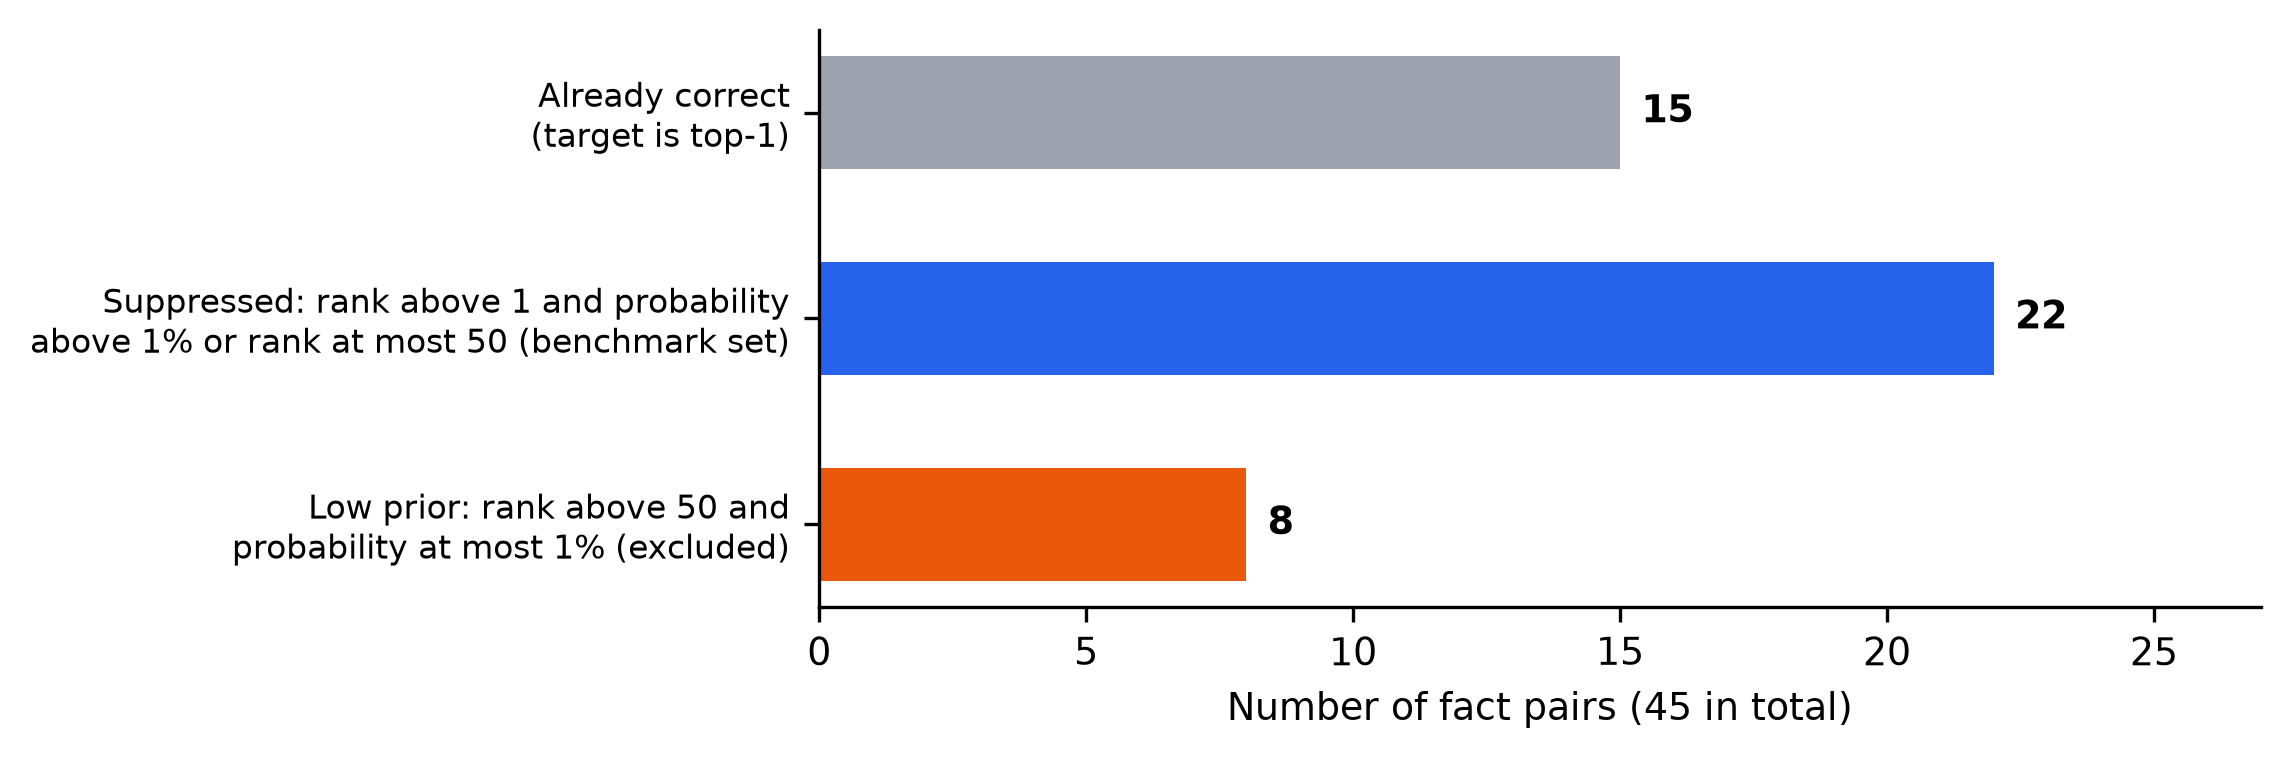
\includegraphics[width=0.8\linewidth]{figures/fig_elig_v2}
\caption{Eligibility Classification of the 45 ROME Fact Pairs}\label{fig:elig}
\end{figure}

The fact bank holds 45 pairs (earlier project notes spoke of 46; re-running the rule on the 45 pairs in the code reproduces 15, 22 and 8). The scan also exposed a separate prompt-format effect: because GPT-2 Small is not instruction-tuned, question-style prompts often continue grammatically rather than factually, so only cloze-style templates are used.

\subsection{The CounterFact Hard Set and Its Split}

The 45 facts are too few and too templated for held-out testing, so a larger benchmark was built from CounterFact (21,919 records, 34 relations; Figure~\ref{fig:pipeline}). Each record gives a prompt (a relation template filled with the subject) and its true answer. A record is kept when the true answer is a single GPT-2 token and the clean model does not rank it first. One batched clean pass per prompt gives the rank; prompts at rank 2 to 1000 are kept, because rank 1 needs no edit and rank above 1000 is too remote for the methods studied. Of 21,913 usable records, 1,817 were already at rank 1 and 3,736 were above rank 1000, leaving \textbf{16,360 prompts} (15,594 distinct subjects). Table~\ref{tab:hardset} gives the counts by starting-rank band.

\begin{table}[H]
\centering
\caption{CounterFact Hard Set by Starting Rank of the True Answer}\label{tab:hardset}
{\small\renewcommand{\arraystretch}{1.15}
\begin{tabular}{|>{\raggedright\arraybackslash}p{0.233\linewidth}|>{\raggedleft\arraybackslash}p{0.204\linewidth}|>{\raggedleft\arraybackslash}p{0.204\linewidth}|>{\raggedleft\arraybackslash}p{0.233\linewidth}|}
\hline
\textbf{Starting rank band} & \textbf{Prompts} & \textbf{Share} & \textbf{Test prompts} \\ \hline
2--5 & 2,765 & 16.9\% & 67 \\ \hline
6--20 & 2,861 & 17.5\% & 76 \\ \hline
21--100 & 4,334 & 26.5\% & 78 \\ \hline
101--1000 & 6,400 & 39.1\% & 79 \\ \hline
All & 16,360 & 100\% & 300 \\ \hline
\end{tabular}}
\end{table}

\begin{figure}[H]
\centering
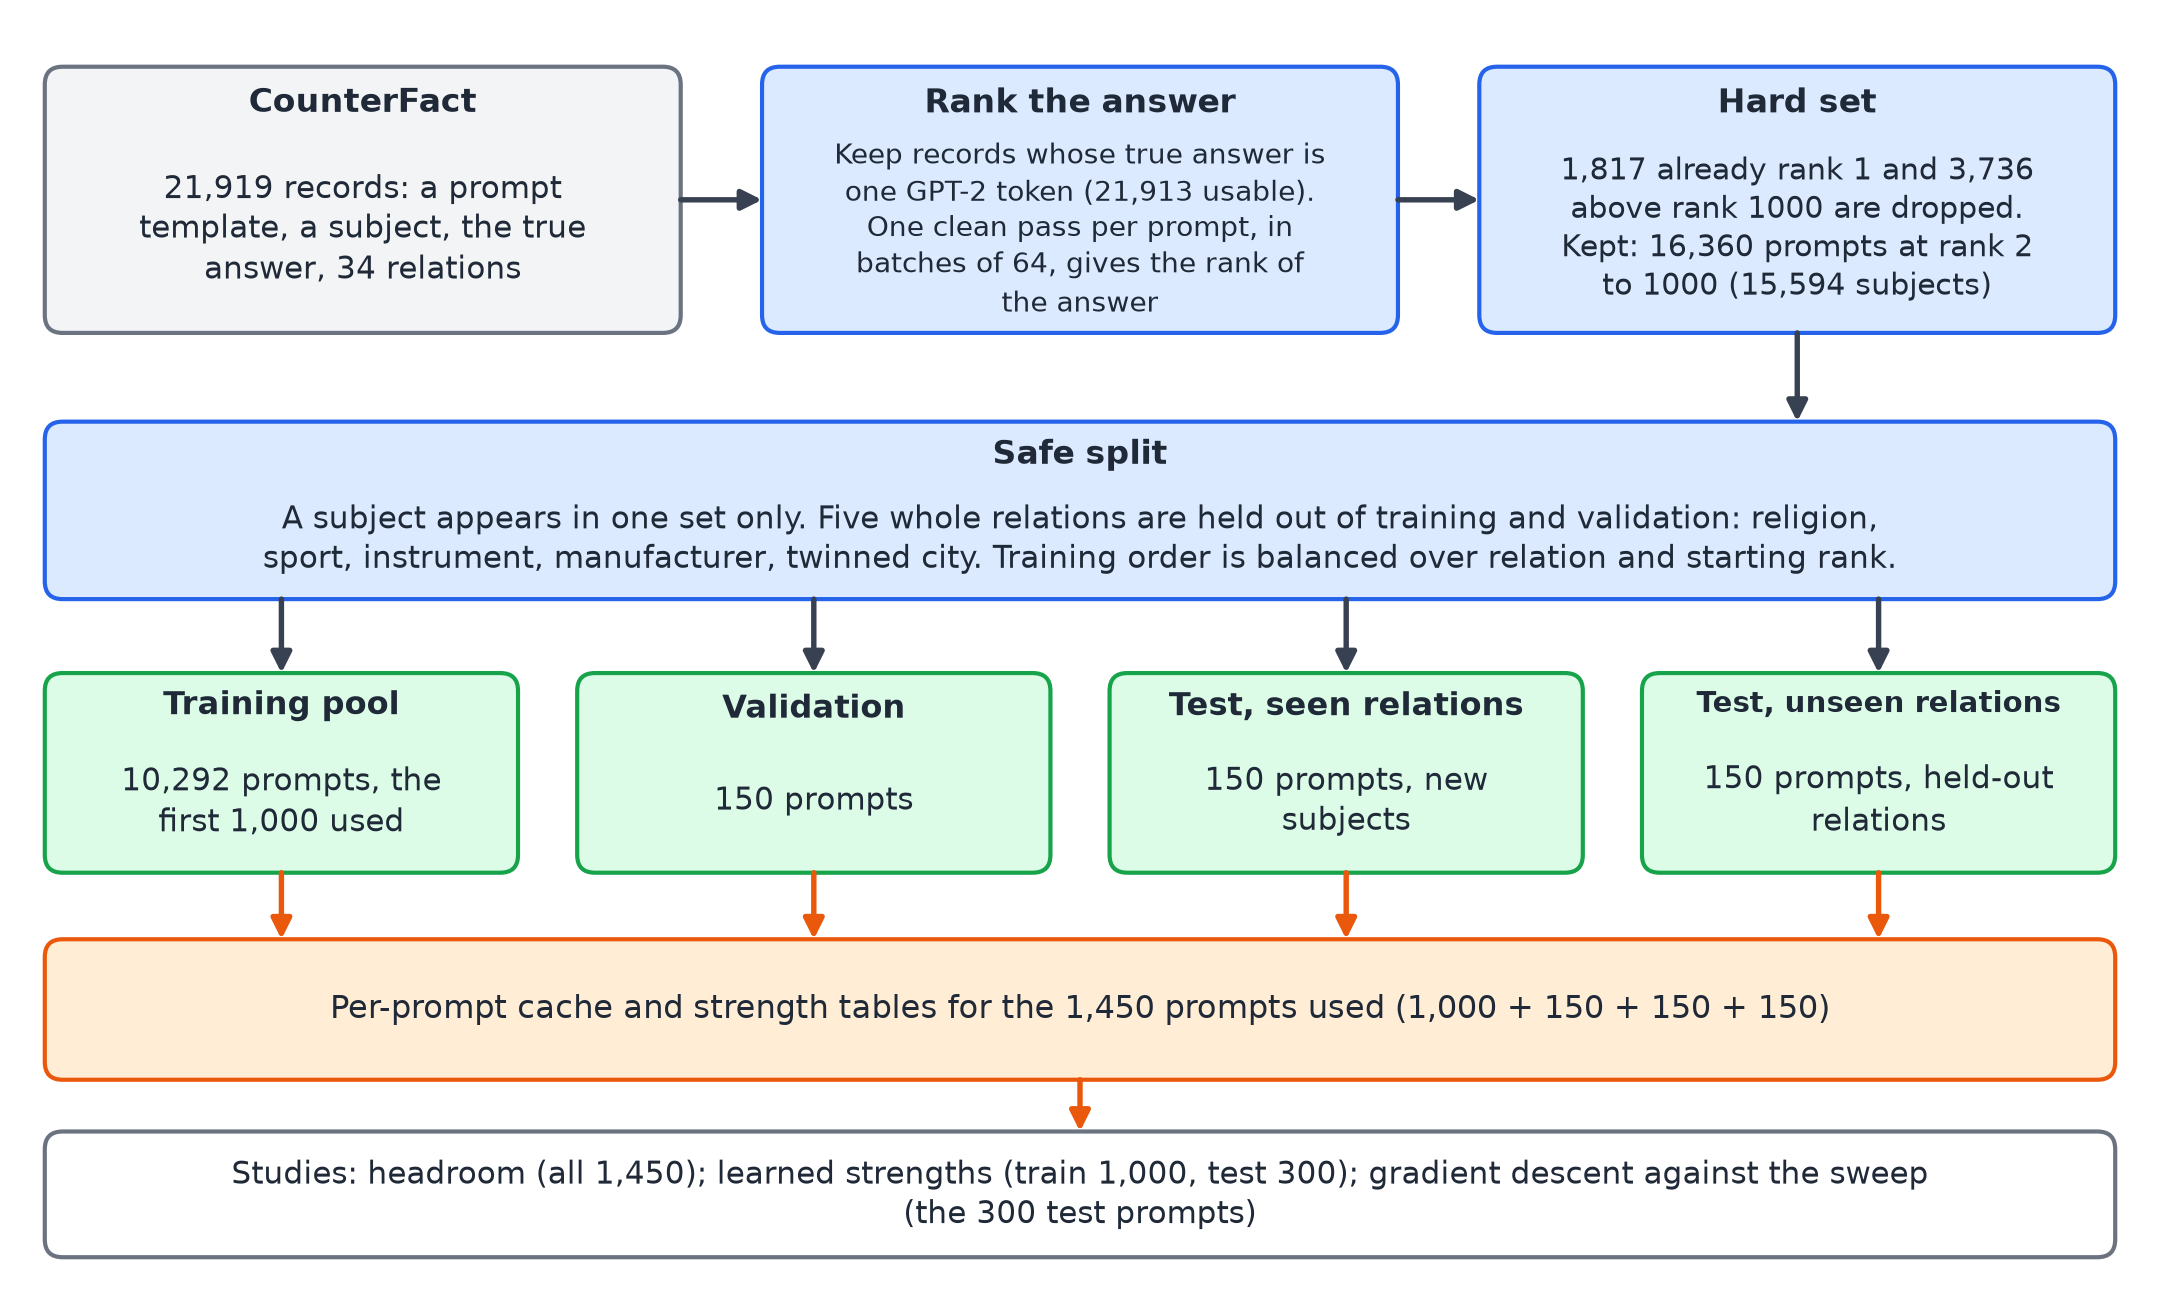
\includegraphics[width=0.95\linewidth]{figures/fig_pipeline}
\caption{Construction of the CounterFact Benchmark: Hard Set, Safe Split, Cache and Strength Tables}\label{fig:pipeline}
\end{figure}

CounterFact reuses 34 templates, so a random split would put near-identical prompts in training and test. The split therefore follows three rules: a subject appears in only one set; five whole relations (religion, sport, instrument, manufacturer, twinned city) are held out of training and validation and form the unseen-relation test; and the training order is balanced over relation and starting-rank band so that its first 250, 500 or 1,000 prompts are each balanced. The sets used are 1,000 training prompts (from a pool of 10,292), 150 validation prompts, 150 test prompts with seen relations and 150 with unseen relations. For these 1,450 prompts a per-prompt cache (the layer-8 state at every position, the candidate features and their activations, and the effect of switching each candidate off) and a set of strength tables (the safety filter's verdict on each candidate at several strengths) were precomputed once, so that later studies never repeat the slow work.

\section{System Architecture}

The system follows a three-tier architecture (Figure~\ref{fig:arch}). The \textbf{presentation tier} is \texttt{experiment\_\allowbreak{}app.\allowbreak{}py}, a Streamlit application with seven tabs (Hybrid mute and boost; Monosemanticity Analysis; Session history and benchmarks; Sequential vs Batched Proof; Batch: Last vs All Tokens; Repair \& SAE limit; Prototype lab), together with command-line entry points (\texttt{run\_\allowbreak{}batch.\allowbreak{}py} and the scripts in \texttt{tools/\allowbreak{}}). The two first applications, \texttt{app.\allowbreak{}py} for single-prompt investigation and \texttt{layer\_\allowbreak{}benchmark.\allowbreak{}py} for multi-layer sweeps, are kept for reference (Appendix~A). The \textbf{intervention engine tier} contains the hooks, the selection and safety logic, the batched evaluation, the Hybrid sweep, the gradient-descent editor, the batch engine and analysis tools, the repair diagnostics and the learned-strength models, and is independent of the user interface. The \textbf{model and data tier} provides cached access to GPT-2 Small, the per-layer SAE dictionaries, the fact datasets, and the per-prompt cache and tables. A device layer selects CUDA, Apple MPS or CPU and provides device-aware synchronisation.

\begin{figure}[H]
\centering
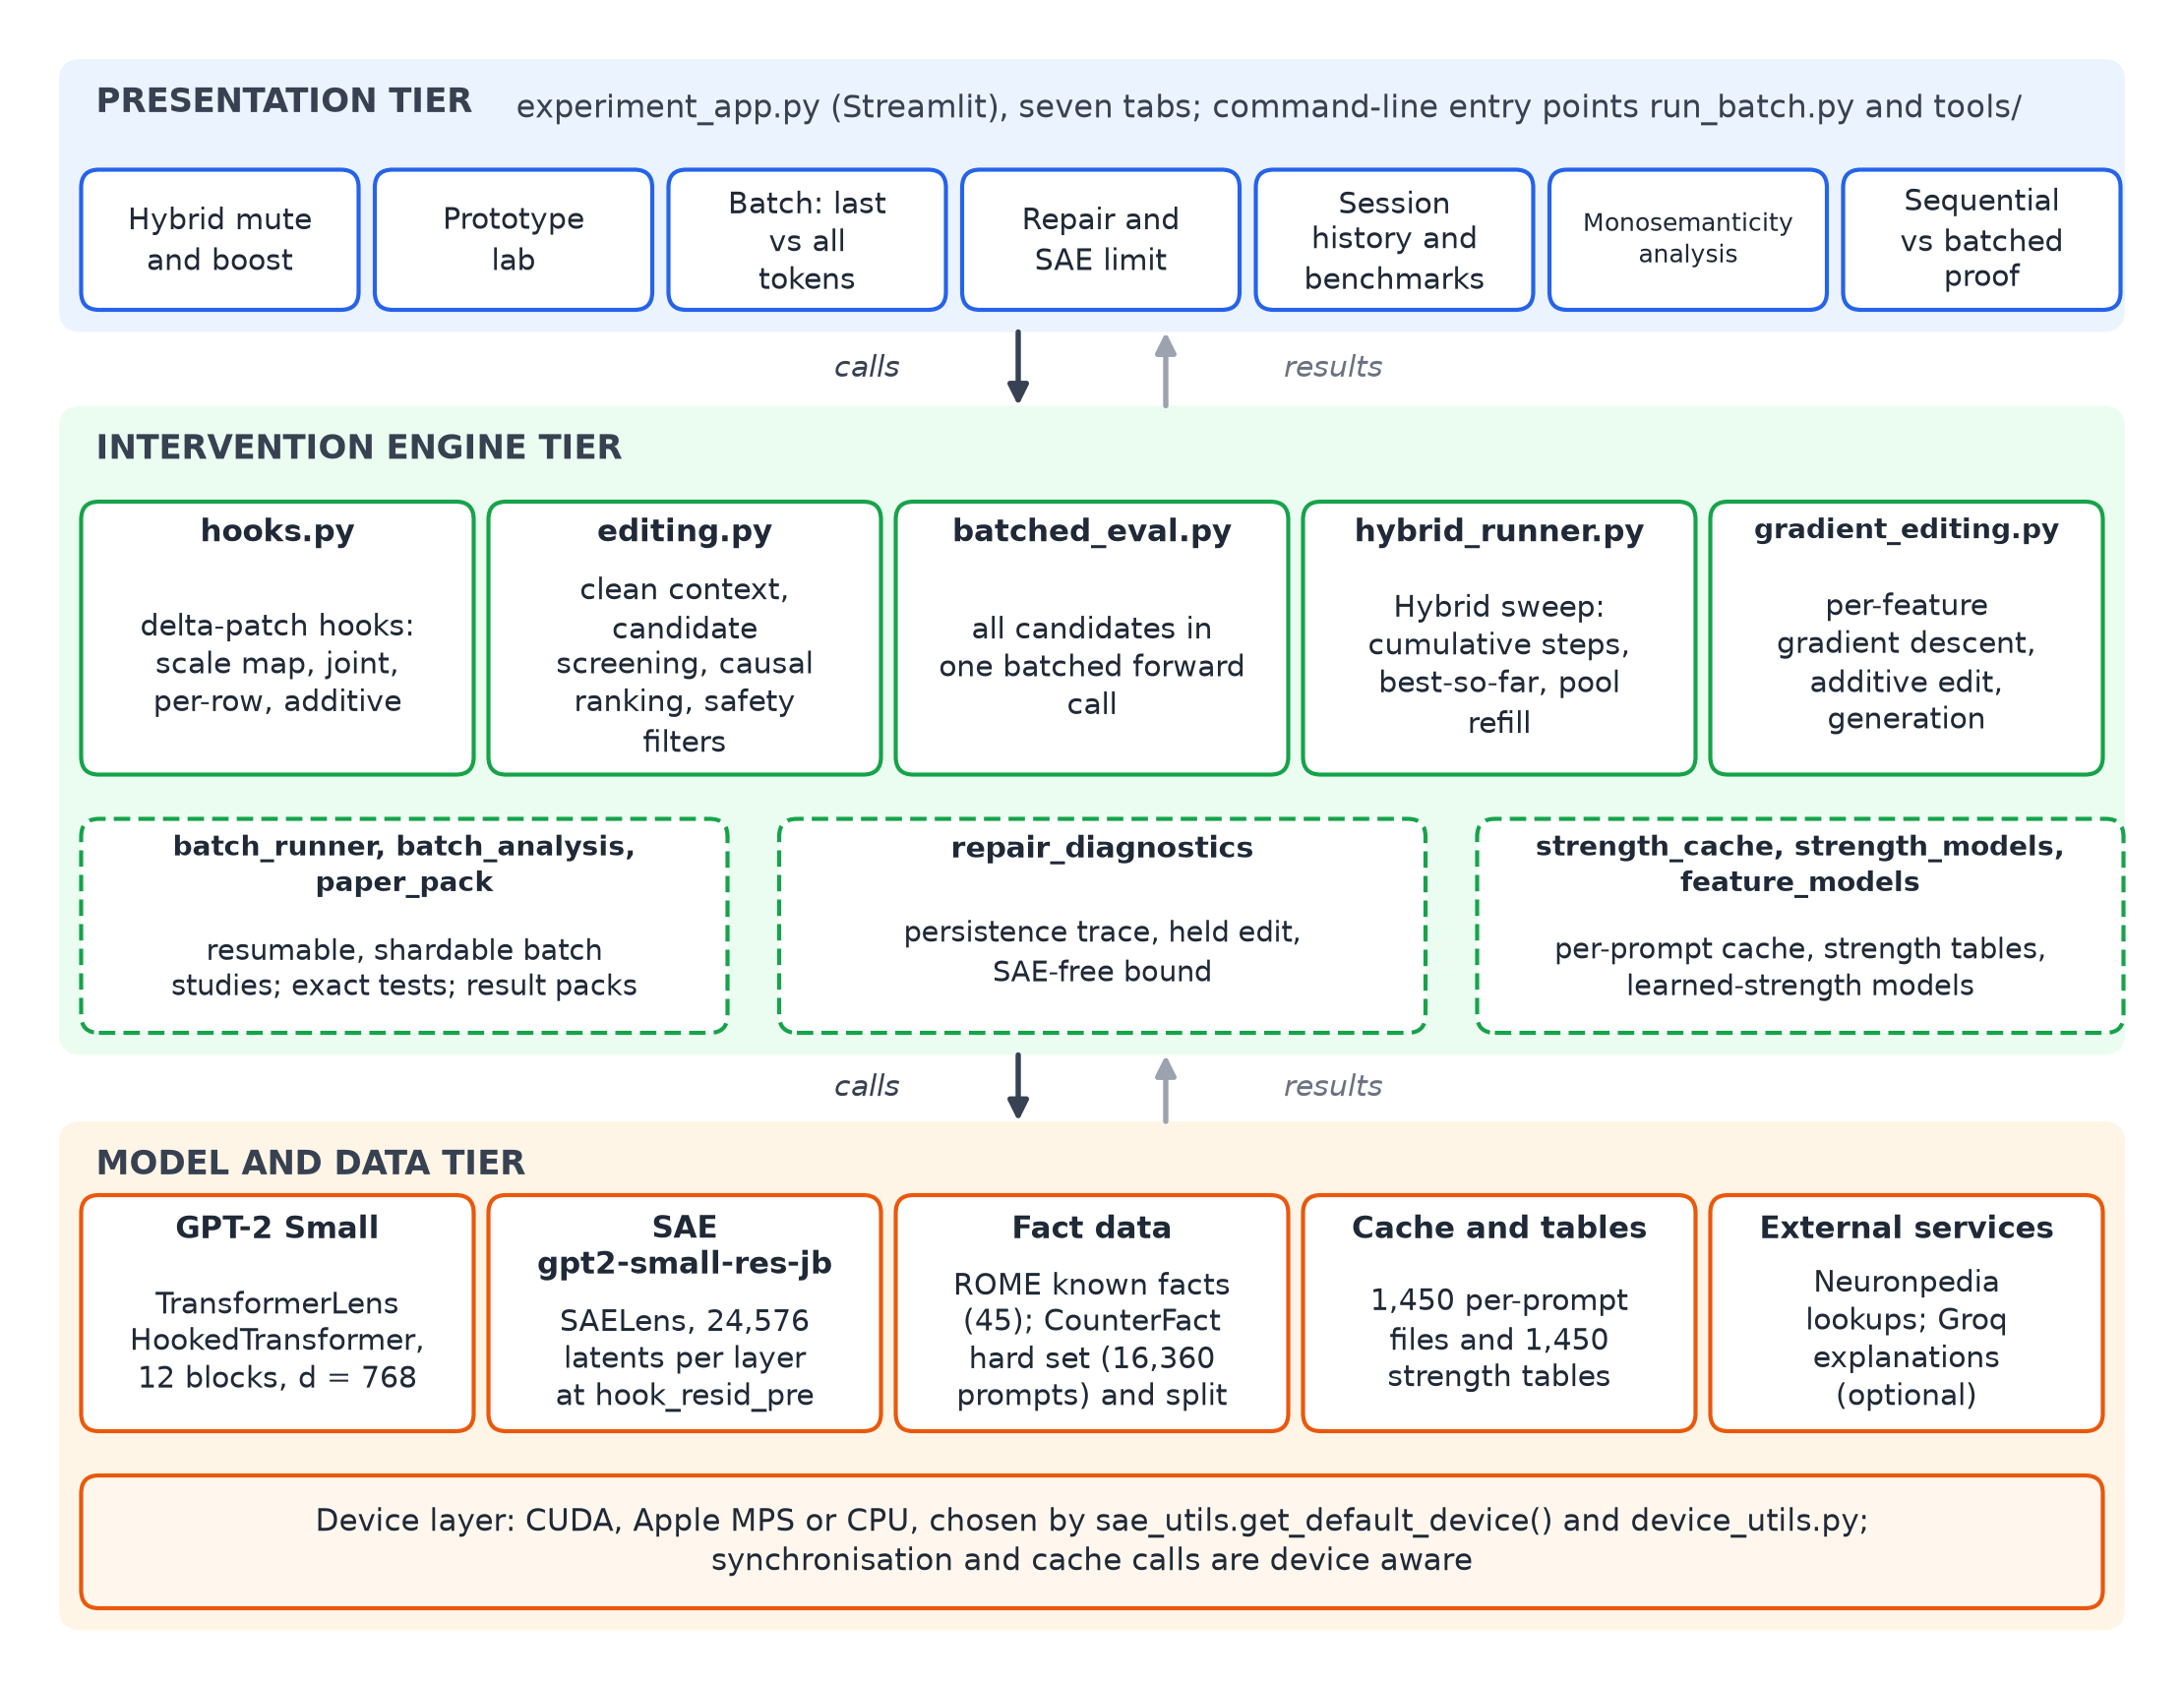
\includegraphics[width=0.98\linewidth]{figures/fig_arch_v2}
\caption{Three-Tier System Architecture}\label{fig:arch}
\end{figure}

The intervention point is the residual stream at \texttt{blocks.\allowbreak{}L.\allowbreak{}hook\_\allowbreak{}resid\_\allowbreak{}pre}. Every attention and MLP block reads from and writes additively into this stream, so an edit there sits downstream of all earlier computation and upstream of all later computation. The SAE is used as a diagnostic instrument that identifies which residual-stream direction corresponds to a concept; the edit itself is applied to the residual stream, not to the SAE or to any weight. The edit acts at every prompt position and, in the generation views, at generated positions as well.

\section{Design Methodology}\label{sec:method}

The design evolved through a hypothesis-driven cycle recorded in a numbered research journal (30 entries by October 2026). Each experiment stated a hypothesis, ran it on a fixed benchmark case (principally the MIT $\rightarrow$ Cambridge prompt), on a small fact set or on held-out prompts, and logged the outcome before the next design change. Optimisation work followed a stricter \textbf{one-bounded-step} rule: identify one bottleneck, measure the reference, implement one change, verify equivalence on a fixed case, log the result, and only then approve the next step. The original sequential code path is retained permanently as the equivalence oracle.

Three practices were added as the project grew. First, every study is stored with its settings, a checksum of the raw result file and per-prompt records, so that a stopped run resumes and a table can be traced to a file. Second, every number is quoted with the set it was measured on, and a stand-in measurement made on cached states is never presented as a result of the real system. Third, results that turned out wrong or misleading were corrected in place and kept on record: the journal documents, among others, a misread success rate, an unfair comparison of edit sizes and a withdrawn inference about knowledge.

\subsection{Sparse Autoencoder Encoding}

For the residual-stream activation $x_p \in \mathbb{R}^{768}$ at token position $p$, the SAE produces feature activations and a reconstruction:

\begin{equation}
f_p = \mathrm{ReLU}\left(W_{\text{enc}}\,(x_p - b_{\text{dec}}) + b_{\text{enc}}\right), \qquad \hat{x}_p = W_{\text{dec}}\, f_p + b_{\text{dec}}
\label{eq:3-1}
\end{equation}

where $f_p \in \mathbb{R}^{24576}$ is sparse (the release subtracts the decoder bias before encoding). Each row $W_{\text{dec}}[i]$ is a direction in residual-stream space associated with feature $i$.

\subsection{Delta Patching}

Replacing $x_p$ with the SAE reconstruction $\hat{x}_p$ would inject the SAE's reconstruction error $e_p = x_p - \hat{x}_p$ and perturb the model even with no intended edit. The system therefore applies only the change in the decoded output, at every position:

\begin{equation}
\Delta_p = \mathrm{Dec}(f'_p) - \mathrm{Dec}(f_p) = \sum_i (s_i - 1)\, f_{p,i}\, W_{\text{dec}}[i], \qquad x'_p = x_p + \Delta_p
\label{eq:3-2}
\end{equation}

where $f'_p$ equals $f_p$ except for the edited latents, which are scaled by $s_i$. Muting with strength $\mu \in [0,1]$ uses $s_i = 1-\mu$ (so $\mu = 1$ is a full ablation); boosting with strength $\beta \ge 0$ uses $s_i = 1+\beta$; the gradient-descent editor uses a free multiplier $s_i = m_i \in [0,3]$. With all $s_i = 1$ the edit is exactly zero. Figure~\ref{fig:delta} shows the operation.

\begin{figure}[H]
\centering
\includegraphics[width=1.0\linewidth]{figures/delta}
\caption{Delta-Patching Intervention at the Residual Stream (the same operation is applied at every prompt position)}\label{fig:delta}
\end{figure}

\subsection{Causal Effect of a Feature}

The causal effect of latent $i$ on token $t$ is the change in the probability of $t$ when $i$ is fully ablated:

\begin{equation}
\Delta p_i(t) = P_{\text{ablate}(i)}(t) - P_{\text{clean}}(t)
\label{eq:3-3}
\end{equation}

Latents are ranked by this quantity rather than by activation magnitude, because the project found empirically that the most strongly activated latent is not necessarily the one that changes the output. Because probabilities pass through a softmax over the whole vocabulary, these deltas are not additive across features. To measure how concentrated a competitor's support is without assuming additivity, the decay ratio relative to the strongest feature is used:

\begin{equation}
D_k = \frac{\left|\Delta p_k\right|}{\left|\Delta p_1\right|}
\label{eq:3-4}
\end{equation}

\subsection{Weighted Competitor Muting (Development Stage)}

In an early version, when several competitors lay above the target, each competitor $c$ received a threat weight proportional to its probability, and the mute strength of its driving features was scaled accordingly and clamped to a ceiling:

\begin{equation}
w_c = \frac{p_c}{\sum_j p_j}, \qquad s_c = \min\left(w_c \cdot s_{\max},\; s_{\max}\right)
\label{eq:3-5}
\end{equation}

This rule was superseded by the sweep below; the code remains in the repository but is not part of the current application.

\subsection{Candidate Selection and the Safety Filter}\label{sec:filter-def}

\textbf{Candidates.} Candidates are features with positive activation. In \textit{last-token} mode they are the features active at the final prompt token; in \textit{all-positions} mode they are the features active at any non-BOS position, each scored by its maximum activation over those positions. A top-$N$ cut by activation is applied first, and $N$ is capped by the number of active features that have not yet been applied. Each candidate is then ablated alone and the change $\Delta p_i$ (Equation~\ref{eq:3-3}) is recorded for the blocking token $c$ (the current top-1 token) and for the target $t$. \textit{Mute candidates} are ordered by $\Delta p_i(c)$, most negative first; \textit{boost candidates} are ordered by $\Delta p_i(t)$ for the target, most negative first, that is, they are the features whose removal hurts the target most.

\textbf{Strict safety filter.} A candidate is tested alone, at the configured strength, against the baseline of the current model state. It is safe if the target's rank does not worsen and its probability does not fall by more than $10^{-6}$ (absolute):

\begin{equation}
\text{safe}(i) \iff r_{\text{edit}(i)}(t) \le r_{\text{base}}(t) \;\wedge\; p_{\text{edit}(i)}(t) - p_{\text{base}}(t) \ge -10^{-6}
\label{eq:3-6}
\end{equation}

The same rule is applied to mute and to boost candidates. A feature that is safe on both sides is kept on one side only, chosen by which side raises the target probability more (or, with the filter off, by its rank in each list), because applying both would multiply the scales by $(1-\mu)(1+\beta) \approx 1$ and waste a feature slot. A separate \textit{combination check} applies a whole set of edits together and reports \textit{new blockers}: tokens that were ranked below the target in the clean model and rise above it. Two relaxed variants of Equation~\ref{eq:3-6} exist only in the batch harness: a \textit{tolerance} variant that also accepts a probability drop of up to 5\% of the current target probability, and a \textit{graded} variant that retries a failing candidate at a fraction of its strength.

\subsection{Cumulative Sweep, Best-So-Far Tracking and Pool Refill}\label{sec:sweep-def}

The safe mute and boost pools, ordered as above, are applied cumulatively. Step $k$ applies the first $\min(k, M)$ mutes and the first $\min(k, B)$ boosts in one forward pass, where $M$ and $B$ are the pool sizes, and the sweep stops as soon as the target reaches rank 1. Combinations of individually safe features are not guaranteed to improve monotonically (Section~\ref{sec:dev-results}), so the lowest target rank seen, with ties broken by higher probability, is tracked, and the best step, not the last, is reported. In \textbf{pool refill}, when a pool is exhausted and the target is not yet rank 1, every applied feature is kept, one forward pass with them applied gives a new baseline, the blocker becomes the top-1 token of the edited model, and the remaining active features are re-ranked and re-filtered against that state, including ones rejected earlier. A run ends at rank 1, when no unapplied active feature remains, when a round yields no safe candidate, or at an optional step limit. The number of features active at the hook position is therefore a hard ceiling on any multiplicative edit at one layer: scaling cannot activate a feature that is off.

\subsection{The Gradient-Descent Editor}\label{sec:gd-def}

The sweep decides which features and how many, with one strength for each side. The gradient-descent editor instead gives every candidate feature its own multiplier and tunes all of them together for the given prompt. The $K$ candidates are the top $N$ features by maximum activation over the prompt positions (BOS excluded). Candidate $k$ has a free number $z_k$ and a multiplier $m_k = 1 + a_k$ with

\begin{equation}
a_k = -1 + 3\,\sigma(z_k), \qquad m_k \in (0, 3)
\label{eq:3-7}
\end{equation}

where $\sigma$ is the logistic function, and all $z_k$ start at the value that gives $a_k = 0$ (no edit). With $A_{p,k}$ the clean activation of candidate $k$ at position $p$, the edit is Equation~\ref{eq:3-2} with $s_k = m_k$:

\begin{equation}
\Delta_p = \sum_{k=1}^{K} a_k\, A_{p,k}\, W_{\text{dec}}[k]
\label{eq:3-8}
\end{equation}

Blocks 8 to 11 are run from the edited state and the logits at the last position are read. The loss for one prompt, with $t$ the target, $b$ the clean top-1 token (the blocker) and $\ell$ the logits of the edited model, is

\begin{equation}
\mathcal{L} = \max\!\left(0,\; \gamma - (\ell_t - \max_{v \ne t} \ell_v)\right) \;+\; \lambda_{\text{KL}}\, \left[\ell_t - \max_{v \ne t}\ell_v \ge \gamma\right]\; \mathrm{KL} \;+\; \lambda_{\text{size}} \sum_k |a_k|\, w_k
\label{eq:3-9}
\end{equation}

with margin $\gamma = 0.3$, $\lambda_{\text{KL}} = 3.0$, $\lambda_{\text{size}} = 0.005$ and $w_k = \max_p A_{p,k} / \sum_j \max_p A_{p,j}$. The bracket is 1 when the condition inside holds and 0 otherwise. The KL term is the divergence $\mathrm{KL}(p_{\text{clean}} \,\Vert\, p_{\text{edited}})$ at the last position over all tokens except $t$ and $b$, renormalised, so that the intended change is not penalised (Equation~\ref{eq:3-10}). It is charged only once the target leads, which mirrors the sweep's stopping rule, but means that a failing edit is not discouraged from distorting the output; an option charges it on every step.

\begin{equation}
\mathrm{KL} = \sum_{v \notin \{t,b\}} q_v \log\frac{q_v}{\tilde{p}_v}, \qquad q = \mathrm{softmax}(\ell^{\text{clean}}_{\setminus\{t,b\}}), \quad \tilde{p} = \mathrm{softmax}(\ell_{\setminus\{t,b\}})
\label{eq:3-10}
\end{equation}

The free numbers are updated by the Adam optimiser \cite{r36} with learning rate 0.1 for 100 steps, with gradients taken with respect to $z$ only, so that no model weight is changed or even given a gradient. The iterate kept is the one with the lowest loss among those where the target is rank 1, or, if none reaches rank 1, the one with the lowest loss. The chosen multipliers are finally applied through the same delta-patch hook that the sweep uses, in a full forward pass, and the reported rank, probability, top-1 token and KL come from that pass; the tuning-pass rank is compared with it and any difference is flagged. Table~\ref{tab:gdsettings} lists the settings.

\begin{table}[H]
\centering
\caption{Settings of the Gradient-Descent Editor (Defaults)}\label{tab:gdsettings}
{\small\renewcommand{\arraystretch}{1.15}
\begin{tabular}{|>{\raggedright\arraybackslash}p{0.283\linewidth}|>{\raggedright\arraybackslash}p{0.141\linewidth}|>{\raggedright\arraybackslash}p{0.476\linewidth}|}
\hline
\textbf{Setting} & \textbf{Default} & \textbf{Role} \\ \hline
Candidate features $N$ & 200 & How many features may be edited (the application default is 30; the studies use 200) \\ \hline
Candidate source & All prompt positions & Alternative: last token only \\ \hline
Steps & 100 & Number of gradient updates \\ \hline
Learning rate & 0.1 & Size of each update of $z$ \\ \hline
Rank-1 margin $\gamma$ & 0.3 & Required lead over the strongest competing token, in logits \\ \hline
Side-effect weight $\lambda_{\text{KL}}$ & 3.0 & Strength of the KL penalty, charged once the target leads \\ \hline
Edit-size weight $\lambda_{\text{size}}$ & 0.005 & Penalty on large multiplier changes, weighted by feature activity \\ \hline
Multiplier range & 0 to 3 & From the feature removed to the feature tripled; 1 leaves it alone \\ \hline
\end{tabular}}
\end{table}

\subsection{Additive Extension (Exploratory)}\label{sec:additive-def}

A multiplier cannot switch on a feature that is silent, since $0 \times m = 0$. An optional additive term therefore adds an amount $c_k \ge 0$ of the decoder direction of selected silent features at the last position only. The candidates are the 200 silent features with the highest first-order score, that is, the dot product of the feature's decoder direction with the gradient of the target margin with respect to the residual; each amount starts at exactly zero, is capped at a multiple of the loudest feature active on the prompt, and carries an extra loss $0.005 \sum_k c_k / \text{cap}$. This extension is off by default in the application and is reported in Section~\ref{sec:additive} mainly as a negative result.

\section{Flow Diagrams}

\subsection{Data Flow Diagram: Level 0 (Context Diagram)}

The Level 0 DFD (Figure~\ref{fig:dfd0}) represents the system as a single process interacting with four external entities: the \textbf{Researcher}, who supplies prompts, targets and intervention parameters and receives ranks, probabilities and artifacts; the \textbf{Fact Dataset}; the \textbf{GPT-2 Small} model, which executes hooked forward passes; and the \textbf{Pretrained SAEs}, which encode and decode residual activations.

\begin{figure}[H]
\centering
\includegraphics[width=0.92\linewidth]{figures/dfd0}
\caption{DFD Level 0: Context Diagram}\label{fig:dfd0}
\end{figure}

\subsection{Data Flow Diagram: Level 1}

The Level 1 DFD (Figure~\ref{fig:dfd1}) decomposes the Hybrid sweep into eight processes and one data store. Process 1.0 (\textit{Eligibility Classification}) admits only prompts whose target is not already top-1. Process 2.0 (\textit{Clean Baseline}) records the target's rank, probability and the competitors above it. Process 3.0 (\textit{Sparse Screening}) encodes the residual stream and returns the top-$N$ active latents. Process 4.0 (\textit{Causal Ranking}) ranks these by their effect on competitors and on the target. Process 5.0 (\textit{Safety Filtering}) removes unsafe candidates. Process 6.0 (\textit{Joint Intervention}) applies the combined edit. Processes 7.0 and 8.0 compute metrics, persist JSON artifacts to data store D1 and render results. The figure was drawn for the original last-token pipeline; the refill loop is shown in Figure~\ref{fig:algo}, and the gradient-descent path, which replaces processes 4.0 to 6.0 by one optimisation, in Figure~\ref{fig:gdflow}.

\begin{figure}[H]
\centering
\includegraphics[width=0.95\linewidth]{figures/dfd1}
\caption{DFD Level 1: Expanded Intervention Pipeline (original version)}\label{fig:dfd1}
\end{figure}

\subsection{Hybrid Mute \& Boost Control Flow}

Figure~\ref{fig:algo} shows the control flow of the sweep for a single prompt at a single layer, including the cumulative steps, the best-step rule and the pool-refill loop.

\begin{figure}[H]
\centering
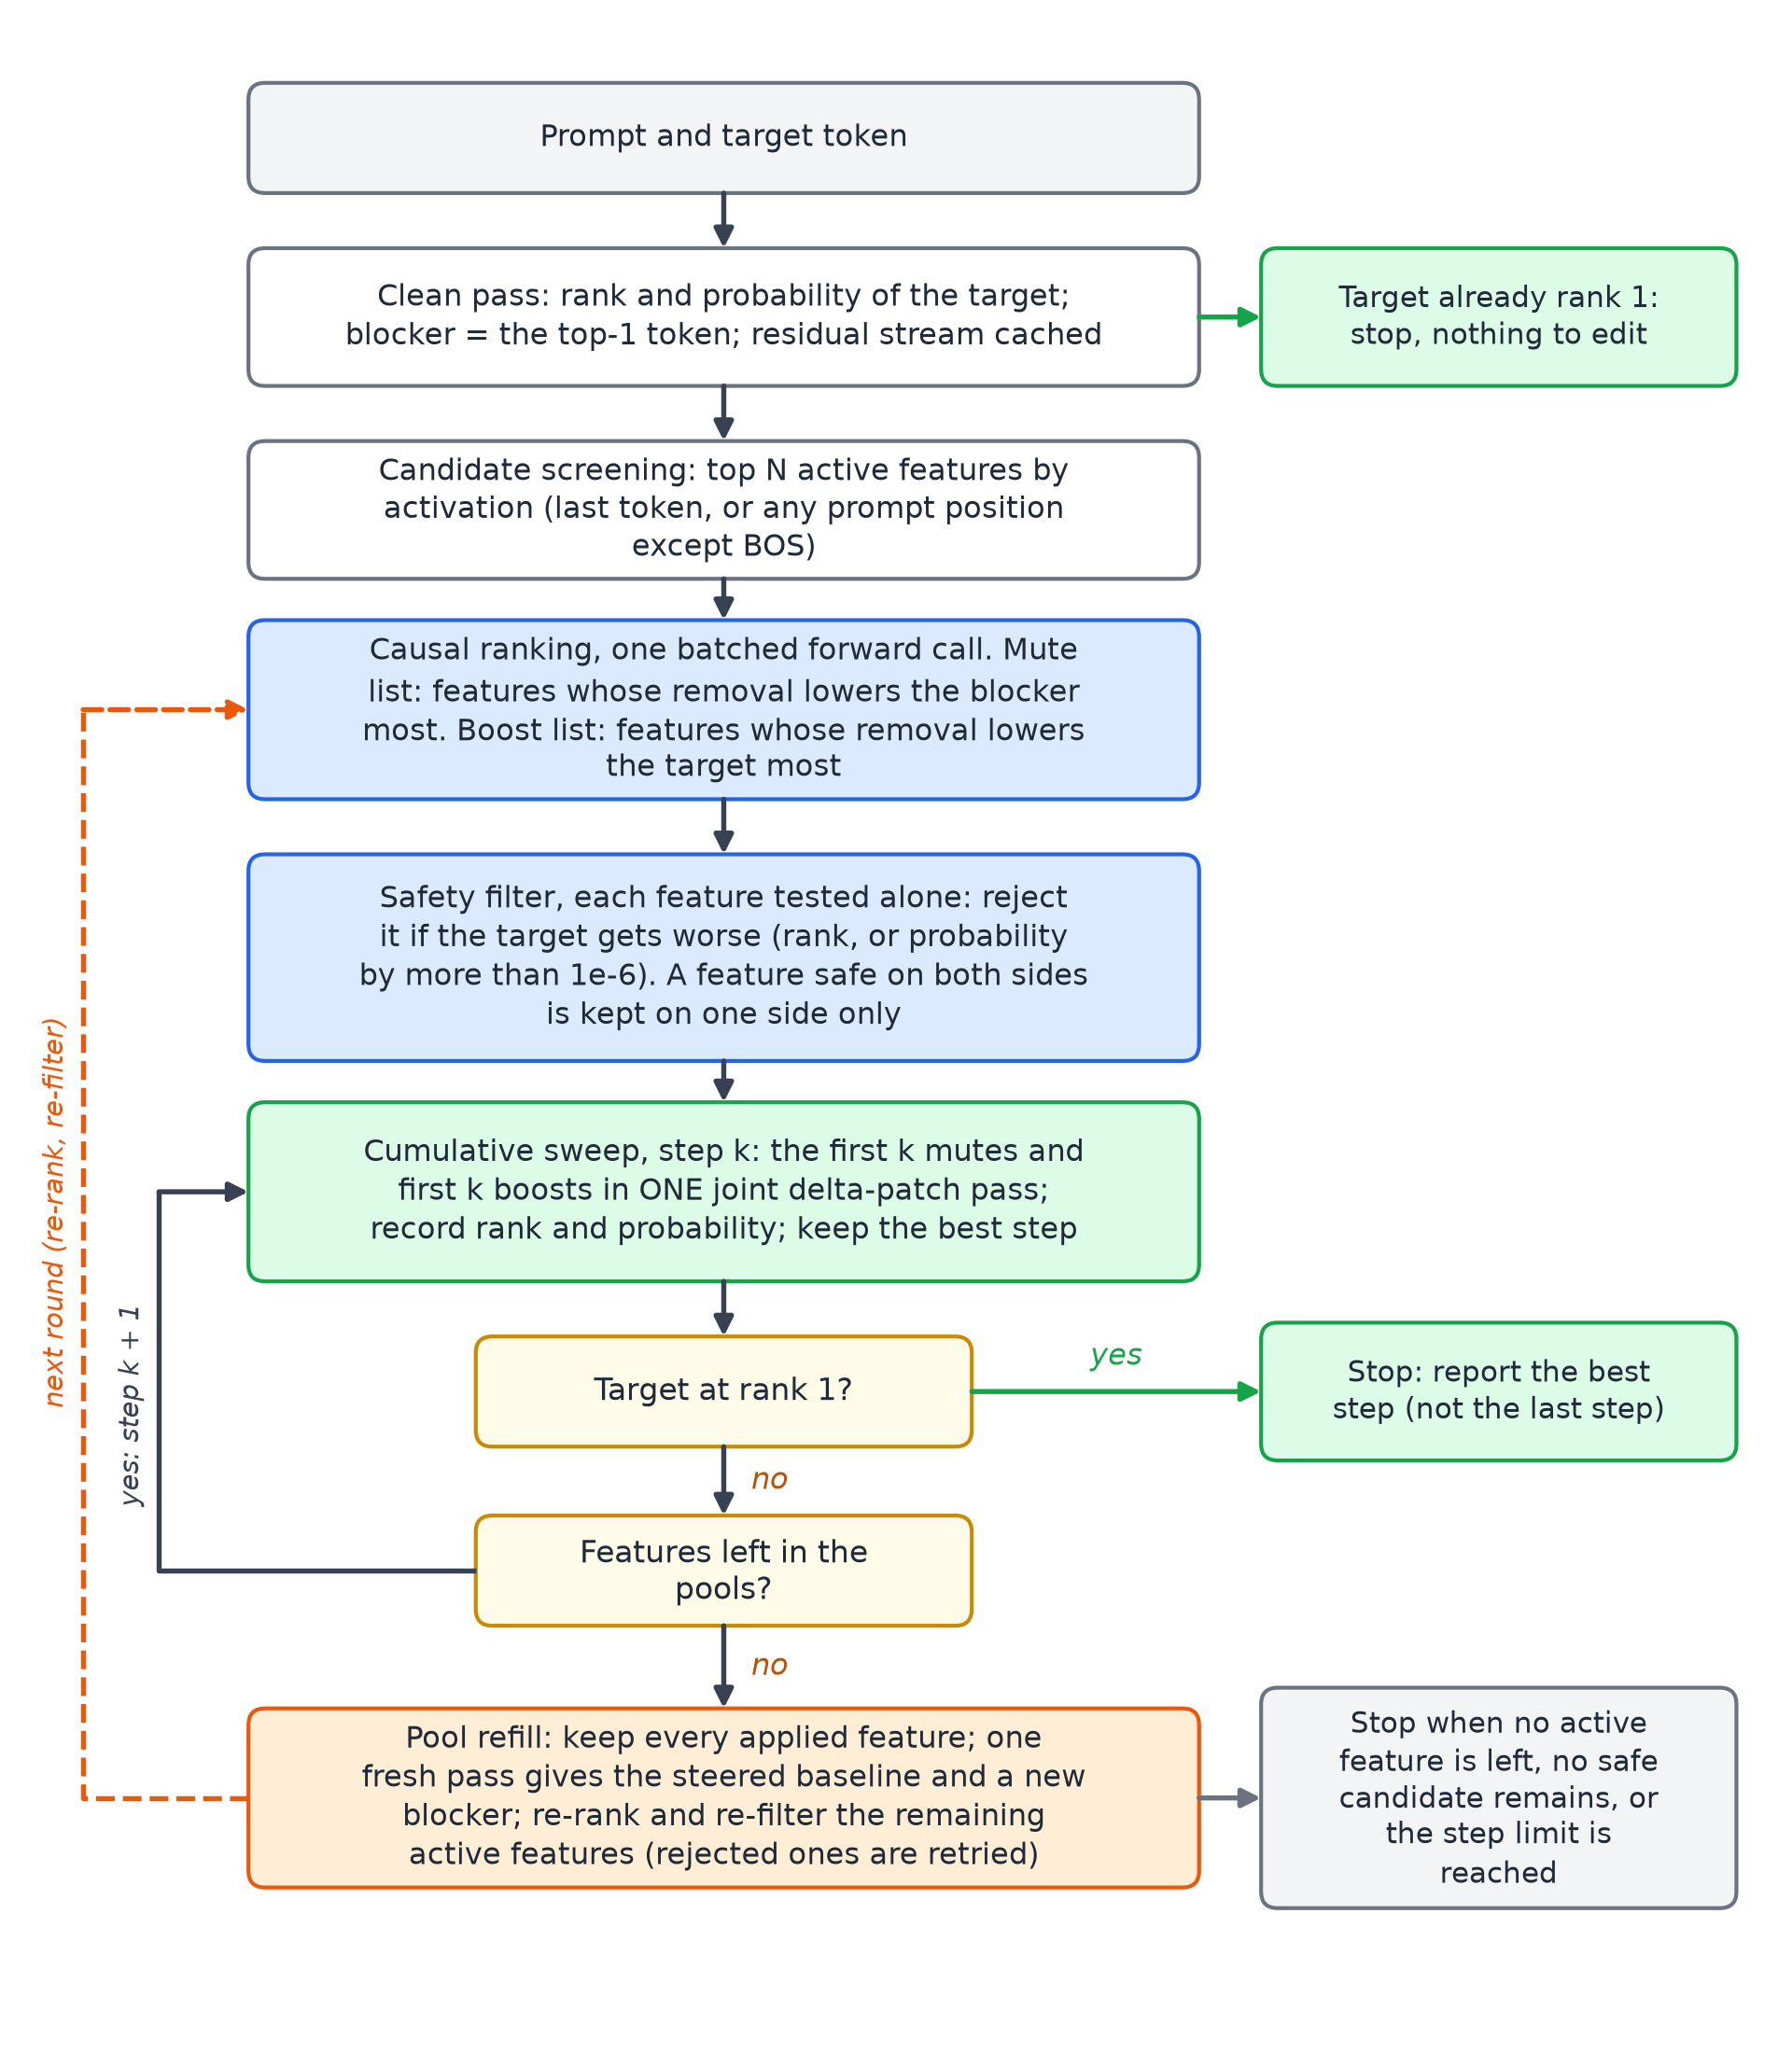
\includegraphics[width=0.72\linewidth]{figures/fig_algo_v2}
\caption{Control Flow of the Hybrid Mute \& Boost Sweep with Pool Refill}\label{fig:algo}
\end{figure}

\subsection{Gradient-Descent Editor Flow}

Figure~\ref{fig:gdflow} shows the gradient-descent editor: the free numbers, the edit at every position, the run through blocks 8 to 11, the loss and the update, and the final check through the real hook.

\begin{figure}[H]
\centering
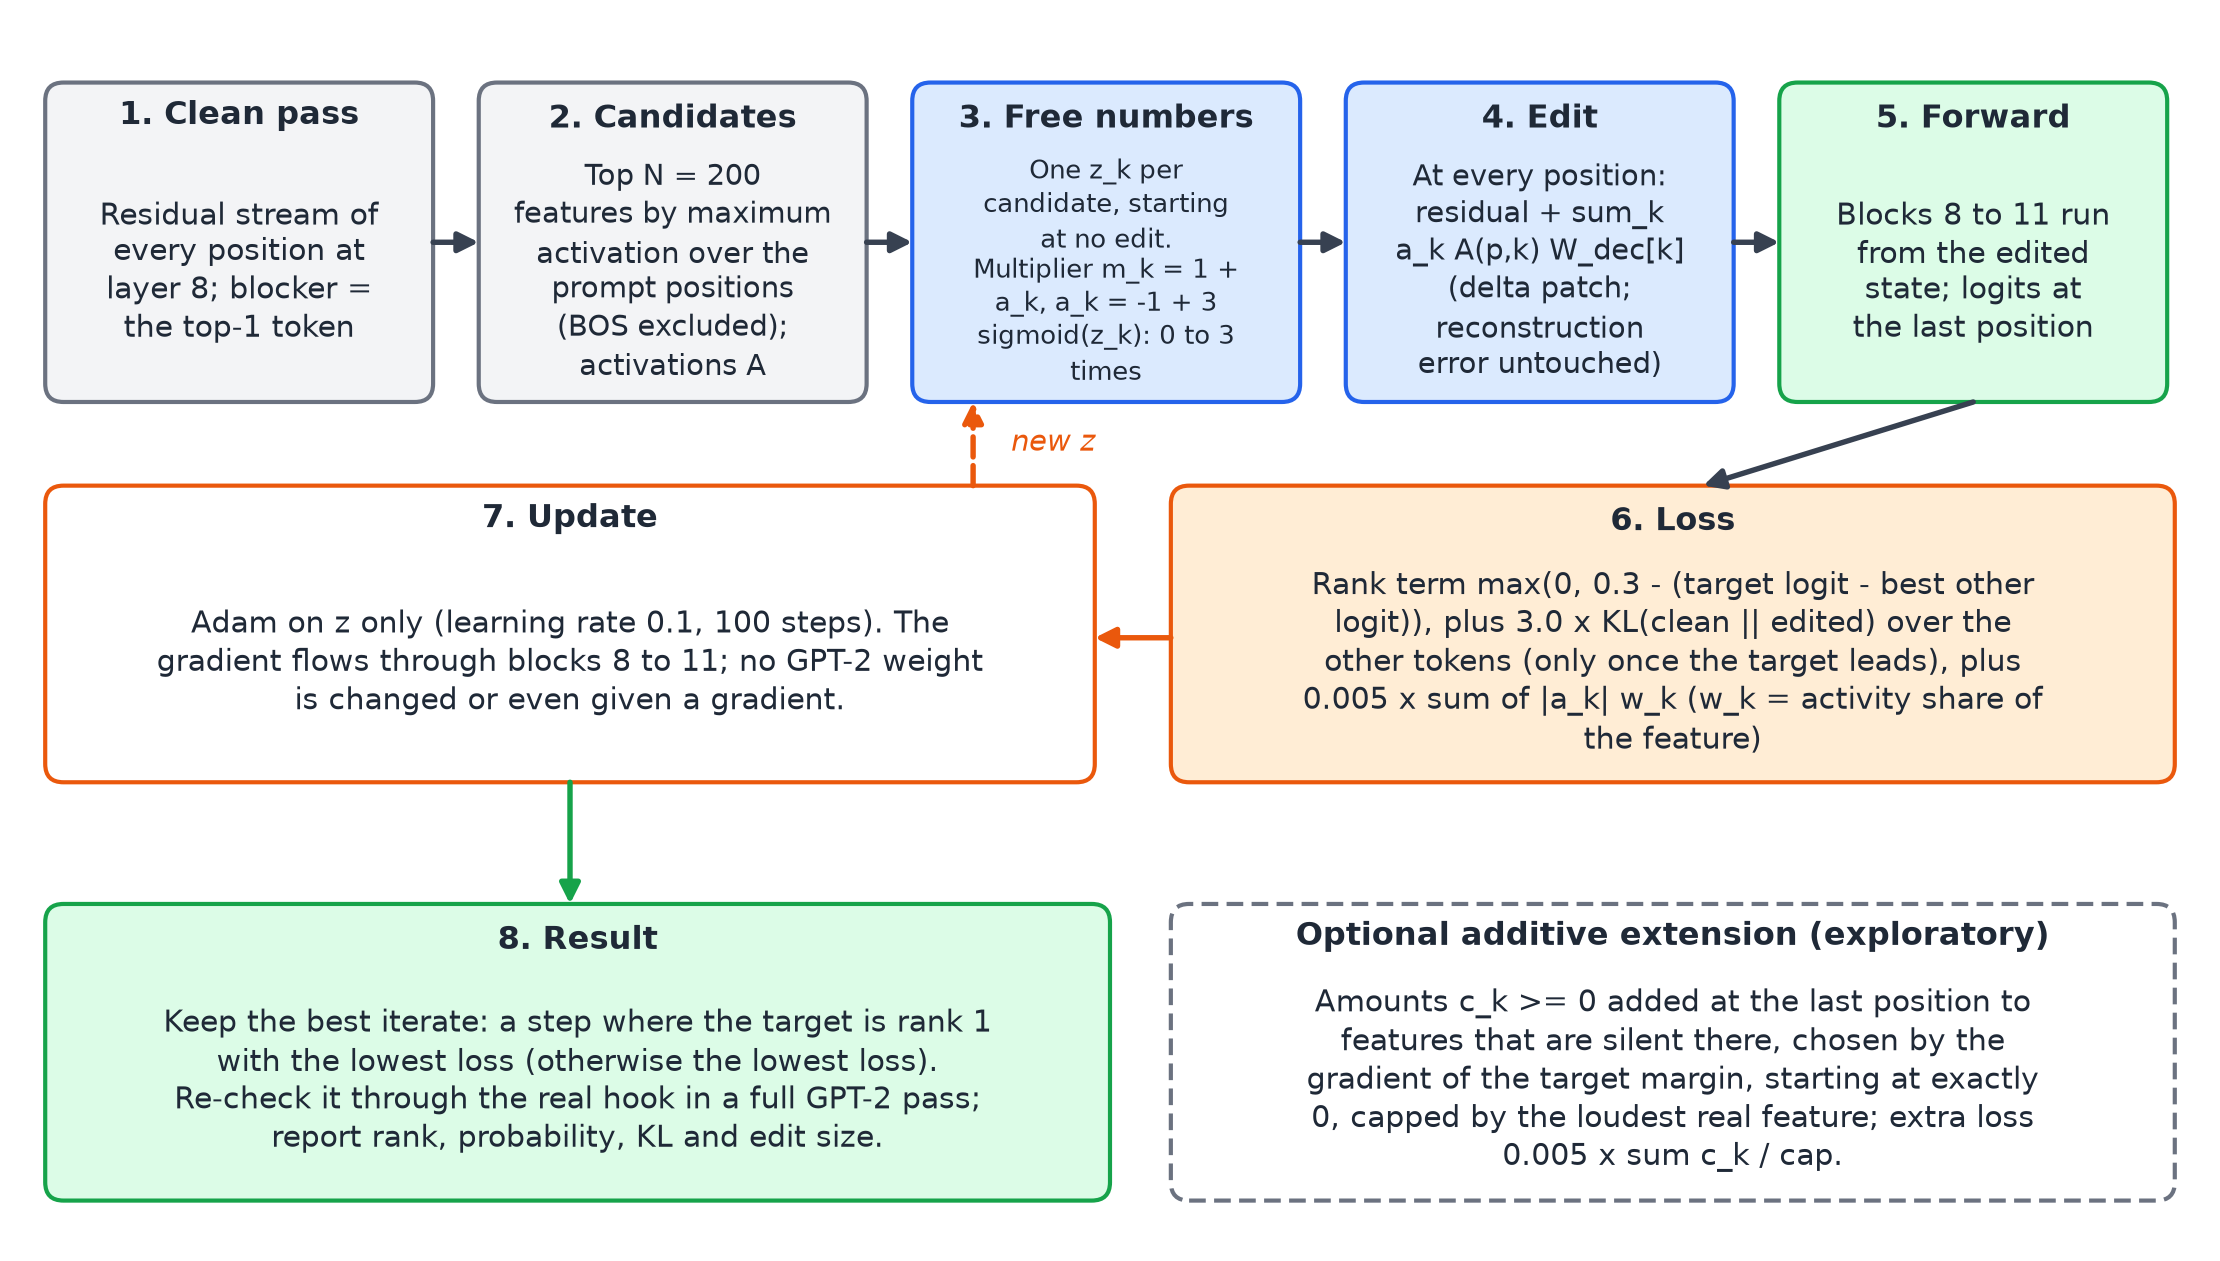
\includegraphics[width=0.98\linewidth]{figures/fig_gd_flow}
\caption{Flow of the Gradient-Descent Editor}\label{fig:gdflow}
\end{figure}

\section{Modules of the Project}

The system is divided into the following functional modules:

\begin{enumerate}
  \item \textbf{Model and SAE Loading (\texttt{src/\allowbreak{}sae\_\allowbreak{}utils.\allowbreak{}py}, \texttt{src/\allowbreak{}device\_\allowbreak{}utils.\allowbreak{}py}):} detects the compute device (CUDA, Apple MPS or CPU; an environment variable can force one), loads GPT-2 Small as a TransformerLens \texttt{HookedTransformer} and the layer-specific SAEs from SAELens. The $\sim$500 MB base model is instantiated once per session while each SAE is cached independently; the device helpers synchronise and free memory correctly on each backend.
  \item \textbf{Hooking (\texttt{src/\allowbreak{}hooks.\allowbreak{}py}):} forward hooks that encode the residual stream, scale selected latents, decode and add only the delta (Equation~\ref{eq:3-2}): single, joint, combined mute-and-boost, scale-map, per-row batched and additive hooks.
  \item \textbf{Causal Selection (\texttt{src/\allowbreak{}editing.\allowbreak{}py}):} clean and steered contexts, candidate screening (last token or all positions), causal ranking for the target and the competitor, the single, batched and combination safety checks, and the development-stage weighted reduction.
  \item \textbf{Batched Evaluation (\texttt{src/\allowbreak{}batched\_\allowbreak{}eval.\allowbreak{}py}):} evaluates many candidates as one batched forward call.
  \item \textbf{Evaluation (\texttt{src/\allowbreak{}evaluation.\allowbreak{}py}, \texttt{src/\allowbreak{}fact\_\allowbreak{}bank.\allowbreak{}py}):} the eligibility rule, the ROME-sourced fact bank and the specificity check against unrelated control prompts.
  \item \textbf{Hybrid Sweep (\texttt{src/\allowbreak{}hybrid\_\allowbreak{}runner.\allowbreak{}py}):} the headless port of the Hybrid tab, with the cumulative sweep, best-so-far tracking, pool refill, safety modes and side-effect measurement.
  \item \textbf{Gradient-Descent Editor (\texttt{src/\allowbreak{}gradient\_\allowbreak{}editing.\allowbreak{}py}):} the optimiser of Section~\ref{sec:gd-def}, the additive extension, greedy generation with the edit on or off, and the next-word shift on follow-up prompts.
  \item \textbf{Batch Engine and Result Packs (\texttt{src/\allowbreak{}batch\_\allowbreak{}runner.\allowbreak{}py}, \texttt{src/\allowbreak{}batch\_\allowbreak{}analysis.\allowbreak{}py}, \texttt{src/\allowbreak{}paper\_\allowbreak{}pack.\allowbreak{}py}, \texttt{run\_\allowbreak{}batch.\allowbreak{}py}):} resumable, shardable runs of many prompts under several arms, exact paired tests, and labelled tables, figures and provenance.
  \item \textbf{Layer Benchmark (\texttt{src/\allowbreak{}benchmark/\allowbreak{}layer\_\allowbreak{}benchmark\_\allowbreak{}runner.\allowbreak{}py}):} the UI-independent layer sweep with stage profiling, forward-pass accounting and JSON artifacts.
  \item \textbf{Diagnostics and Learned-Strength Models (\texttt{src/\allowbreak{}repair\_\allowbreak{}diagnostics.\allowbreak{}py}, \texttt{src/\allowbreak{}strength\_\allowbreak{}cache.\allowbreak{}py}, \texttt{src/\allowbreak{}strength\_\allowbreak{}models.\allowbreak{}py}, \texttt{src/\allowbreak{}feature\_\allowbreak{}models.\allowbreak{}py}):} persistence tracing and the SAE-free bound, the per-prompt cache and strength tables, and the strength predictors.
  \item \textbf{Studies and Checks (\texttt{tools/\allowbreak{}}):} scripts that build the benchmark, run and summarise each study, draw the journal and report figures, and check equivalence (Section~\ref{sec:checks}).
  \item \textbf{Presentation (\texttt{experiment\_\allowbreak{}app.\allowbreak{}py}; early versions \texttt{app.\allowbreak{}py}, \texttt{layer\_\allowbreak{}benchmark.\allowbreak{}py}):} the Streamlit interfaces (Appendix~A).
\end{enumerate}

\section{Operating Environment}

\begin{table}[H]
\centering
\caption{Software and Hardware Requirements}\label{tab:environment}
{\small\renewcommand{\arraystretch}{1.15}
\begin{tabular}{|>{\raggedright\arraybackslash}p{0.285\linewidth}|>{\raggedright\arraybackslash}p{0.643\linewidth}|}
\hline
\textbf{Component} & \textbf{Specification} \\ \hline
Operating system & Windows 11 (development and all timed studies); macOS on Apple silicon (port); Linux compatible \\ \hline
Language & Python 3.13 (Windows), Python 3.12 (macOS) \\ \hline
Deep learning framework & PyTorch 2.6.0 with CUDA 12.4 (GTX 1660 Ti PC); 2.5.1 with CUDA 12.1 (RTX 4050 laptop); 2.13.0 with MPS (macOS) \\ \hline
Interpretability libraries & TransformerLens 3.5.1, SAELens 6.45.3 \\ \hline
Language model & GPT-2 Small (124M parameters, 12 blocks, $d_{\text{model}}$ = 768) \\ \hline
SAE release & gpt2-small-res-jb (24,576 latents per layer, hook\_resid\_pre) \\ \hline
Feature lookup & Neuronpedia \\ \hline
User interface & Streamlit 1.59.1 \\ \hline
Model hosting & Hugging Face Hub (authenticated via HF\_TOKEN) \\ \hline
Version control & Git; the work reported here is on the branch gradient-descent-editing \\ \hline
GPUs & NVIDIA GeForce GTX 1660 Ti (6 GB); NVIDIA RTX 4050 Laptop GPU (6 GB); Apple silicon GPU through MPS \\ \hline
Peak memory & about 1.45 GB of GPU memory for a four-layer benchmark \\ \hline
\end{tabular}}
\end{table}

% ------------------------------------------------------------
\chapter{Implementation}\label{ch:implementation}

\section{Technologies Used}

\textbf{PyTorch} \cite{r22} provides tensor computation, automatic differentiation and GPU acceleration on CUDA and on Apple's MPS backend. \textbf{TransformerLens} \cite{r13} exposes GPT-2 Small as a \texttt{HookedTransformer} in which every intermediate activation has a named hook point, so functions can read or replace activations during a forward pass and the model can be run from a saved intermediate state. \textbf{SAELens} \cite{r14} loads the pretrained \texttt{gpt2-small-res-jb} dictionaries \cite{r15} and provides \texttt{encode} and \texttt{decode} operations. \textbf{Neuronpedia} \cite{r20} was used to inspect what individual features respond to. \textbf{Streamlit} provides the browser-based application, with \texttt{@st.\allowbreak{}cache\_\allowbreak{}resource} used for model and SAE caching. Optional natural-language explanations of a run are requested from the Groq inference service. The gradient-descent editor uses the Adam optimiser \cite{r36}. Results are stored as JSON and JSON lines, and the report's figures are drawn with matplotlib from stored files.

\section{Algorithms}

\subsection{Algorithm 1: Two-Stage Causal Feature Selection}

Evaluating every latent by ablation would require 24,576 forward passes per prompt. The selector reduces this to one screening step and $N$ ablations, evaluated in batches:

\begin{enumerate}
  \item \textbf{Stage 1, sparse screening:} run the clean prompt once and cache the residual stream at the hook point for every position; encode it with the SAE and take the $N$ most active non-zero latents with \texttt{torch.\allowbreak{}topk}, either at the last token or, scored by maximum activation, over every position except BOS ($N$ = 30 in the layer benchmark; 120 or 200 in the later studies; capped by the number of active features not yet applied).
  \item \textbf{Stage 2, causal ranking:} for each candidate, evaluate the prompt with that latent fully ablated through a delta hook and record $\Delta p$ for the token of interest (Equation~\ref{eq:3-3}). The $N$ ablations are stacked into the batch dimension of one model call (chunks of 32 rows).
  \item Sort candidates by $\Delta p$: for a competitor, the most negative deltas identify its strongest drivers; for the target, the features whose removal reduces its probability most are its strongest helpers.
\end{enumerate}

With $N = 30$ this is 31 evaluations instead of 24,576, a 99.87\% reduction.

\subsection{Algorithm 2: Hybrid Mute \& Boost Sweep with Pool Refill}

\begin{enumerate}
  \item Run the clean baseline and record the target's rank $r_0$, probability $p_0$ and the blocker, the top-1 token. If the target is already rank 1, stop.
  \item Run Algorithm 1 for the blocker, to obtain ranked competitor drivers (the mute list), and for the target, to obtain ranked target helpers (the boost list).
  \item \textbf{Safety filter:} test each candidate alone at its strength and keep it only if it satisfies Equation~\ref{eq:3-6}; assign a feature that is safe on both sides to one side only.
  \item \textbf{Cumulative sweep:} for $k = 1, 2, \ldots$, apply the first $\min(k, M)$ mutes at strength $\mu$ and the first $\min(k, B)$ boosts at strength $\beta$ in one joint delta-patch pass, record rank and probability, and update the best step (lowest rank, ties by higher probability). Stop when the target reaches rank 1.
  \item \textbf{Pool refill:} if the pools are exhausted before rank 1, keep every applied feature, run one pass to obtain the steered baseline and the new blocker, exclude the applied features, and repeat steps 2 to 4 from that state (rejected features are retried). Stop when no unapplied active feature remains, when a round has no safe candidate, or at the step limit.
  \item Report the best step, remove all hooks, and record the run.
\end{enumerate}

In the benchmark configuration of the layer sweep ($\mu = 0.3$, $\beta = 0.5$, three mute and three boost features, layer 8, MIT prompt) the selected mute features were 8459, 21169 and 14430 and the boost features 3076, 19288 and 8239.

\subsection{Algorithm 3: Layer Sweep}

For each prompt in the dataset and each selected layer $L$, the runner loads the cached SAE for $L$, executes the hybrid intervention at \texttt{blocks.\allowbreak{}L.\allowbreak{}hook\_\allowbreak{}resid\_\allowbreak{}pre}, records stage timings and forward-pass counts, and appends the result. At the end of the sweep the results, together with experiment metadata (benchmark name and version, timestamp, model, SAE release, hook location, layers, safety mode and all strength parameters), are written to \texttt{benchmark\_\allowbreak{}results/\allowbreak{}layer\_\allowbreak{}benchmark\_\allowbreak{}<timestamp>.\allowbreak{}json}.

\subsection{Algorithm 4: Gradient-Descent Editing}

\begin{enumerate}
  \item Run the clean pass; cache the residual stream of every position at the SAE layer; take the blocker.
  \item Select the $K$ candidates (top $N$ by maximum activation over the prompt positions) and read their activations $A_{p,k}$ and decoder rows.
  \item Initialise the free numbers $z_k$ so that every multiplier is 1.
  \item For each of 100 steps: compute $a_k$ (Equation~\ref{eq:3-7}) and the edit (Equation~\ref{eq:3-8}); run blocks 8 to 11 from the edited state; compute the loss (Equation~\ref{eq:3-9}); take the gradient with respect to $z$ only and update with Adam; record the rank, probability, KL and loss, and remember the best iterate.
  \item Apply the best multipliers through the real delta-patch hook in a full forward pass, and report rank, probability, top-1 token, KL and edit size from that pass.
\end{enumerate}

\subsection{Algorithm 5: Additive Edit (Exploratory)}

With the additive option on, step 2 also selects the silent candidates by their first-order score, step 3 initialises their amounts at exactly zero, and step 4 adds $\sum_k c_k W_{\text{dec}}[k]$ to the last position, with its own learning rate (0.3) and the extra sparsity loss of Section~\ref{sec:additive-def}. The final check applies the multipliers and the added vector together through a single hook.

\section{Development Process}\label{sec:dev}

Development proceeded in iterations, each triggered by an experimental finding. Table~\ref{tab:evolution} summarises how the algorithm evolved; the numbers are those of the sections of Chapter~\ref{ch:results-and-discussion} named in the last column.

\begin{table}[H]
\centering
\caption{Evolution of the Intervention Algorithm}\label{tab:evolution}
{\small\renewcommand{\arraystretch}{1.15}
\begin{tabular}{|>{\raggedright\arraybackslash}p{0.212\linewidth}|>{\raggedright\arraybackslash}p{0.318\linewidth}|>{\raggedright\arraybackslash}p{0.371\linewidth}|}
\hline
\textbf{Iteration} & \textbf{Change} & \textbf{Outcome} \\ \hline
1. Single-feature ablation & Ablate the top causal feature for a hand-picked fact & Eiffel Tower $\rightarrow$ Paris corrected; the feature was later found to help the competitor more than the target \\ \hline
2. Target-helper iterative ablation & Iteratively ablate the top target-helper features ($s$ = 0.3, up to 5 rounds) & 1 of 22 facts (4.55\%); muting the target's helpers weakens the target \\ \hline
3. Competitor ablation & Iteratively ablate the current top competitor's driver & 3 of 22 facts (13.64\%), all at clean rank 2 \\ \hline
4. Weighted multi-competitor & Mute the drivers of all above-target competitors, weighted by probability & Seven competitors collapsed onto two shared features; rank unchanged (one prompt) \\ \hline
5. Sum aggregation (H10) & Pool shared-feature strengths instead of taking the maximum & Strength on feature 313 up 73\%; rank still 8; hypothesis rejected \\ \hline
6. Top-$K$ per competitor (H12) & Mute $K$ features per competitor & $K$ = 3 best (rank 8 $\rightarrow$ 6); $K$ = 5 dilutes \\ \hline
7. Hybrid Mute \& Boost & Combine competitor muting with target boosting, with safety filters & Rank 8 $\rightarrow$ 1 with unfiltered candidates at strength 1.0 (rank 2 with the filter); adopted as the working algorithm \\ \hline
8. Layer benchmark and cost audit & Sweep across depth; remove redundant passes; batch candidate evaluation & Plateau around layers 6 to 9; 186 $\rightarrow$ 126 $\rightarrow$ 6 model calls with identical results \\ \hline
9. Best-so-far, cumulative sweep, joint hook & Report the best step; add one feature per side per step; replace two chained hooks by one & The last step can be worse than an earlier one; chained hooks gave rank 66 against 59 on one case \\ \hline
10. Pool refill and all-position candidates & Re-rank against the edited model when a pool runs out; draw candidates from every prompt position & 10 of 13 against 4 of 13 prompts at rank 1; the active-feature set is the ceiling \\ \hline
11. Batch engine and safety-filter study & Run many prompts under several filter settings with paired statistics & Strict filter kept; relaxed filters add at most one prompt; no filter loses prompts \\ \hline
12. Repair and SAE-limit diagnostics & Follow the pushed direction through later blocks; compare with an SAE-free edit & No sign of later layers undoing the edit; SAE-free edit reached rank 1 in 21 of 21 cells (hand-picked failures) \\ \hline
13. CounterFact benchmark and headroom & Hard set of 16,360 prompts, safe split, per-prompt cache and strength tables & Free per-feature multipliers could reach rank 1 on 80\% of 1,450 prompts (41\% with a side-effect penalty) \\ \hline
14. Learned strengths & PromptNet, a learned fixed pair, FeatureNet & Better global pair (25.0\% $\rightarrow$ 38.7\%); no measurable gain from choosing per prompt; FeatureNet below the pair \\ \hline
15. Per-feature gradient descent & One multiplier per candidate, tuned on the prompt & 271, 161 and 94 of 300 prompts at rank 1 for gradient descent and the two sweeps; lower same-prompt KL; 5 to 6.5 times faster \\ \hline
16. Additive edit and controls & Switch on silent features; random-word control; reworded prompts & 20 of 20 random words reach rank 1; transfer is as large for random words; the knowledge-absent inference was withdrawn \\ \hline
17. Generation view and leak tests; platform & Baseline against edited text; follow-up prompts; instruction test; start-token fix; macOS port & Mild repetition increase; the instruction is largely ignored; thread-race bug fixed; CPU path verified \\ \hline
\end{tabular}}
\end{table}

The project was developed with the help of AI coding assistants (Antigravity AI in the earlier phase and Claude in the later phase), which wrote or edited code and drafted documentation under operating rules agreed with the researchers. The researchers specified the questions and the experiments, reviewed every result and decided what to claim. Long studies were started by the researchers on their own machines; short controls and smoke tests were also run through the assistant in the same environment. The assistant reports raw validation tables and does not commit without approval, each research step is logged as a dated entry in the shared research journal, and every correction is written into the journal. The text of this report was also drafted with the assistant, from the journal and the stored result files, and then revised by the researchers. \todo{confirm the wording of this AI-assistance statement with the project guide and the college policy}

\section{Module-wise Implementation}

\subsection{Model and SAE Loading}

\texttt{get\_\allowbreak{}default\_\allowbreak{}device()} selects \texttt{cuda}, \texttt{mps} or \texttt{cpu}; the environment variable \texttt{FEATURESCALPEL\_\allowbreak{}DEVICE} can force one of them (for example \texttt{cpu} if MPS misbehaves), and \texttt{PYTORCH\_\allowbreak{}ENABLE\_\allowbreak{}MPS\_\allowbreak{}FALLBACK=1} is set before PyTorch is imported so that operations missing on MPS run on the CPU. \texttt{get\_\allowbreak{}cached\_\allowbreak{}base\_\allowbreak{}model()} and \texttt{get\_\allowbreak{}cached\_\allowbreak{}sae(layer)} are separately decorated with \texttt{@st.\allowbreak{}cache\_\allowbreak{}resource}, so sweeping four layers initialises GPT-2 exactly once (the journal records roughly an 80\% saving on layer switches). A Hugging Face token is read from the environment, a \texttt{.\allowbreak{}env} file or Streamlit secrets to avoid anonymous rate limits.

\subsection{Hooking}

The central hook is \texttt{make\_\allowbreak{}scale\_\allowbreak{}map\_\allowbreak{}hook(scale\_\allowbreak{}map, sae)}. A scale map is a dictionary from feature id to multiplier (a mute at strength 0.3 is 0.7, a boost at 0.5 is 1.5, a feature in both lists is the product). The hook encodes the residual stream at every position, scales the listed latents, decodes both versions and adds only the difference (Listing~C.1). Further hooks serve special needs: a combined mute-and-boost hook that scales both sides in one pass from the same original signal (two chained hooks gave different results, because the second hook's baseline was the already muted signal and the SAE round trip happened twice); per-row hooks for batched evaluation, in which every row of a batch scales a different feature on top of the already applied ones; and a scale-and-add hook that also adds the additive vector at the last position. Hooks are registered through TransformerLens's \texttt{run\_\allowbreak{}with\_\allowbreak{}hooks}, which removes them after the pass, satisfying the transience requirement.

\subsection{Causal Selection and Safety}

\texttt{get\_\allowbreak{}top\_\allowbreak{}active\_\allowbreak{}features()} performs Stage 1 (\texttt{positions="last"} or \texttt{"all"}, an \texttt{exclude\_\allowbreak{}ids} list, and a cap by the number of active features). \texttt{get\_\allowbreak{}top\_\allowbreak{}competitor\_\allowbreak{}features()} and \texttt{get\_\allowbreak{}top\_\allowbreak{}target\_\allowbreak{}features()} perform Stage 2 for the respective tokens, in one batched call or sequentially. \texttt{check\_\allowbreak{}target\_\allowbreak{}safe()} and \texttt{check\_\allowbreak{}boost\_\allowbreak{}safe()}, with batched counterparts, implement Equation~\ref{eq:3-6}; \texttt{check\_\allowbreak{}combination\_\allowbreak{}safe()} applies a whole set of edits together and reports new blockers. The safety functions accept a precomputed baseline so that the clean pass is computed once per prompt and round and not once per candidate, and \texttt{build\_\allowbreak{}steered\_\allowbreak{}context()} provides the steered baseline used by pool refill.

\subsection{Eligibility Evaluation}

\texttt{classify\_\allowbreak{}fact()} runs a clean pass and assigns \textit{already\_correct} if the target is top-1, \textit{suppressed} if it is below top-1 with probability above 0.01 or rank at most 50, and \textit{absent} otherwise (the code's label for the class this report calls low prior). \texttt{scan\_\allowbreak{}fact\_\allowbreak{}batch()} applies this to a list of pairs. The Hybrid tab shows the result as a coloured badge before any intervention is attempted.

\subsection{Benchmark Engine and Profiling}

\texttt{run\_\allowbreak{}layer\_\allowbreak{}benchmark()} wraps each stage in timers, producing \texttt{sae\_loading\_ms}, \texttt{clean\_baseline\_ms}, \texttt{feature\_selection\_ms}, \texttt{safety\_filtering\_ms}, \texttt{intervention\_ms} and \texttt{total\_layer\_ms}, and counts model forward passes by stage. After each layer it frees intermediate tensors and the device cache without unloading the cached model or SAEs. A batched-ranking option runs the Stage 2 ablations for many candidates as one batched call; this path is validated against the sequential path, which is retained as the reference.

\subsection{Hybrid Sweep, Batch Engine and Result Packs}

\texttt{src/\allowbreak{}hybrid\_\allowbreak{}runner.\allowbreak{}py} is a headless port of the Hybrid tab that reproduces its results exactly (checked on the 34-run study of Section~\ref{sec:candsrc}, which gave identical feature lists, steps and probabilities from the application and from the command line). \texttt{src/\allowbreak{}batch\_\allowbreak{}runner.\allowbreak{}py} runs a JSON specification of prompts and arms, writes every record as it finishes, resumes an interrupted run, and can split the work across workers or machines (\texttt{--shard i/\allowbreak{}n}, with weighted shares such as \texttt{0,1,2,3/\allowbreak{}5} for machines of different speed). \texttt{src/\allowbreak{}batch\_\allowbreak{}analysis.\allowbreak{}py} computes the paired comparisons (exact sign and McNemar tests), and \texttt{src/\allowbreak{}paper\_\allowbreak{}pack.\allowbreak{}py} writes a pack of labelled figures, tables, a data copy and a manifest with checksums of the raw files. Background workers started from the application survive a closed page and are stopped as a process group on POSIX systems.

\subsection{Gradient-Descent Editor and Prototype Lab}

\texttt{run\_\allowbreak{}gradient\_\allowbreak{}descent\_\allowbreak{}edit()} in \texttt{src/\allowbreak{}gradient\_\allowbreak{}editing.\allowbreak{}py} implements Algorithm 4 and, optionally, Algorithm 5; it returns the multipliers, the per-step history, and the result re-checked through the real hook. \texttt{generate\_\allowbreak{}greedy()} continues a prompt token by token with the edit on or off (the additive part is added once, at the prompt's last position, on every pass, since no key-value cache is used), and \texttt{next\_\allowbreak{}token\_\allowbreak{}shift()} measures how much the edit changes the next-word distribution on another prompt. The \textbf{Prototype lab} tab uses these functions: it shows the result checked through the real hook, a rank-progression chart, the baseline against the edited text with the target highlighted, and a follow-up box that runs the same edit on other prompts; the Neuronpedia lookups are shown last because they are slow, and the additive option is off by default and carries a warning with the control of Section~\ref{sec:additive}.

\subsection{Learned-Strength Models and Diagnostics}

\texttt{src/\allowbreak{}strength\_\allowbreak{}cache.\allowbreak{}py} builds the per-prompt cache; \texttt{src/\allowbreak{}strength\_\allowbreak{}models.\allowbreak{}py} and \texttt{src/\allowbreak{}feature\_\allowbreak{}models.\allowbreak{}py} contain the strength predictors (PromptNet, the learned fixed pair, the per-prompt oracle, and the per-feature FeatureNet), which run only blocks 8 to 11 from the cached state, about 50 ms per optimisation step and the same for a batch of 32 prompts. \texttt{src/\allowbreak{}repair\_\allowbreak{}diagnostics.\allowbreak{}py} traces the pushed direction through later blocks and computes the SAE-free bound.

\subsection{User Interfaces}

\texttt{experiment\_\allowbreak{}app.\allowbreak{}py} provides the seven tabs. The Hybrid tab has an \textit{Editing method} choice between the fixed sweep (strengths, batch sizes, cumulative sweep, pool refill, safety filter, GPU-batched evaluation) and gradient descent (steps, learning rate, margin and the two weights), the same candidate-source control for both, a live tracker, a run summary, a stopwatch and a session-history record. The Batch tab runs studies in background workers with live progress and builds result packs. The Repair \& SAE limit tab shows the diagnostics of Section~\ref{sec:repair}. Schematic layouts are given in Appendix~A.

\section{Correctness Checks}\label{sec:checks}

Every fast path was checked against a slower reference before it was used, and the checks are kept as scripts.

\begin{itemize}
  \item \textbf{Batched against sequential evaluation:} the ordered feature lists matched element by element on six prompts, target probabilities agreed to $10^{-9}$, and 60 of 60 safety decisions were identical; the selected features were the same.
  \item \textbf{Cache path against the real model:} running blocks 8 to 11 from a saved state gave logits identical to the full forward pass (maximum difference 0.0 on the PC, about $10^{-5}$ on the laptop); a random per-feature edit through the cache path agreed with the real hook to $8.8\times10^{-6}$ to $1.7\times10^{-5}$, with the same target rank.
  \item \textbf{Gradient-descent tuning path against the real hook:} the rank after tuning equalled the rank through the real hook in every recorded run, and the additive path equalled it to $7.6\times10^{-6}$.
  \item \textbf{Self-check script:} \texttt{tools/\allowbreak{}check\_\allowbreak{}additive.\allowbreak{}py} runs five checks (regression against the stored comparison, no-edit start, path equality, silent-only additions, and generation equal to the library's greedy decoding) and all pass.
  \item \textbf{Built-in sanity checks} stop a run on a mismatch. One of them caught an error in the first version of the cache builder, which had passed the multiplier 1.0 (no change) where 0.0 (feature removed) was meant, before any data was written.
  \item \textbf{Cross-device parity:} \texttt{tools/\allowbreak{}check\_\allowbreak{}mac\_\allowbreak{}parity.\allowbreak{}py} reproduces stored ranks and KL on the current device. On the CPU of the Windows PC all 16 baseline ranks were identical and four gradient-descent runs matched the stored KL to four decimals; the same tool is meant to be run first on the Mac. \todo{record the result of tools/check\_mac\_parity.py on the MacBook (MPS)}
  \item \textbf{Automated tests} exist only for the monosemanticity diagnostics; the editing and safety code is covered by the scripts above and not by a unit-test suite.
\end{itemize}

\section{Engineering Lessons}\label{sec:lessons}

Four problems found during the work are recorded because they could have invalidated results without any error message.

\begin{itemize}
  \item \textbf{A thread race removed the start-of-text token.} In TransformerLens, tokenising with the start token switched off temporarily changes a setting that is shared by the whole model and writes the saved value back afterwards. When two Streamlit sessions or reruns overlapped, the wrong value could be written back permanently, and every later prompt in the server was tokenised without its start token. No error was raised: ranks and probabilities were simply wrong (for one prompt, rank 28 instead of 22). The application server was affected from its start; of 57 recorded application runs, 16 had wrong baselines, all from one server process, and none was used in a table of this report. The fix tokenises through the tokenizer directly and never touches the model configuration, and every application run restores the default if it was switched off.
  \item \textbf{A timer measured the network.} An early version of the application's stopwatch included Neuronpedia lookups inside the timed region, which gave 46 s where the model needed about 10 s; the lookups were moved outside the timer, and two numbers are now shown, model time and wall-clock time.
  \item \textbf{Chained hooks disagreed with the combination check.} Applying mute and boost as two hooks gave a different rank from the combined hook used by the safety check (66 against 59 on one case); both now use the same combined hook.
  \item \textbf{Known weak spots:} multi-token targets are scored on their last piece only (the application warns); the blocker is fixed within a round of pool refill even if the top-1 token changes; and the optional language-model explanations take the baseline rank from a variable that is overwritten during the sweep, so they are not used as evidence.
\end{itemize}

% ------------------------------------------------------------
\chapter{Results and Discussion}\label{ch:results-and-discussion}

\section{Experimental Setup}\label{sec:setup}

All experiments use GPT-2 Small with the \texttt{gpt2-small-res-jb} SAEs at \texttt{hook\_\allowbreak{}resid\_\allowbreak{}pre}, at layer 8 unless stated. The results are reported in the order in which the system developed. Each study states the prompts it used, whether it measured the real model or a stand-in on cached states (a ``proxy''), and what it does not show. Table~\ref{tab:sets} lists the prompt sets.

\begin{table}[H]
\centering
\caption{Prompt Sets Used in the Studies}\label{tab:sets}
{\small\renewcommand{\arraystretch}{1.15}
\begin{tabular}{|>{\raggedright\arraybackslash}p{0.169\linewidth}|>{\raggedright\arraybackslash}p{0.357\linewidth}|>{\raggedright\arraybackslash}p{0.139\linewidth}|>{\raggedright\arraybackslash}p{0.208\linewidth}|}
\hline
\textbf{Set} & \textbf{Size} & \textbf{Used in} & \textbf{File} \\ \hline
ROME fact bank & 45 pairs: 15 already correct, 22 suppressed, 8 low prior & Section~\ref{sec:dev-results} & \texttt{src/\allowbreak{}fact\_\allowbreak{}bank.\allowbreak{}py} \\ \hline
Layer-benchmark prompts & 22 prompts, of which 9 are already at rank 1; 21 in the 12-layer run & Section~\ref{sec:depth} & \texttt{benchmark\_\allowbreak{}test\_\allowbreak{}prompts.\allowbreak{}json} \\ \hline
Candidate-source prompts & 17 prompts (3 already correct, 1 with a two-token target); 13 comparable & Section~\ref{sec:candsrc} & \texttt{data/\allowbreak{}candidate\_\allowbreak{}source\_\allowbreak{}batch\_\allowbreak{}spec.\allowbreak{}json} \\ \hline
Safety-filter prompts & 211 prompts, 131 at rank 2 to 1000; pilot 45 (+5 controls), full 131 (+25 controls) & Section~\ref{sec:filter} & \texttt{data/\allowbreak{}safety\_\allowbreak{}filter\_\allowbreak{}prompts\_\allowbreak{}full.\allowbreak{}json} \\ \hline
CounterFact hard set & 16,360 prompts, 1,450 used (1,000 training, 150 validation, 150 + 150 test) & Sections~\ref{sec:headroom} to~\ref{sec:beyond} & \texttt{data/\allowbreak{}counterfact\_\allowbreak{}hard\_\allowbreak{}set.\allowbreak{}json}, \texttt{data/\allowbreak{}counterfact\_\allowbreak{}split.\allowbreak{}json} \\ \hline
Control and probe sets & 20 validation prompts with random words; 40 test prompts (10 per band) for the reworded and generation tests & Sections~\ref{sec:additive} and~\ref{sec:beyond} & \texttt{tools/\allowbreak{}control\_\allowbreak{}random\_\allowbreak{}targets.\allowbreak{}py}, \texttt{tools/\allowbreak{}test\_\allowbreak{}generalisation.\allowbreak{}py}, \texttt{tools/\allowbreak{}test\_\allowbreak{}generation\_\allowbreak{}quality.\allowbreak{}py} \\ \hline
\end{tabular}}
\end{table}

Table~\ref{tab:metrics} lists the metrics. Rank 1 on the next token is the success criterion throughout, but it is a low bar: it does not say how probable the target is, and the side-effect measures are needed to read it.

\begin{table}[H]
\centering
\caption{Evaluation Metrics}\label{tab:metrics}
{\small\renewcommand{\arraystretch}{1.15}
\begin{tabular}{|>{\raggedright\arraybackslash}p{0.260\linewidth}|>{\raggedright\arraybackslash}p{0.668\linewidth}|}
\hline
\textbf{Metric} & \textbf{Definition} \\ \hline
Clean / final rank & Position of the target in the next-token distribution before and after the edit (1 = top) \\ \hline
Reached rank 1 & The target is the top prediction after the edit, measured through the real hook \\ \hline
Rank improvement, probability gain & Clean rank minus final rank; final minus clean target probability \\ \hline
Same-prompt KL (nats) & $\mathrm{KL}(p_{\text{clean}} \Vert p_{\text{edited}})$ at the last position over all tokens except the target and the original top-1 token, renormalised (Equation~\ref{eq:3-10}) \\ \hline
Edit size & Norm of the change divided by the norm of the residual stream at the last position \\ \hline
Unrelated-prompt KL, top-1 flips & The same edit applied to 20 unrelated prompts: mean KL and share whose top word changes \\ \hline
Reworded and nearby prompts & CounterFact paraphrase prompts (the same fact): rank of the target; neighbourhood prompts (other subjects): KL and top-word change \\ \hline
Text quality & Over 20 greedily generated tokens: distinct 2-grams, loop rate (a 3-word phrase three or more times), perplexity of the continuation under the unedited model, target repeats \\ \hline
Specificity (first versions) & Share of 15 control prompts whose top prediction is unchanged by the same edit \\ \hline
Forward calls & Number of model calls per prompt and layer \\ \hline
\end{tabular}}
\end{table}

Pairs of methods are compared on the same prompts with the exact McNemar test \cite{r39} on reaching rank 1, the exact sign test where a better-or-worse count is reported, and the Wilcoxon signed-rank test \cite{r40} on KL for prompts that both methods solved. No correction was made for multiple comparisons. The cost audit, the cache, the strength tables, the headroom measurement and the training of the strength models ran on the RTX 4050 laptop; the 300-prompt comparison of the editors, the safety-filter studies and the tests of reworded prompts and generated text ran on the GTX 1660 Ti PC. Times are compared only between methods measured on the same machine.

\section{Development-Stage Results}\label{sec:dev-results}

The first four subsections report the experiments that shaped the algorithm. They concern 22 facts or, mostly, one prompt, with one run per setting, so they document why the design is as it is and are not estimates of performance. The principal diagnostic case is the prompt ``The location of Massachusetts Institute of Technology is in'' with target `` Cambridge'', which has clean rank 8 and clean probability 1.15\%, with seven tokens above it: `` the'' (17.95\%), `` a'' (10.53\%), `` question'' (7.51\%), `` jeopardy'' (2.71\%), `` an'' (2.63\%), `` danger'' (1.76\%) and `` doubt'' (1.21\%).

\subsection{Target-Helper versus Competitor Ablation}

The first iterative method ablated features supporting the target (strength 0.3, up to five rounds) and succeeded on only 1 of 22 facts (4.55\%): Francesco Castellacci $\rightarrow$ Rome. Muting the helpers of the correct answer weakens it. A journal narrative attributes the single success to an Eiffel Tower prompt and a broad city-prediction feature, but the stored results table names Castellacci and the fact set contains no Eiffel Tower prompt, so the table is reported here. Redirecting the search to the drivers of the current top competitor succeeded on 3 of 22 facts (13.64\%): Francesco Castellacci $\rightarrow$ Rome, Giulio Romano $\rightarrow$ Rome and Coco Chanel $\rightarrow$ Paris, each in one round with 100\% specificity on 15 control prompts (Figure~\ref{fig:strategy}, Table~\ref{tab:strategy}). The counts are small (1 against 3 of 22), and all four successes began at clean rank 2.

\begin{figure}[H]
\centering
\includegraphics[width=0.76\linewidth]{figures/strategy}
\caption{Success Rate of Ablation Strategies on 22 Suppressed Facts}\label{fig:strategy}
\end{figure}

\begin{table}[H]
\centering
\caption{Ablation Strategy Comparison (22 Suppressed Facts)}\label{tab:strategy}
{\small\renewcommand{\arraystretch}{1.15}
\begin{tabular}{|>{\raggedright\arraybackslash}p{0.234\linewidth}|>{\raggedleft\arraybackslash}p{0.122\linewidth}|>{\raggedleft\arraybackslash}p{0.132\linewidth}|>{\raggedleft\arraybackslash}p{0.183\linewidth}|>{\raggedleft\arraybackslash}p{0.173\linewidth}|}
\hline
\textbf{Strategy} & \textbf{Successes} & \textbf{Success rate} & \textbf{Avg. rounds (successful)} & \textbf{Specificity (successful)} \\ \hline
Target-helper ablation & 1 & 4.55\% & 3.00 & 100\% \\ \hline
Competitor ablation & 3 & 13.64\% & 1.00 & 100\% \\ \hline
\end{tabular}}
\end{table}

An early reading of these results split the competitors into factual ones (a different city) and grammatical ones (`` the'', `` in''). The stored table does not support that split. The initial top-1 tokens of the three competitor-ablation successes were `` Italy'', `` P'' and `` May'', whereas the 8 of the 22 facts whose top-1 token was `` the'' were never corrected, and 9 of the 22 facts began at rank 2. What the table does show is that the method worked only on facts that began at rank 2, and that it failed wherever the leading competitor was a generic function word.

\subsection{Shared and Distributed Competitor Support}

Tracing the top driver of each of the seven Cambridge competitors showed that they collapse onto two features: 313 drives `` the'', `` a'' and `` an'', and 21169 drives `` question'', `` jeopardy'', `` danger'' and `` doubt''. Neuronpedia inspection, a hand-built corpus and the monosemanticity analysis tab suggested that feature 313 is a syntactic positional signal indicating that a location or quantity is about to follow, rather than a city detector. Weighted multi-competitor reduction muted feature 313 at 0.28 and feature 21169 at 0.12 and left the target at rank 8. Replacing max aggregation with sum aggregation (experiment H10) raised the strength on feature 313 by about 73\%, to 0.49, but only moved the target probability from 1.29\% to 1.39\%, with no rank change, so the hypothesis that under-muting caused the failure was rejected.

Experiment H11 measured the decay profile (Equation~\ref{eq:3-4}) over each competitor's top-10 features (Table~\ref{tab:decay}, Figure~\ref{fig:decay}). On this prompt, grammatical competitors decay steeply after the first feature, while the semantic competitors `` question'' and `` doubt'' have flat profiles in which the second feature is 92 to 95\% as influential as the first. All 18 unique features in the combined top-10 sets were shared by more than one competitor, averaging 3.89 competitors per feature. These are observations on one prompt and one run, not general findings.

\begin{table}[H]
\centering
\caption{Competitor Feature Decay Profiles (Cambridge Prompt)}\label{tab:decay}
{\small\renewcommand{\arraystretch}{1.15}
\begin{tabular}{|>{\raggedright\arraybackslash}p{0.138\linewidth}|>{\raggedleft\arraybackslash}p{0.101\linewidth}|>{\raggedleft\arraybackslash}p{0.083\linewidth}|>{\raggedleft\arraybackslash}p{0.083\linewidth}|>{\raggedleft\arraybackslash}p{0.083\linewidth}|>{\raggedleft\arraybackslash}p{0.083\linewidth}|>{\raggedright\arraybackslash}p{0.220\linewidth}|}
\hline
\textbf{Competitor} & \textbf{$|\Delta p_{1}|$} & \textbf{$D_{2}$} & \textbf{$D_{3}$} & \textbf{$D_{5}$} & \textbf{$D_{10}$} & \textbf{Profile} \\ \hline
`` the'' & 0.0667 & 0.399 & 0.328 & 0.281 & 0.061 & Concentrated \\ \hline
`` a'' & 0.0247 & 0.366 & 0.316 & 0.196 & 0.042 & Concentrated \\ \hline
`` an'' & 0.0077 & 0.333 & 0.259 & 0.174 & 0.035 & Concentrated \\ \hline
`` question'' & 0.0635 & 0.947 & 0.537 & 0.270 & 0.121 & Distributed \\ \hline
`` jeopardy'' & 0.0244 & 0.724 & 0.634 & 0.262 & 0.110 & Moderately distributed \\ \hline
`` danger'' & 0.0152 & 0.708 & 0.571 & 0.285 & 0.058 & Moderately distributed \\ \hline
`` doubt'' & 0.0109 & 0.923 & 0.660 & 0.264 & 0.223 & Distributed \\ \hline
\end{tabular}}
\end{table}

\begin{figure}[H]
\centering
\includegraphics[width=0.98\linewidth]{figures/decay}
\caption{Decay of Feature Influence Relative to the Top Feature}\label{fig:decay}
\end{figure}

\subsection{Top-K Multi-Feature Muting}

Muting the top $K$ features per competitor, with three strategies for distributing each competitor's weight across them, gave the results in Figure~\ref{fig:topk}. $K$ = 3 with equal or softmax weighting performed best, raising the target from rank 8 to rank 6 (1.53\%). Delta-normalised weighting concentrated too much strength on the first feature. At $K$ = 5 the strength was diluted across weaker features and performance fell back to rank 7. This is again one prompt and one run per setting.

\begin{figure}[H]
\centering
\includegraphics[width=0.83\linewidth]{figures/topk}
\caption{Target Probability versus Top-K Features Muted per Competitor}\label{fig:topk}
\end{figure}

\subsection{Hybrid Mute \& Boost}

Combining competitor muting with target boosting produced the largest effect observed on this prompt. Table~\ref{tab:hybrid} and Figure~\ref{fig:hybrid} show a diagnostic sweep at mute and boost strength 1.0 with the \textbf{unfiltered} top candidate features (feature 313 is among the mutes). With three mute and three boost features the target reached rank 1 (7.33\%). With the per-feature safety filter on, the same sweep reached at best rank 2 (8.59\% at three mutes and three boosts), and at the milder strengths of the layer benchmark ($\mu$ = 0.3, $\beta$ = 0.5) the layer-8 result was rank 3 (Section~\ref{sec:depth}).

\begin{table}[H]
\centering
\caption{Hybrid Mute \& Boost Diagnostic Sweep (Cambridge, strengths 1.0, unfiltered candidates unless stated)}\label{tab:hybrid}
{\small\renewcommand{\arraystretch}{1.15}
\begin{tabular}{|>{\raggedright\arraybackslash}p{0.262\linewidth}|>{\raggedleft\arraybackslash}p{0.131\linewidth}|>{\raggedleft\arraybackslash}p{0.109\linewidth}|>{\raggedright\arraybackslash}p{0.371\linewidth}|}
\hline
\textbf{Configuration} & \textbf{Target prob.} & \textbf{Target rank} & \textbf{Top-3 tokens} \\ \hline
Clean baseline & 1.15\% & 8 & the (17.95\%), a (10.53\%), question (7.51\%) \\ \hline
Mute 3 / Boost 1 & 3.53\% & 4 & a (11.87\%), the (9.07\%), an (3.99\%) \\ \hline
Mute 3 / Boost 2 & 4.99\% & 3 & a (9.41\%), the (8.42\%), Cambridge (4.99\%) \\ \hline
Mute 3 / Boost 3 & 7.33\% & 1 & Cambridge (7.33\%), a (6.98\%), the (6.78\%) \\ \hline
Mute 3 / Boost 4 & 6.74\% & 2 & the (7.04\%), Cambridge (6.74\%), a (6.45\%) \\ \hline
Mute 3 / Boost 3, safety filter on & 8.59\% & 2 & the (8.61\%), Cambridge (8.59\%), a (6.57\%) \\ \hline
\end{tabular}}
\end{table}

\begin{figure}[H]
\centering
\includegraphics[width=0.98\linewidth]{figures/hybrid}
\caption{Target Probability and Rank across Hybrid Configurations (unfiltered candidates)}\label{fig:hybrid}
\end{figure}

The drop from Boost 3 to Boost 4 is not an implementation artefact: rerunning Mute 3 / Boost 4 in an isolated pass on a clean model reproduced the probability (6.735700\%) and rank exactly. The fourth boost feature (24181) is polysemantic and amplifies `` the'' more than `` Cambridge''; through the softmax denominator this lowers the target's probability and rank. Conversely, rank can improve while absolute probability falls, as when Mute 5 / Boost 3 (3.80\%, rank 3) outranks Mute 2 / Boost 3 (4.28\%, rank 4) because additional muting pushed `` question'' below the target. More intervention is therefore not monotonically better, which is why the sweep keeps and reports its best step.

\section{Depth of the Intervention}\label{sec:depth}

The Layer Intervention Benchmark was first run on the Cambridge prompt across layers 2, 5, 8 and 10 with $\mu$ = 0.3 and $\beta$ = 0.5 (Table~\ref{tab:mitlayers}, Figure~\ref{fig:layer}); this is one prompt and one run per layer.

\begin{table}[H]
\centering
\caption{Hybrid Mute \& Boost across Layers (Cambridge Prompt)}\label{tab:mitlayers}
{\small\renewcommand{\arraystretch}{1.15}
\begin{tabular}{|>{\raggedright\arraybackslash}p{0.088\linewidth}|>{\raggedleft\arraybackslash}p{0.110\linewidth}|>{\raggedleft\arraybackslash}p{0.110\linewidth}|>{\raggedleft\arraybackslash}p{0.110\linewidth}|>{\raggedleft\arraybackslash}p{0.121\linewidth}|>{\raggedleft\arraybackslash}p{0.121\linewidth}|>{\raggedleft\arraybackslash}p{0.132\linewidth}|}
\hline
\textbf{Layer} & \textbf{Clean rank} & \textbf{Final rank} & \textbf{Rank impr.} & \textbf{Clean prob.} & \textbf{Final prob.} & \textbf{Prob. gain} \\ \hline
2 & 8 & 7 & +1 & 1.15\% & 1.22\% & +0.07 \\ \hline
5 & 8 & 5 & +3 & 1.15\% & 1.94\% & +0.79 \\ \hline
8 & 8 & 3 & +5 & 1.15\% & 3.52\% & +2.37 \\ \hline
10 & 8 & 5 & +3 & 1.15\% & 1.97\% & +0.82 \\ \hline
\end{tabular}}
\end{table}

\begin{figure}[H]
\centering
\includegraphics[width=0.98\linewidth]{figures/layer}
\caption{Effect of Intervention Depth on the Cambridge Prompt}\label{fig:layer}
\end{figure}

A larger run covered 21 prompts and all 12 layers (benchmark version 0.3; $\mu$ = 0.6, $\beta$ = 0.7, three features on each side, safety filter on, last-token candidates). Nine of the 21 prompts already had the target at rank 1 in the clean model, so there was nothing to improve for them; the table and figure below use the remaining 12 prompts (clean ranks 2 for six prompts, 8 for two, and 10, 16, 45 and 84). The mean rank gain was highest at layer 8 (7.33), close to layers 7 (7.08), 6 (6.50) and 9 (6.33), and at most 4.75 at every layer outside 6 to 9 (Table~\ref{tab:layers12}, Figure~\ref{fig:layer12}). Layer 8 improved the rank on 9 of the 12 prompts and reached rank 1 on 3, the same number as layers 4, 5, 7 and 9.

\begin{table}[H]
\centering
\caption{Layer Sweep on the 12 Prompts Whose Target Was Not Already at Rank 1 (21-Prompt Run)}\label{tab:layers12}
{\small\renewcommand{\arraystretch}{1.15}
\begin{tabular}{|>{\raggedright\arraybackslash}p{0.095\linewidth}|>{\raggedleft\arraybackslash}p{0.130\linewidth}|>{\raggedleft\arraybackslash}p{0.142\linewidth}|>{\raggedleft\arraybackslash}p{0.118\linewidth}|>{\raggedleft\arraybackslash}p{0.154\linewidth}|>{\raggedleft\arraybackslash}p{0.178\linewidth}|}
\hline
\textbf{Layer} & \textbf{Reached rank 1} & \textbf{Rank improved} & \textbf{Worse} & \textbf{Mean rank gain} & \textbf{Median final rank} \\ \hline
0 & 1 & 1 & 0 & 0.08 & 5.0 \\ \hline
1 & 0 & 4 & 1 & 1.83 & 4.5 \\ \hline
2 & 1 & 4 & 1 & 1.17 & 3.0 \\ \hline
3 & 2 & 4 & 2 & 2.25 & 3.0 \\ \hline
4 & 3 & 8 & 1 & 3.75 & 3.0 \\ \hline
5 & 3 & 9 & 0 & 2.50 & 2.5 \\ \hline
6 & 2 & 7 & 0 & 6.50 & 2.5 \\ \hline
7 & 3 & 8 & 1 & 7.08 & 2.5 \\ \hline
8 & 3 & 9 & 0 & 7.33 & 2.5 \\ \hline
9 & 3 & 9 & 0 & 6.33 & 3.0 \\ \hline
10 & 1 & 6 & 1 & 4.75 & 3.5 \\ \hline
11 & 2 & 4 & 0 & 2.67 & 2.0 \\ \hline
\end{tabular}}
\end{table}

\begin{figure}[H]
\centering
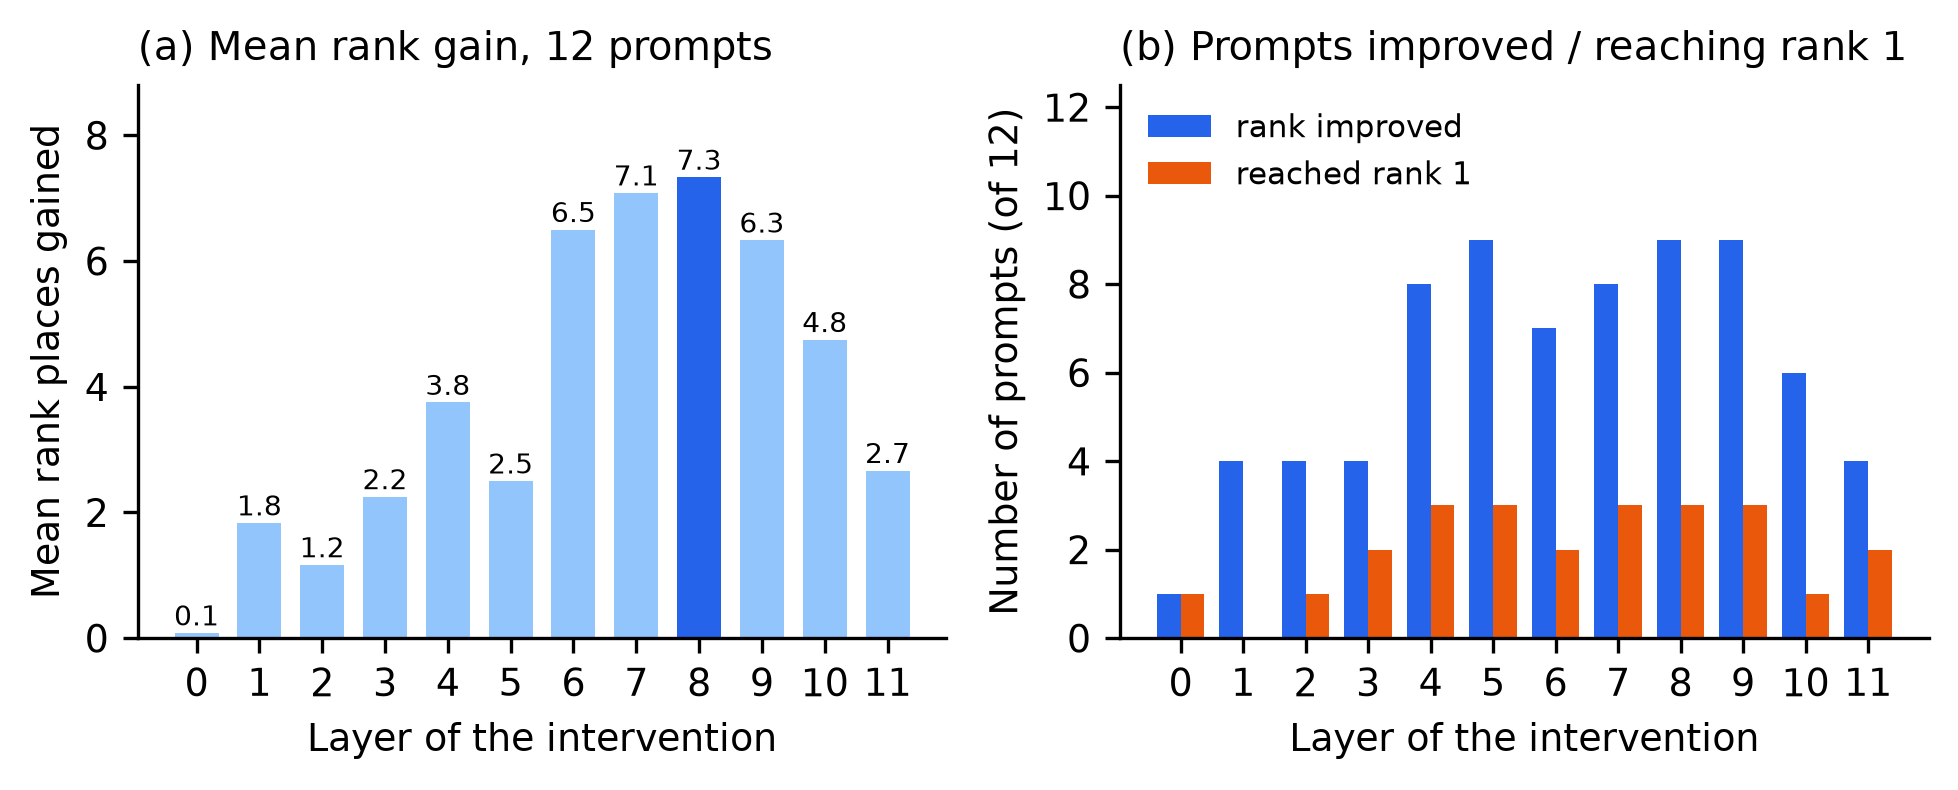
\includegraphics[width=0.92\linewidth]{figures/fig_layer12}
\caption{Layer Sweep on 12 Prompts: (a) Mean Rank Gain and (b) Prompts Improved and Prompts Reaching Rank 1, by Layer}\label{fig:layer12}
\end{figure}

An earlier run on 22 prompts at other strengths ($\mu$ = 0.5, $\beta$ = 0.7, four features on each side, layers 2, 5, 8, 10 and 11) also had its largest gains at layer 8: a mean rank gain of 4.36 and a mean probability gain of 4.84 percentage points averaged over all 22 prompts, which include 9 that were already at rank 1 and so contribute zero; over the 13 prompts that were not, the mean gain at layer 8 was 7.38, the rank improved on 11, and the target reached rank 1 on 4. The benchmark's own success flag, which counts an improvement in rank \textit{or} in probability, is not used in this report because it overstates the number of real improvements.

The data therefore show a broad plateau from layer 6 to layer 9 that falls toward both ends, with layer 8 the highest mean but not clearly separated from its neighbours on this sample, and with a different candidate mode and strengths from those of the later studies. A plausible reading is that early layers carry representations that are still too low-level for the edit to target factual content, and that late layers leave too little computation for the edit to propagate; this was not tested. It also matters that the layer was chosen by the effect of the intervention itself: Hase \textit{et al.} \cite{r30} found that where a fact is localised is a poor guide to which layer is best to edit. Layer 8 is used in all later studies as a reasonable default and not as an established optimum.

\section{Execution Cost and Platforms}\label{sec:cost}

An execution-cost audit on the RTX 4050 Laptop GPU found that both safety filters recomputed the clean baseline inside every candidate loop. Passing the precomputed baseline into the filters removed 60 passes per prompt per layer (Table~\ref{tab:passes}, Figure~\ref{fig:passes}); probabilities and ranks matched the reference to $10^{-9}$, the same mute and boost features were selected, all 60 safety decisions were identical, and the time of the safety filters was halved (Table~\ref{tab:safetyopt}). Stacking the candidates into the batch dimension of single model calls then reduced the number of model calls from 126 to 6 (21 times fewer), while the number of edited sequences evaluated stayed at 126 (Table~\ref{tab:passes}, last column). The batched ordered feature lists matched the sequential ones element by element on six prompts, and the 60 safety decisions on the canonical case again agreed.

\begin{table}[H]
\centering
\caption{Forward-Pass Accounting per Prompt per Layer}\label{tab:passes}
{\small\renewcommand{\arraystretch}{1.15}
\begin{tabular}{|>{\raggedright\arraybackslash}p{0.336\linewidth}|>{\raggedleft\arraybackslash}p{0.158\linewidth}|>{\raggedleft\arraybackslash}p{0.179\linewidth}|>{\raggedleft\arraybackslash}p{0.200\linewidth}|}
\hline
\textbf{Stage} & \textbf{Reference path} & \textbf{After Step 2} & \textbf{Batched (Step 3)} \\ \hline
1. Clean baseline & 1 & 1 & 1 \\ \hline
2. Candidate screening & 2 & 2 & 0 (clean pass cached) \\ \hline
3. Competitor causal ranking & 31 & 31 & 1 \\ \hline
4. Target causal ranking & 31 & 31 & 1 \\ \hline
5. Competitor safety filtering & 60 & 30 & 1 \\ \hline
6. Target safety filtering & 60 & 30 & 1 \\ \hline
7. Final intervention & 1 & 1 & 1 \\ \hline
\textbf{Total model calls} & \textbf{186} & \textbf{126} & \textbf{6} \\ \hline
\end{tabular}}
\end{table}

\begin{figure}[H]
\centering
\includegraphics[width=0.95\linewidth]{figures/passes}
\caption{Forward Passes by Stage before and after Optimisation}\label{fig:passes}
\end{figure}

\begin{table}[H]
\centering
\caption{Effect of Safety-Filter Optimisation (Layer 8, Cambridge, RTX 4050)}\label{tab:safetyopt}
{\small\renewcommand{\arraystretch}{1.15}
\begin{tabular}{|>{\raggedright\arraybackslash}p{0.315\linewidth}|>{\raggedleft\arraybackslash}p{0.179\linewidth}|>{\raggedleft\arraybackslash}p{0.179\linewidth}|>{\raggedleft\arraybackslash}p{0.200\linewidth}|}
\hline
\textbf{Metric} & \textbf{Reference} & \textbf{Optimised} & \textbf{Change} \\ \hline
Total forward passes & 186 & 126 & $-$32.26\% \\ \hline
Safety-filter forward passes & 120 & 60 & $-$50.00\% \\ \hline
Safety-filter time & 3,862.64 ms & 1,953.05 ms & 1.98$\times$ faster \\ \hline
Total inference time & 6.38 s & 4.39 s & $-$1.99 s \\ \hline
\end{tabular}}
\end{table}

In the application, the sequential and the batched versions of the whole Hybrid workflow took 12.16 s and 0.90 s, 11.55 s and 0.71 s, and 11.75 s and 0.58 s in three runs on one prompt, with the same result; with the batched switch on or off the model time of the Hybrid tab was about 1.0 s against 10.1 s (the hardware of these timings was not recorded). The stored layer-8 profiles show where the time went before batching: candidate selection and safety filtering together took about 97\% of the per-layer time in the 21-prompt run (Table~\ref{tab:profile}) and about 98\% in the earlier 22-prompt run (3.0 s and 5.5 s of 8.6 s).

\begin{table}[H]
\centering
\caption{Stage Timing Profile at Layer 8 before Batching (Mean over 21 Prompts, Sequential Path, 122 Model Calls; Device Not Recorded in the File)}\label{tab:profile}
{\small\renewcommand{\arraystretch}{1.15}
\begin{tabular}{|>{\raggedright\arraybackslash}p{0.539\linewidth}|>{\raggedleft\arraybackslash}p{0.389\linewidth}|}
\hline
\textbf{Stage} & \textbf{Mean time} \\ \hline
SAE loading (cached) & $<$ 0.3 ms \\ \hline
Clean baseline pass & 95 ms \\ \hline
Candidate selection (top-30) & 3,124 ms \\ \hline
Safety filtering & 3,120 ms \\ \hline
Intervention pass & 63 ms \\ \hline
\textbf{Total per layer} & \textbf{6,407 ms} \\ \hline
\end{tabular}}
\end{table}

Moving from a CPU-only PyTorch build to CUDA 12.4 made full sweeps practical. On three prompts across four layers with safety filtering enabled (about 960 forward passes), the GTX 1660 Ti completed in 150.07 s against 574.60 s on the CPU, a 3.83$\times$ speed-up (Figure~\ref{fig:gpu}). Peak GPU memory was 1,483 MB, under 25\% of the 6 GB card: about 478 MB for GPT-2 and 96 MB per SAE. The gradient-descent editor needs about 7.7 s per prompt (5.1 to 8.8 s) on the same GPU (Section~\ref{sec:gdvs}).

\begin{figure}[H]
\centering
\includegraphics[width=0.76\linewidth]{figures/gpu}
\caption{GPU versus CPU Execution Time}\label{fig:gpu}
\end{figure}

\textbf{Other platforms.} The code selects CUDA, Apple MPS or CPU automatically. The CPU path was exercised by forcing the CPU on the Windows PC: all 16 stored baseline ranks were reproduced, four gradient-descent runs gave the stored KL to four decimals, and the five additive self-checks passed. The application was also started on an Apple-silicon MacBook, where its sidebar reports MPS. MPS is asynchronous, so the timing code synchronises the device before reading the clock; without that, times would be under-measured. Timings on one device are not comparable with those on another, and all method comparisons in this report were timed on one machine. \todo{add the result of the parity check on the MacBook once it has been run}


\section{Where Candidate Features Are Drawn From}\label{sec:candsrc}

Restricting candidates to the final token can leave a small pool. For ``The leading cause of death in men is'' at layer 8, 67 features were active at the last token and 303 across all positions, and a run with pool refill used all 67 of the former (rank 152 $\rightarrow$ 50 with a limit of 10 candidates per round, and rank 51 when all 67 were used). Because scaling cannot activate a feature that is off, the number of active features bounds any edit of this kind at a single layer.

The two candidate sources were compared on 17 prompts with $\mu$ = 0.6, $\beta$ = 0.5 and $N$ = 120 at layer 8, with the safety filter and pool refill on. Three prompts already had the target at rank 1 (no edit was made in either mode) and one had a two-token target whose last piece was scored, so it is excluded. Table~\ref{tab:candsrc} and Figure~\ref{fig:candsrc} give the 13 comparable prompts. All-positions candidates reached rank 1 on 10 of 13 prompts and last-token candidates on 4 of 13. All-positions won on 9 prompts, the modes tied on 4 (both at rank 1), and last-token won on none (exact two-sided sign test on the 9 prompts that differed, $p \approx 0.004$; the prompts were chosen by the authors and are not independent draws, so this is supportive and not conclusive). The final target probability was higher with all positions on 12 of 13 prompts and identical on one. The mean number of candidate features at round 0 was 281 for all positions and 56 for the last token, and \textbf{all 9 last-token failures ended because no unapplied active feature remained}. Where both modes reached rank 1, the last token used no more features than all-positions (for example 47 against 118 on the Tesla prompt and 12 against 16 on Marie Curie). All-positions edited on average 94 features against 42 and took about twice the time (12.2 s against 5.4 s per run). Three prompts failed in both modes (Colosseum, the door prompt and ``The doctor said that''), and all-positions still ended at a better rank on each. The 34-run batch was run twice, from the application and from the command line, with identical feature lists, steps and probabilities in every run.

\begin{table}[H]
\centering
\caption{Candidate Source Study: Final Rank of the Target (Rank 1 = Reached)}\label{tab:candsrc}
{\small\renewcommand{\arraystretch}{1.15}
\begin{tabular}{|>{\raggedright\arraybackslash}p{0.431\linewidth}|>{\raggedleft\arraybackslash}p{0.119\linewidth}|>{\raggedleft\arraybackslash}p{0.162\linewidth}|>{\raggedleft\arraybackslash}p{0.162\linewidth}|}
\hline
\textbf{Prompt (target)} & \textbf{Clean} & \textbf{All positions} & \textbf{Last token} \\ \hline
This is Sophia, she is a (woman) & 6 & 1 & 2 \\ \hline
Seiyu Group's headquarters are in (Tokyo) & 2 & 1 & 1 \\ \hline
The Eiffel Tower is in the city of (Paris) & 2 & 1 & 2 \\ \hline
Marie Curie won the Nobel Prize in (Physics) & 5 & 1 & 1 \\ \hline
The Colosseum is located in (Rome) & 7 & 2 & 3 \\ \hline
Barack Obama was born in (Hawaii) & 3 & 1 & 1 \\ \hline
She opened the door and saw a (cat) & 152 & 34 & 62 \\ \hline
The programming language created by Guido van Rossum is (Python) & 44 & 1 & 4 \\ \hline
The doctor said that (she) & 3 & 2 & 3 \\ \hline
Mount Everest is located in (Nepal) & 3 & 1 & 2 \\ \hline
The CEO of Tesla is (Elon) & 335 & 1 & 1 \\ \hline
Albert Einstein was born in (Germany) & 8 & 1 & 3 \\ \hline
The largest planet in our solar system is (Jupiter) & 30 & 1 & 2 \\ \hline
\end{tabular}}
\end{table}

\begin{figure}[H]
\centering
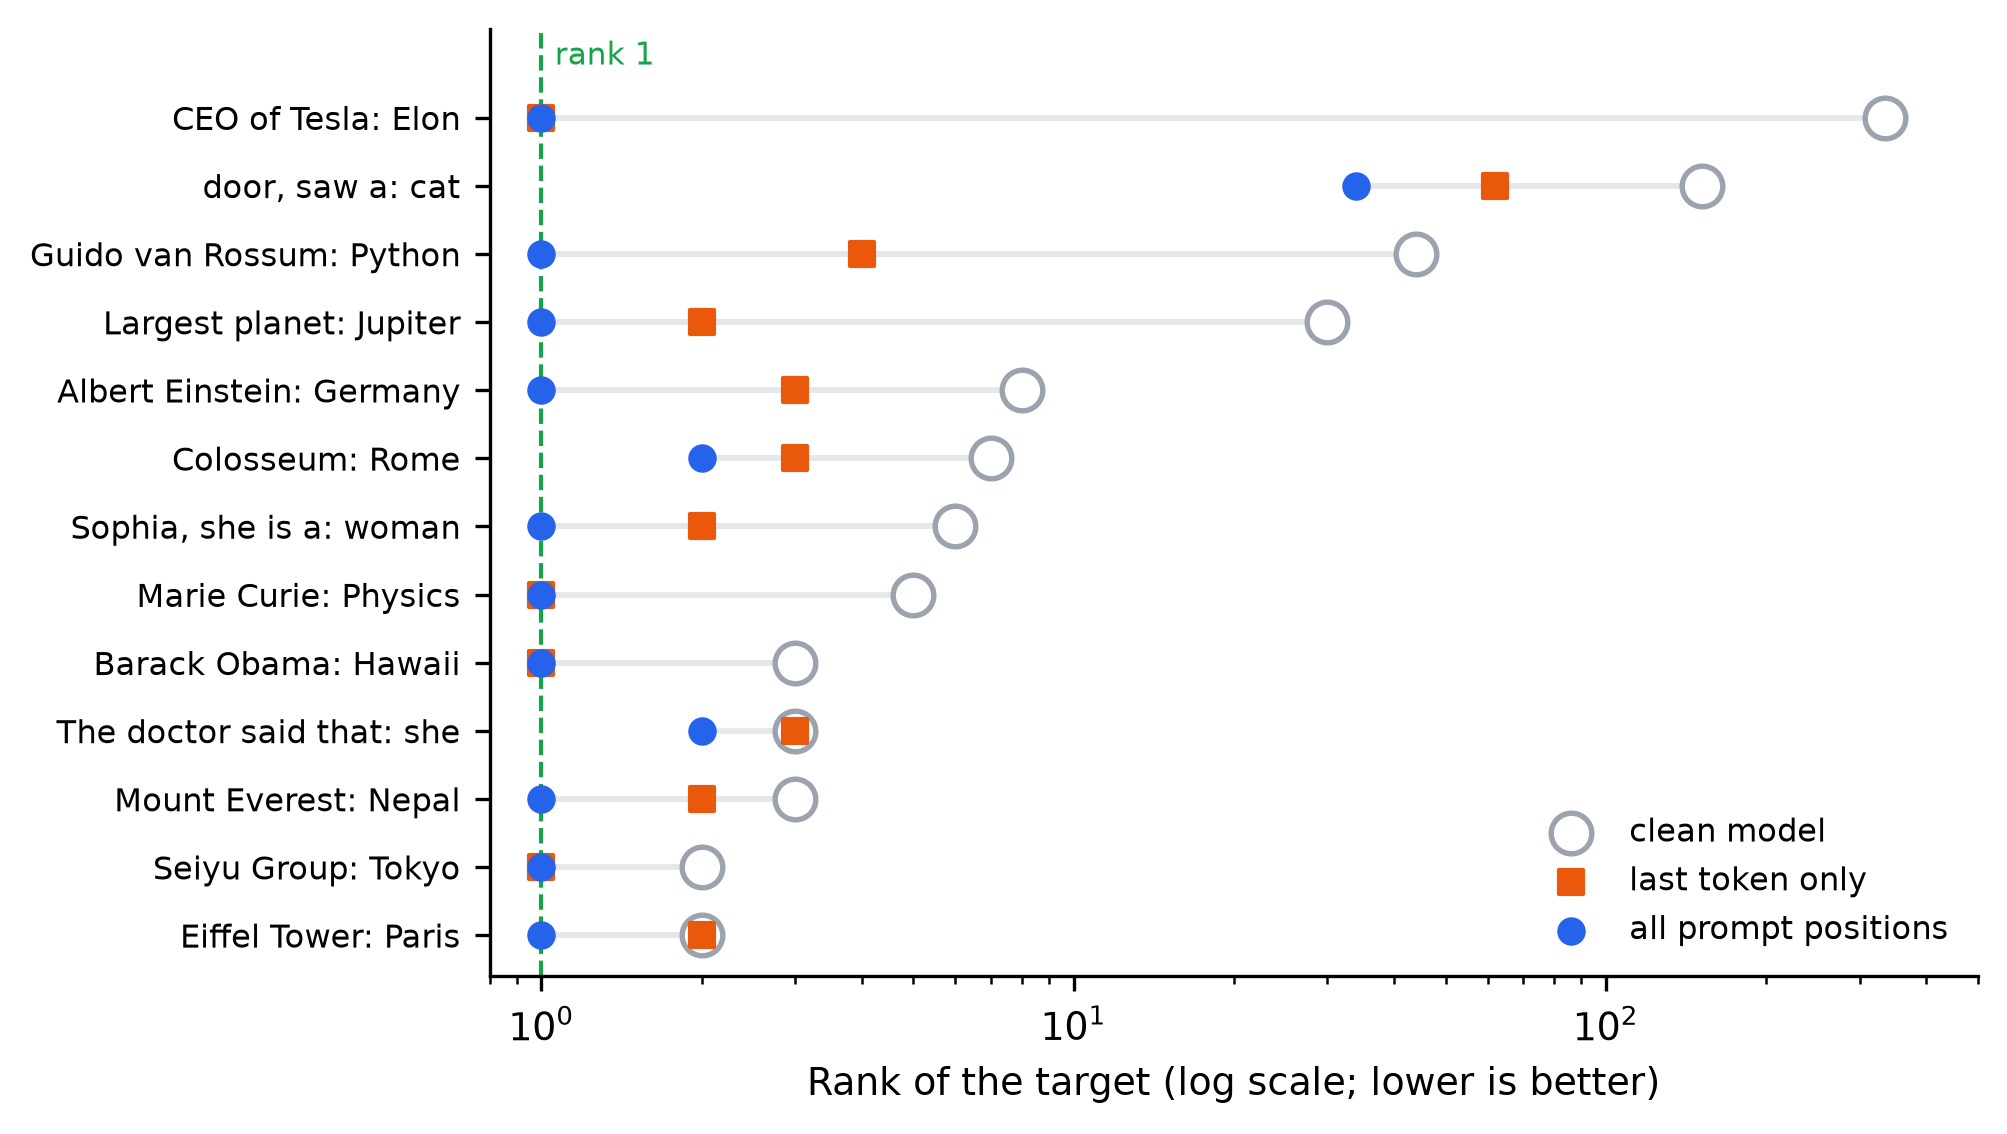
\includegraphics[width=0.88\linewidth]{figures/fig_candsrc}
\caption{Final Rank of the Target for the 13 Comparable Prompts, by Candidate Source (Log Scale)}\label{fig:candsrc}
\end{figure}

\section{Safety-Filter Study}\label{sec:filter}

The strict filter rejected roughly half of the candidates at round 0. Because rejected features are never applied, a less strict filter might have improved the outcomes. Five arms were run on identical prompts: the strict filter; no filter; a tolerance of 5\%; graded strength with the tolerance (accepted features used after the strictly safe ones); and the same graded rule with accepted features in their natural order (interleaved). Settings were $\mu$ = 0.6, $\beta$ = 0.5, $N$ = 120, pool refill on, and a limit of 250 sweep steps. Two studies were run: a pilot in all-positions mode on 45 prompts with target rank above 1 (5 controls were also run and excluded from the comparison), and a full study in last-token mode on 131 prompts. Neither study was run in the other mode. Table~\ref{tab:filterarms} and Figure~\ref{fig:filter} give the results.

\begin{table}[H]
\centering
\caption{Safety-Filter Arms. Features, Time and KL Are Means per Run; New / Lost Count Prompts That Gained or Lost Rank 1 Relative to the Strict Filter; p Is the Exact McNemar Test}\label{tab:filterarms}
{\small\renewcommand{\arraystretch}{1.15}
\begin{tabular}{|>{\raggedright\arraybackslash}p{0.161\linewidth}|>{\raggedright\arraybackslash}p{0.127\linewidth}|>{\raggedleft\arraybackslash}p{0.076\linewidth}|>{\raggedleft\arraybackslash}p{0.085\linewidth}|>{\raggedleft\arraybackslash}p{0.076\linewidth}|>{\raggedleft\arraybackslash}p{0.085\linewidth}|>{\raggedleft\arraybackslash}p{0.085\linewidth}|>{\raggedleft\arraybackslash}p{0.068\linewidth}|}
\hline
\textbf{Study} & \textbf{Arm} & \textbf{Reached} & \textbf{Features} & \textbf{Time (s)} & \textbf{KL (nats)} & \textbf{New / lost} & \textbf{p} \\ \hline
Pilot, all positions, 45 prompts & strict & 29 & 120.4 & 6.5 & 0.0055 & reference &  \\ \hline
 & no filter & 19 & 132.5 & 7.1 & 0.0069 & 0 / 10 & 0.002 \\ \hline
 & tolerance 5\% & 27 & 123.3 & 7.0 & 0.0056 & 0 / 2 & 0.50 \\ \hline
 & graded, after & 29 & 125.9 & 6.6 & 0.0054 & 0 / 0 & n/a \\ \hline
 & graded, interleaved & 29 & 125.9 & 6.6 & 0.0054 & 0 / 0 & n/a \\ \hline
Full, last token, 131 prompts & strict & 41 & 43.2 & 2.5 & 0.0015 & reference &  \\ \hline
 & no filter & 35 & 41.6 & 2.0 & 0.0014 & 4 / 10 & 0.18 \\ \hline
 & tolerance 5\% & 42 & 42.5 & 2.4 & 0.0015 & 1 / 0 & 1.0 \\ \hline
 & graded, after & 41 & 42.7 & 2.7 & 0.0014 & 0 / 0 & n/a \\ \hline
 & graded, interleaved & 41 & 42.3 & 2.6 & 0.0014 & 0 / 0 & n/a \\ \hline
\end{tabular}}
\end{table}

\begin{figure}[H]
\centering
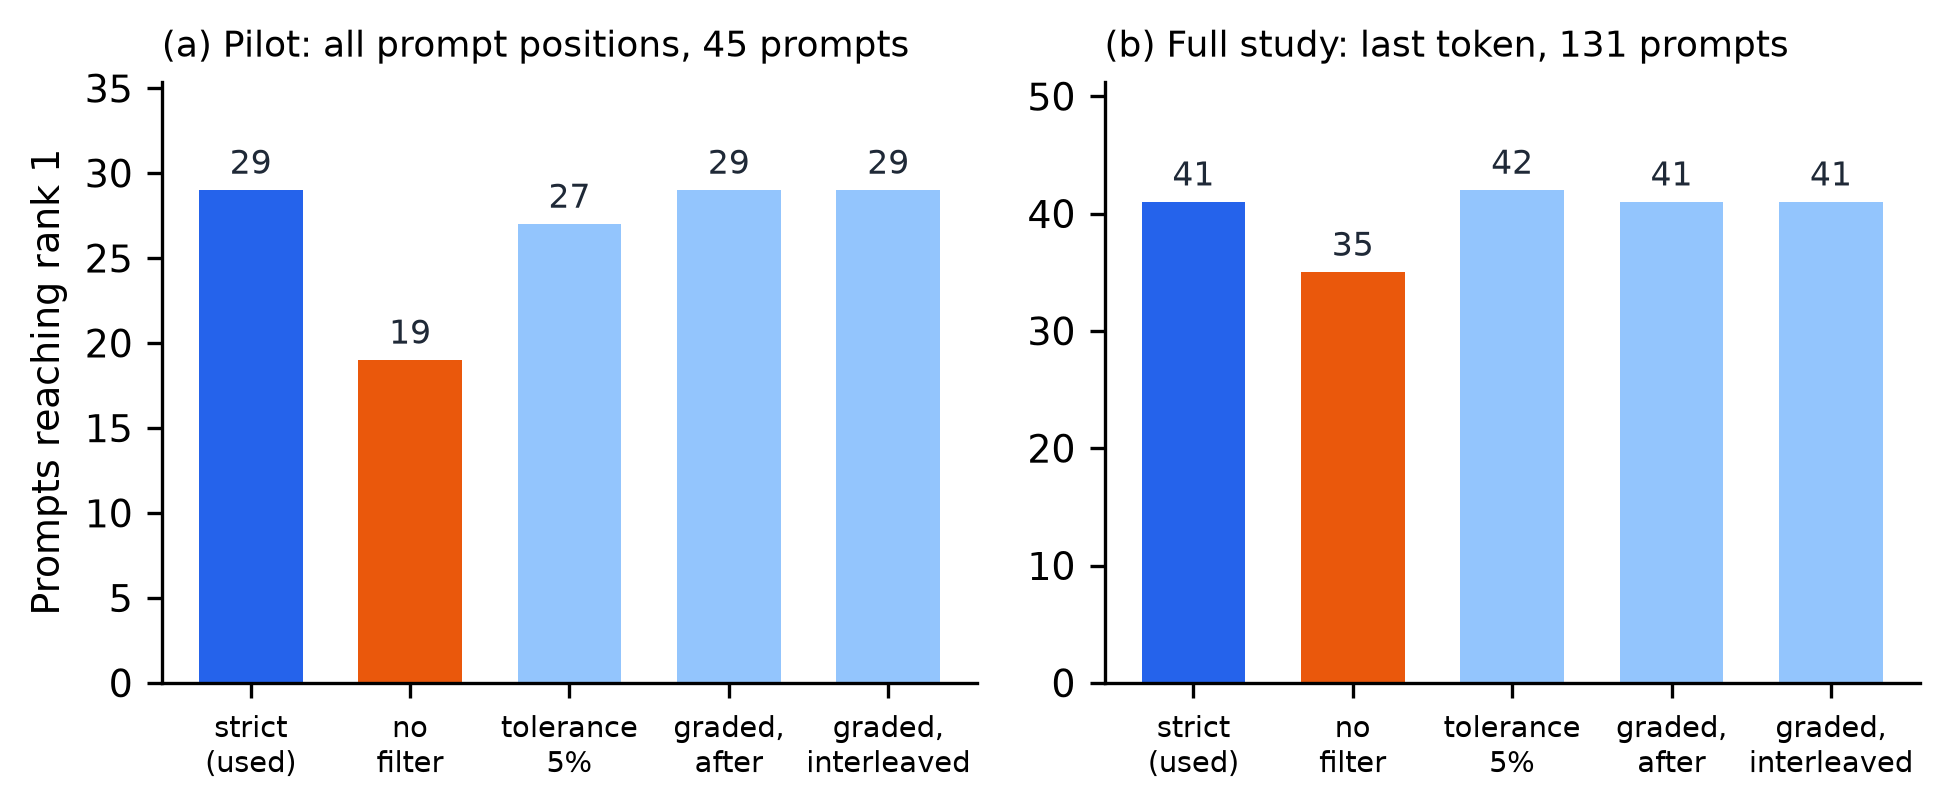
\includegraphics[width=0.95\linewidth]{figures/fig_filter}
\caption{Prompts Reaching Rank 1 under Each Safety-Filter Setting: (a) Pilot Study, 45 Prompts; (b) Full Study, 131 Prompts}\label{fig:filter}
\end{figure}

Removing the filter reduced the number of prompts reaching rank 1 from 29 to 19 of 45 in the pilot, with 10 prompts lost and none gained, and it increased the collateral KL from 0.0055 to 0.0069. In the last-token study it reached rank 1 on 35 prompts against 41, and it worsened the final rank on 64 prompts while improving it on 7. Relaxing the filter added no prompt in the pilot and at most one in the full study. Graded strength gave a worse final rank on 13 to 15 of the 131 prompts in the last-token study, and its feature counts and collateral change were close to those of the strict filter. Few rescued features were in the best result: on average 1.2 to 3.0 of about 125 features in the pilot and 0.4 to 1.1 of about 43 in the full study.

The strict filter's verdicts help explain why relaxing it changed little (Table~\ref{tab:reasons}). At round 0 about half of the candidates (mute and boost sides pooled) were accepted, and most rejections were for harm, the target probability falling by more than $10^{-6}$; 1.5 to 2.3\% failed only the rank rule and 13.9 to 15.0\% failed both. Only 157 of 5,400 candidate features (2.9\%) in the pilot and 195 of 7,691 (2.5\%) in the full study were unusable on both sides, because a feature rejected as a mute candidate is usually accepted as a boost candidate and the reverse. In the pilot, across all five arms, 83 of 250 runs ended because no unapplied active feature remained, 7 ended with no safe candidate in a round, 2 reached the step limit, 133 reached rank 1 and 25 were controls that were already at rank 1.

\begin{table}[H]
\centering
\caption{Strict-Filter Verdicts on Round-0 Candidates (Mute and Boost Sides Pooled)}\label{tab:reasons}
{\small\renewcommand{\arraystretch}{1.15}
\begin{tabular}{|>{\raggedright\arraybackslash}p{0.400\linewidth}|>{\raggedleft\arraybackslash}p{0.250\linewidth}|>{\raggedleft\arraybackslash}p{0.250\linewidth}|}
\hline
\textbf{Verdict} & \textbf{Pilot (all positions)} & \textbf{Full (last token)} \\ \hline
Accepted & 5,447 (50.4\%) & 7,776 (50.6\%) \\ \hline
Rejected, harm rule only & 3,492 (32.3\%) & 5,234 (34.0\%) \\ \hline
Rejected, rank rule only & 245 (2.3\%) & 230 (1.5\%) \\ \hline
Rejected, both rules & 1,616 (15.0\%) & 2,142 (13.9\%) \\ \hline
\end{tabular}}
\end{table}

Together with Section~\ref{sec:candsrc}, these results point to the supply of candidate features, and not to the selection rule, as the binding factor: removing the filter cost prompts, whereas relaxing it gained at most one, so the strict filter that the application uses is the one the data support. They also leave open the possibility that other limits exist.

\section{Do Later Layers Undo the Edit? Is the SAE the Limit?}\label{sec:repair}

Three worries were tested on the edit at layer 8: later layers might rebuild the removed signal (self-repair); the SAE might be more machinery than a factual edit needs; and the SAE's reconstruction error, which is never edited, might carry the information that is missing. The diagnostics ran on the three prompts that had failed in every mode of the candidate-source study (Colosseum $\rightarrow$ Rome, door $\rightarrow$ cat and ``The doctor said that'' $\rightarrow$ she) at layers 5 to 11, plus the MIT prompt at layer 8, with $N$ = 120. For each prompt and layer, the best sweep edit was converted into a residual-space delta and (1) its persistence, the projection onto the pushed direction, was traced through every later block; (2) a \textit{held edit} re-added at each later block whatever fraction of the push had been lost; and (3) an \textit{SAE-free edit}, a gradient-searched residual delta of the same size, was computed as a yardstick.

\begin{table}[H]
\centering
\caption{Repair Diagnostics: Target Rank after the SAE Edit and Persistence of the Pushed Direction at the Output, by Layer}\label{tab:repair}
{\small\renewcommand{\arraystretch}{1.15}
\begin{tabular}{|>{\raggedright\arraybackslash}p{0.277\linewidth}|>{\raggedleft\arraybackslash}p{0.069\linewidth}|>{\raggedleft\arraybackslash}p{0.069\linewidth}|>{\raggedleft\arraybackslash}p{0.069\linewidth}|>{\raggedleft\arraybackslash}p{0.069\linewidth}|>{\raggedleft\arraybackslash}p{0.069\linewidth}|>{\raggedleft\arraybackslash}p{0.069\linewidth}|>{\raggedleft\arraybackslash}p{0.069\linewidth}|}
\hline
\textbf{Prompt and measure} & \textbf{5} & \textbf{6} & \textbf{7} & \textbf{8} & \textbf{9} & \textbf{10} & \textbf{11} \\ \hline
Colosseum $\rightarrow$ Rome (clean rank 7): rank & 2 & 2 & 1 & 2 & 2 & 3 & 6 \\ \hline
Colosseum: persistence & 0.81 & 0.83 & 0.96 & 0.79 & 1.13 & 1.15 & 0.98 \\ \hline
Door $\rightarrow$ cat (clean rank 152): rank & 63 & 95 & 76 & 34 & 82 & 90 & 111 \\ \hline
Door: persistence & 0.88 & 1.16 & 1.15 & 0.91 & 1.09 & 1.15 & 1.03 \\ \hline
Doctor $\rightarrow$ she (clean rank 3): rank & 2 & 2 & 3 & 2 & 2 & 3 & 3 \\ \hline
Doctor: persistence & 0.92 & 0.93 & 0.93 & 0.90 & 1.12 & 1.21 & 1.29 \\ \hline
\end{tabular}}
\end{table}

The held edit gave the same final rank as the plain edit in all 21 layer and prompt combinations, and the pushed direction was still 0.79 to 1.29 of its injected size at the output (Table~\ref{tab:repair}), so no repair was seen. This tests only the pushed direction: a later block that rebuilds the fact along a different direction would not show as a loss of persistence, and the held-edit control cannot differ when nothing is lost, so the evidence is the persistence number. The SAE-free edit of the same size reached rank 1 in all 21 combinations, against 1 of 21 for the SAE edit (Colosseum at layer 7); the SAE-free edit needed 5 to 10\% of the residual norm on all tokens (5 to 20\% on the last token alone), whereas the SAE edits pushed 8 to 28\% of the norm and used up to 2,294 features. The SAE reconstruction error was 12 to 26\% of the activation norm and is left unedited. The logit-lens margin of the target \cite{r37} was negative at every block for all four prompts. On the MIT prompt at layer 8 the SAE edit reached rank 1 with 22 features.

\textbf{Scope.} These counts are over layer and prompt combinations on three prompts that were chosen because the SAE method had already failed on them, so they are not success rates and cannot be compared with those of the other sections. The SAE-free edit is an upper bound optimised for the target alone, probably a damaging edit; its side effects were not measured. What the diagnostics do support is that the failures were not caused by the layer or by later-layer repair, and that the multi-layer intervention considered at one point is not motivated by repair.

\section{The CounterFact Benchmark and the Headroom of Feature Scaling}\label{sec:headroom}

Before any method for choosing strengths was built, a headroom measurement asked how far any choice of multipliers could go. Using only the per-prompt cache, an edit $\sum_k (m_k - 1) A_k W_{\text{dec}}[k]$ was added to the saved layer-8 state and only blocks 8 to 11 were run (about 50 ms per try; a batch of 32 prompts costs the same as one). For each of the 1,450 cached prompts, 100 gradient steps tuned free multipliers in $[0,3]$ for the 200 candidates (``SAE multipliers''), with and without a penalty on side effects, and a free direction in the residual stream of a fixed size (``free push'') served as a yardstick. The edit evaluation was validated against the real hook: the same random edit on 12 prompts gave outputs within $8.8\times10^{-6}$ and the same target rank on 12 of 12.

\begin{table}[H]
\centering
\caption{Headroom Measurement on the 1,450 Cached Prompts (One-Shot Edits on Saved Layer-8 States; a Stand-in for the Real Sweep)}\label{tab:headroom}
{\small\renewcommand{\arraystretch}{1.15}
\begin{tabular}{|>{\raggedright\arraybackslash}p{0.376\linewidth}|>{\raggedleft\arraybackslash}p{0.199\linewidth}|>{\raggedleft\arraybackslash}p{0.144\linewidth}|>{\raggedleft\arraybackslash}p{0.155\linewidth}|}
\hline
\textbf{Method} & \textbf{Reaching rank 1} & \textbf{Mean KL (nats)} & \textbf{Mean edit size} \\ \hline
SAE multipliers, no damage limit & 1,158 (80\%) & 1.036 & 35.7\% \\ \hline
SAE multipliers, side effects penalised & 592 (41\%) & 0.056 & 19.4\% \\ \hline
SAE fixed rule, top 5 mute / boost & 89 (6\%) & 0.070 & 12.4\% \\ \hline
SAE fixed rule, top 20 & 169 (12\%) & 0.146 & 14.9\% \\ \hline
SAE fixed rule, top 50 & 218 (15\%) & 0.198 & 16.1\% \\ \hline
Free push, last token, 5\% of norm & 254 (18\%) & 0.066 & 5.0\% \\ \hline
Free push, last token, 10\% & 683 (47\%) & 0.231 & 10.0\% \\ \hline
Free push, last token, 20\% & 1,432 (99\%) & 0.871 & 20.0\% \\ \hline
Free push, all tokens, 5\% & 844 (58\%) & 0.270 & 5.4\% \\ \hline
Free push, all tokens, 10\% & 1,441 (99\%) & 1.106 & 11.1\% \\ \hline
Free push, all tokens, 20\% & 1,450 (100\%) & 2.439 & 23.6\% \\ \hline
\end{tabular}}
\end{table}

\begin{figure}[H]
\centering
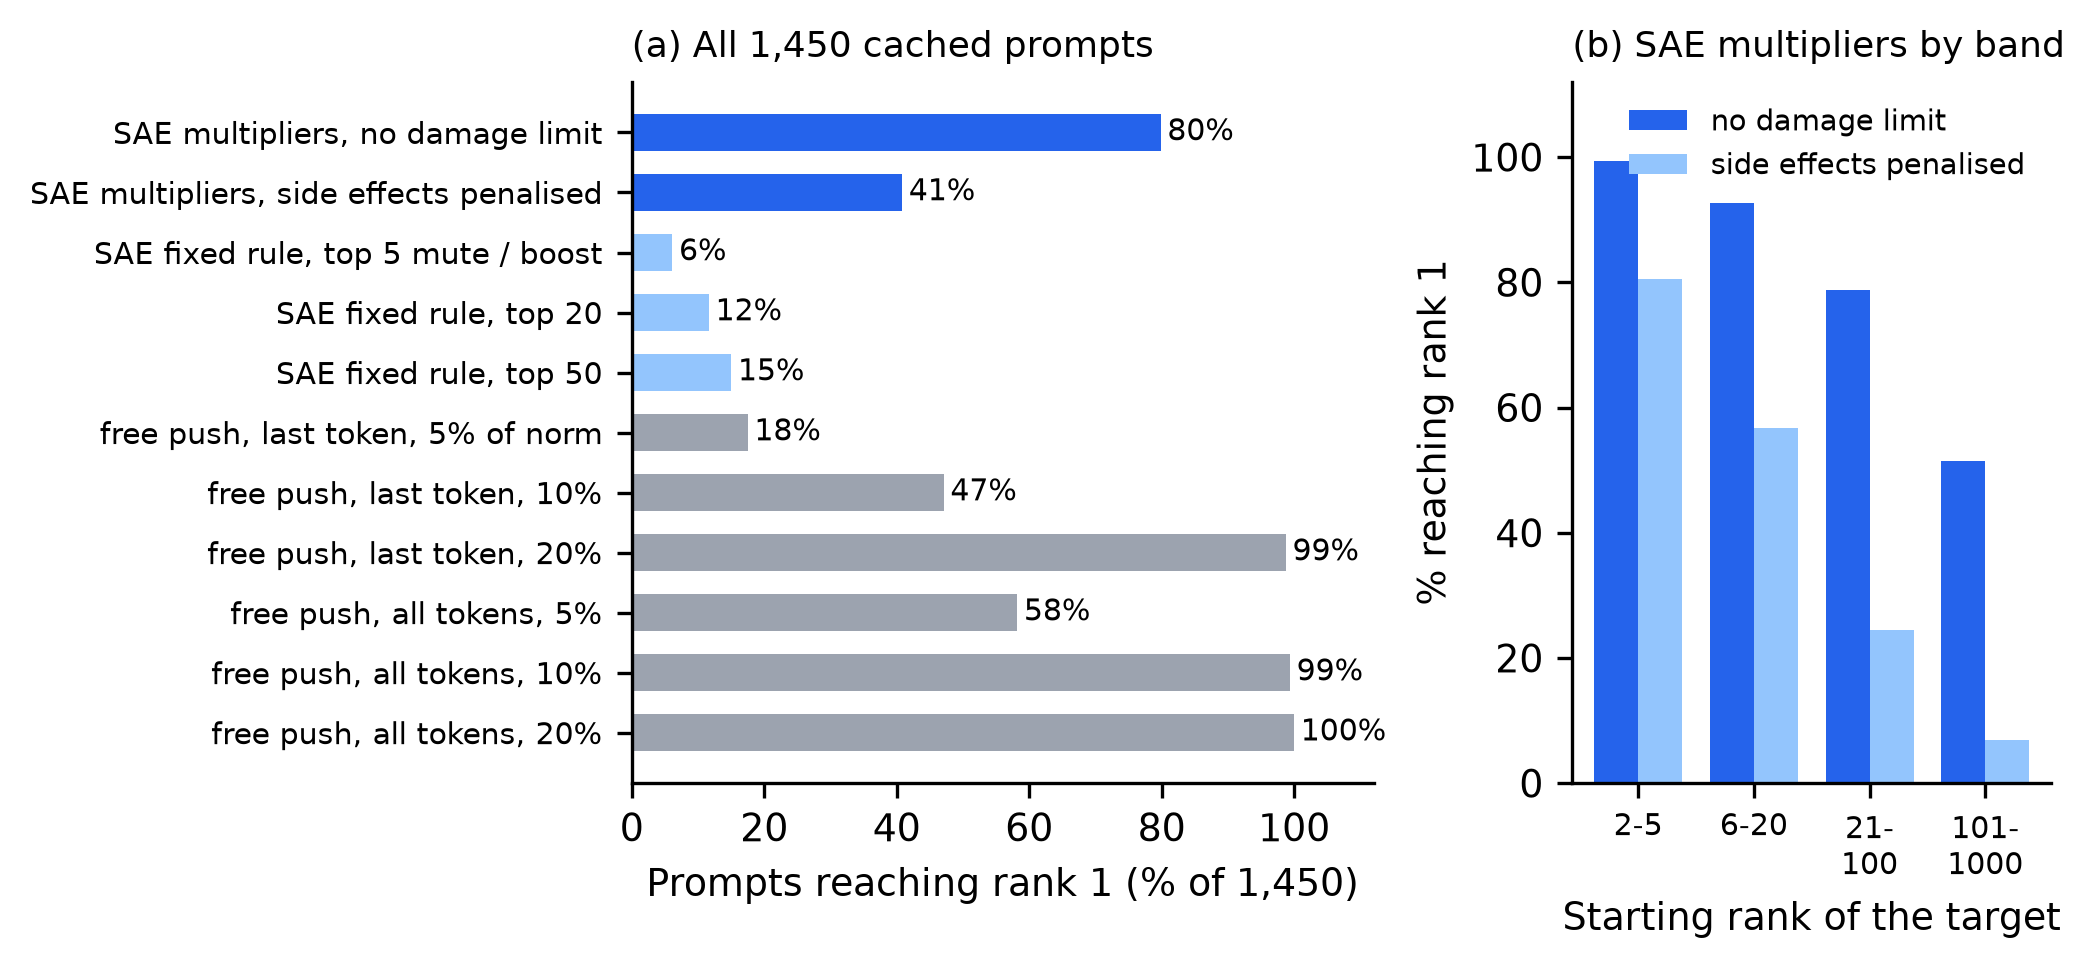
\includegraphics[width=0.98\linewidth]{figures/fig_headroom}
\caption{Headroom Measurement: (a) Share of the 1,450 Cached Prompts Reaching Rank 1 by Method; (b) SAE Multipliers by Starting-Rank Band}\label{fig:headroom}
\end{figure}

As Table~\ref{tab:headroom} and Figure~\ref{fig:headroom} show, scaling SAE features could in principle bring the target to rank 1 on about 80\% of the prompts if side effects are ignored, and on 41\% with one particular setting of a side-effect penalty, against 6 to 15\% for the crude fixed rules; the shares were the same on the training, validation and both test sets (79 to 85\% for the unpenalised case), so the split does not drive the ceiling. Prompts that start deep (rank 101 to 1000) were reachable only about half the time without a damage limit (194 of 377, 51\%) and on 26 of 377 (7\%) with the penalty. The limits of this measurement matter. It is a one-shot edit on a saved state, not the real sweep (no safety filter, no step-by-step addition, no refill); the 41\% depends on the arbitrary penalty weights (side-effect weight 20, size weight 0.01) and illustrates a trade-off and not a bound; the free pushes were optimised without any side-effect penalty, so their KL values are not comparable with those of the penalised SAE edit, and no equal-damage comparison between SAE edits and free pushes has been made.

\section{Learned Mute and Boost Strengths}\label{sec:learned}

The fixed strengths of the sweep (mute 0.6, boost 0.5) are the same for every prompt, although experience showed that the strengths change the outcome. Three ways of choosing them were compared with the fixed pair: a \textit{learned fixed pair} (two numbers shared by all prompts, trained by the same method), \textit{PromptNet} (a small network that maps 12 summary numbers about the prompt, such as the target's rank and probability, to one mute and one boost strength), and a \textit{per-prompt tuned} value found by gradient descent on each evaluation prompt, which is the best that a network could hope to approximate. Training used gradients through blocks 8 to 11 from the cached states, with a stand-in for the sweep that applies growing prefixes of the allowed features. \textbf{All numbers in this section are from that stand-in measure; the real sweep was never run with these strengths.}

\begin{table}[H]
\centering
\caption{Prompts Reaching Rank 1 under the Stand-in Measure (Count and Share of the Set)}\label{tab:learnedcounts}
{\small\renewcommand{\arraystretch}{1.15}
\begin{tabular}{|>{\raggedright\arraybackslash}p{0.230\linewidth}|>{\raggedleft\arraybackslash}p{0.134\linewidth}|>{\raggedleft\arraybackslash}p{0.154\linewidth}|>{\raggedleft\arraybackslash}p{0.154\linewidth}|>{\raggedleft\arraybackslash}p{0.173\linewidth}|}
\hline
\textbf{Set (prompts)} & \textbf{Fixed 0.6 / 0.5} & \textbf{Learned fixed pair} & \textbf{PromptNet} & \textbf{Per-prompt tuned} \\ \hline
Validation (150) & 38 (25.3\%) & 62 (41.3\%) & 63 (42.0\%) & 66 (44.0\%) \\ \hline
Test, seen relations (150) & 33 (22.0\%) & 56 (37.3\%) & 58 (38.7\%) & 58 (38.7\%) \\ \hline
Test, unseen relations (150) & 42 (28.0\%) & 60 (40.0\%) & 61 (40.7\%) & 65 (43.3\%) \\ \hline
\textbf{Test, both (300)} & \textbf{75 (25.0\%)} & \textbf{116 (38.7\%)} & \textbf{119 (39.7\%)} & \textbf{123 (41.0\%)} \\ \hline
\end{tabular}}
\end{table}

\begin{figure}[H]
\centering
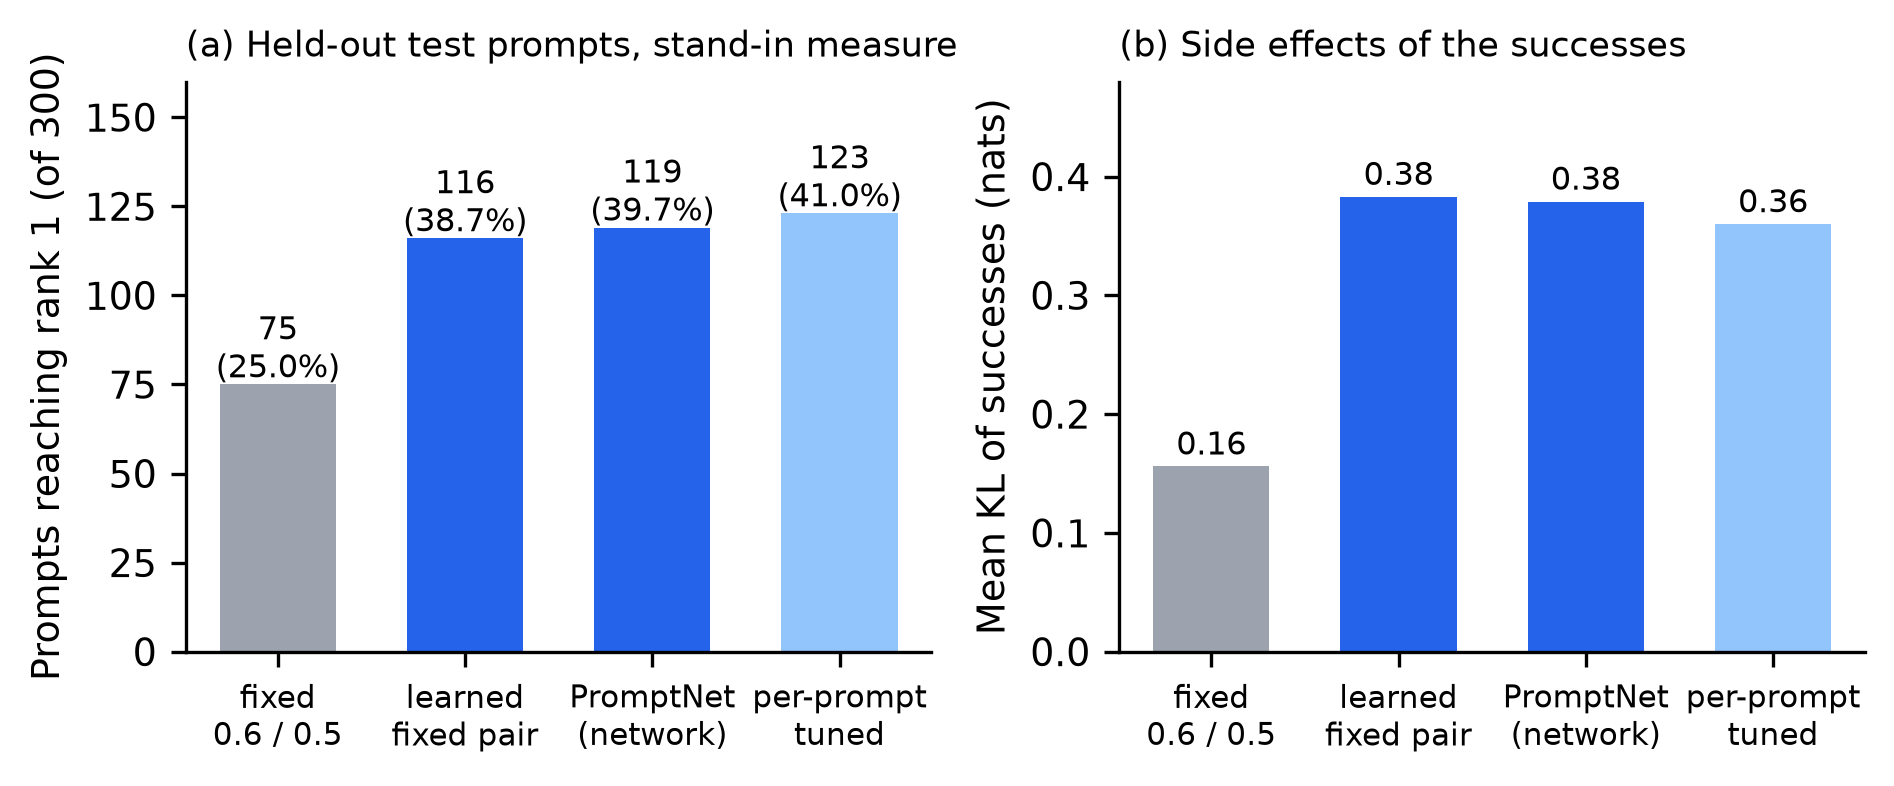
\includegraphics[width=0.92\linewidth]{figures/fig_learned}
\caption{Learned Strengths on the 300 Held-Out Test Prompts (Stand-in Measure): (a) Prompts Reaching Rank 1; (b) Mean KL of the Successes}\label{fig:learned}
\end{figure}

Table~\ref{tab:learnedcounts} and Figure~\ref{fig:learned} give the counts. On the 300 test prompts (validation, used for early stopping, is excluded) the learned fixed pair, with mute 0.98 and boost 1.81, fixed 42 prompts that the reference did not and lost 1 (exact McNemar $p < 0.0001$). PromptNet reached 3 prompts more than the pair and none fewer ($p = 0.25$), and the per-prompt tuned value 12 more and 5 fewer than the pair ($p = 0.14$). The learning curve was flat from 100 training prompts on. The better pair roughly doubled the side effects of the successes (mean KL 0.156 for the reference, 0.383 for the pair, 0.379 for PromptNet, 0.360 for the per-prompt value), which depends on the side-effect weight chosen for training. Prompts that start at rank 101 to 1000 stayed almost unfixable under every choice (on all 450 held-out prompts, 1 of 117 for the reference, 6 of 117 for the pair and 8 of 117 for the per-prompt value).

A second version gave every candidate feature its own multiplier through a small shared network (FeatureNet). In development runs (one seed, 500 training prompts, one-shot stand-in) it reached about 31 to 32\% of the held-out prompts, below the pair (about 37\% on the same stand-in) and far below the 73.3\% reached by free per-feature multipliers tuned on each prompt; its full run was not made.

The finding is therefore \textbf{a better global default}, about mute 0.98 and boost 1.8 in place of 0.6 and 0.5, and not a benefit of choosing per prompt. The large gap between free per-feature multipliers (73\%) and the per-pool bound (about 40\%) is what motivated the gradient-descent editor of the next section.


\section{Gradient Descent against the Sweep}\label{sec:gdvs}

Hand trials in the Hybrid tab on nine prompts chosen by the authors (Appendix~B.4) suggested that giving every candidate feature its own multiplier gets nearer to rank 1 than the fixed sweep. On the six prompts where both methods were run, gradient descent ended nearer to rank 1 every time and reached rank 1 on three (``The sky is'' $\rightarrow$ black, ``Frankie Lee Sims died at'' $\rightarrow$ Dallas, ``Kaka professionally plays the sport'' $\rightarrow$ soccer), where the sweep reached none; targets that are not plausible answers (a random name, ``Adi'', or ``rapist'' after ``My nephew is a'') reached rank 1 under neither method. These trials were confounded: gradient descent could scale a feature anywhere from 0 to 3 times, whereas the sweep at the strengths used reached only about 0.4 to 1.8 times, and the side effects of the sweep had never been measured. The controlled comparison below removes both confounds.

\textbf{Setup.} The 300 held-out test prompts of the hard set were used (150 with seen and 150 with unseen relations; starting-rank bands 2--5: 67 prompts, 6--20: 76, 21--100: 78, 101--1000: 79), with the true answer, a single GPT-2 token, as target, $N$ = 200 candidates from all prompt positions, on the GTX 1660 Ti, and the real model throughout (not the stand-in of the previous sections). Three arms were run: the real sweep as in the application (cumulative, unlimited pool refill, strict filter, combination check) at mute 0.6 and boost 0.5, which reaches 0.4 to 1.5 times per feature; the same sweep at mute 1.0 and boost 2.0, which reaches 0 to 3 times and so has the same allowed range as gradient descent; and gradient descent with the settings of Table~\ref{tab:gdsettings}. One yardstick was applied to every arm: the arm's final edit (the sweep's best step, or the iterate kept by gradient descent) was turned into a per-feature scale map and applied through the real hook, and rank, probability, same-prompt KL, features changed (multiplier more than 0.05 from 1), edit size, KL and top-1 flips on the 20 unrelated prompts, and model-compute time were measured. The sweep's own reported best rank equalled the re-measured rank on every prompt, so its final edits were reproduced exactly. Table~\ref{tab:gdvs} gives the totals.

\begin{table}[H]
\centering
\caption{Equal-Budget Comparison on the 300 Held-Out Prompts (Real Model)}\label{tab:gdvs}
{\small\renewcommand{\arraystretch}{1.15}
\begin{tabular}{|>{\raggedright\arraybackslash}p{0.163\linewidth}|>{\raggedleft\arraybackslash}p{0.126\linewidth}|>{\raggedleft\arraybackslash}p{0.089\linewidth}|>{\raggedleft\arraybackslash}p{0.081\linewidth}|>{\raggedleft\arraybackslash}p{0.074\linewidth}|>{\raggedleft\arraybackslash}p{0.089\linewidth}|>{\raggedleft\arraybackslash}p{0.067\linewidth}|>{\raggedleft\arraybackslash}p{0.074\linewidth}|}
\hline
\textbf{Arm} & \textbf{Reached rank 1} & \textbf{Median KL} & \textbf{Features changed} & \textbf{Edit size} & \textbf{Unrelated-prompt KL} & \textbf{Top-1 flips} & \textbf{Time (mean)} \\ \hline
Sweep, mute 0.6 / boost 0.5 & 94 (31.3\%) & 0.259 & 247 & 0.176 & 0.0045 & 0.05 & 49.7 s \\ \hline
Sweep, mute 1.0 / boost 2.0 & 161 (53.7\%) & 0.600 & 182 & 0.408 & 0.0292 & 0.08 & 38.5 s \\ \hline
\textbf{Gradient descent} & \textbf{271 (90.3\%)} & \textbf{0.144} & 193 & 0.217 & 0.0088 & 0.06 & \textbf{7.7 s} \\ \hline
\end{tabular}}
\end{table}

Median KL is the same-prompt KL over all prompts of the arm, including those that failed; the sweeps succeed on different (easier) sets of prompts, so the paired comparison below and not the mean KL of successes is the fair one. The paired tests give the following. For reaching rank 1, gradient descent solved 177 prompts that the original sweep did not and lost none ($p = 10^{-53}$), and 110 that the wide sweep did not and lost none ($p = 2\times10^{-33}$); the wide sweep solved 68 that the original sweep did not and lost one ($p = 2\times10^{-19}$). On the prompts that two arms both solved, the same-prompt KL of gradient descent was lower on 92 of 94 against the original sweep (median difference 0.095, Wilcoxon $p = 6\times10^{-17}$) and on 160 of 161 against the wide sweep (median difference 0.331, $p = 10^{-27}$). By starting-rank band (Table~\ref{tab:gdbands}, Figure~\ref{fig:gd1}), gradient descent solved every prompt in the two easiest bands, 74 of 78 in the third, and 54 of 79 in the hardest, where its success probabilities are also smallest (median 4.9\%).

\begin{table}[H]
\centering
\caption{Prompts Reaching Rank 1 by Starting-Rank Band, and Median Same-Prompt KL}\label{tab:gdbands}
{\small\renewcommand{\arraystretch}{1.15}
\begin{tabular}{|>{\raggedright\arraybackslash}p{0.136\linewidth}|>{\raggedleft\arraybackslash}p{0.109\linewidth}|>{\raggedleft\arraybackslash}p{0.109\linewidth}|>{\raggedleft\arraybackslash}p{0.127\linewidth}|>{\raggedleft\arraybackslash}p{0.200\linewidth}|>{\raggedleft\arraybackslash}p{0.136\linewidth}|}
\hline
\textbf{Band (prompts)} & \textbf{Sweep 0.6 / 0.5} & \textbf{Sweep 1.0 / 2.0} & \textbf{Gradient descent} & \textbf{Median KL (sweep, wide sweep, gradient descent)} & \textbf{Gradient descent: median target probability of its successes} \\ \hline
2--5 (67) & 51 & 63 & 67 & 0.11 / 0.21 / 0.02 & 9.7\% \\ \hline
6--20 (76) & 31 & 54 & 76 & 0.25 / 0.49 / 0.08 & 8.5\% \\ \hline
21--100 (78) & 10 & 31 & 74 & 0.31 / 0.75 / 0.29 & 7.6\% \\ \hline
101--1000 (79) & 2 & 13 & 54 & 0.35 / 0.83 / 0.55 & 4.9\% \\ \hline
\end{tabular}}
\end{table}

\begin{figure}[H]
\centering
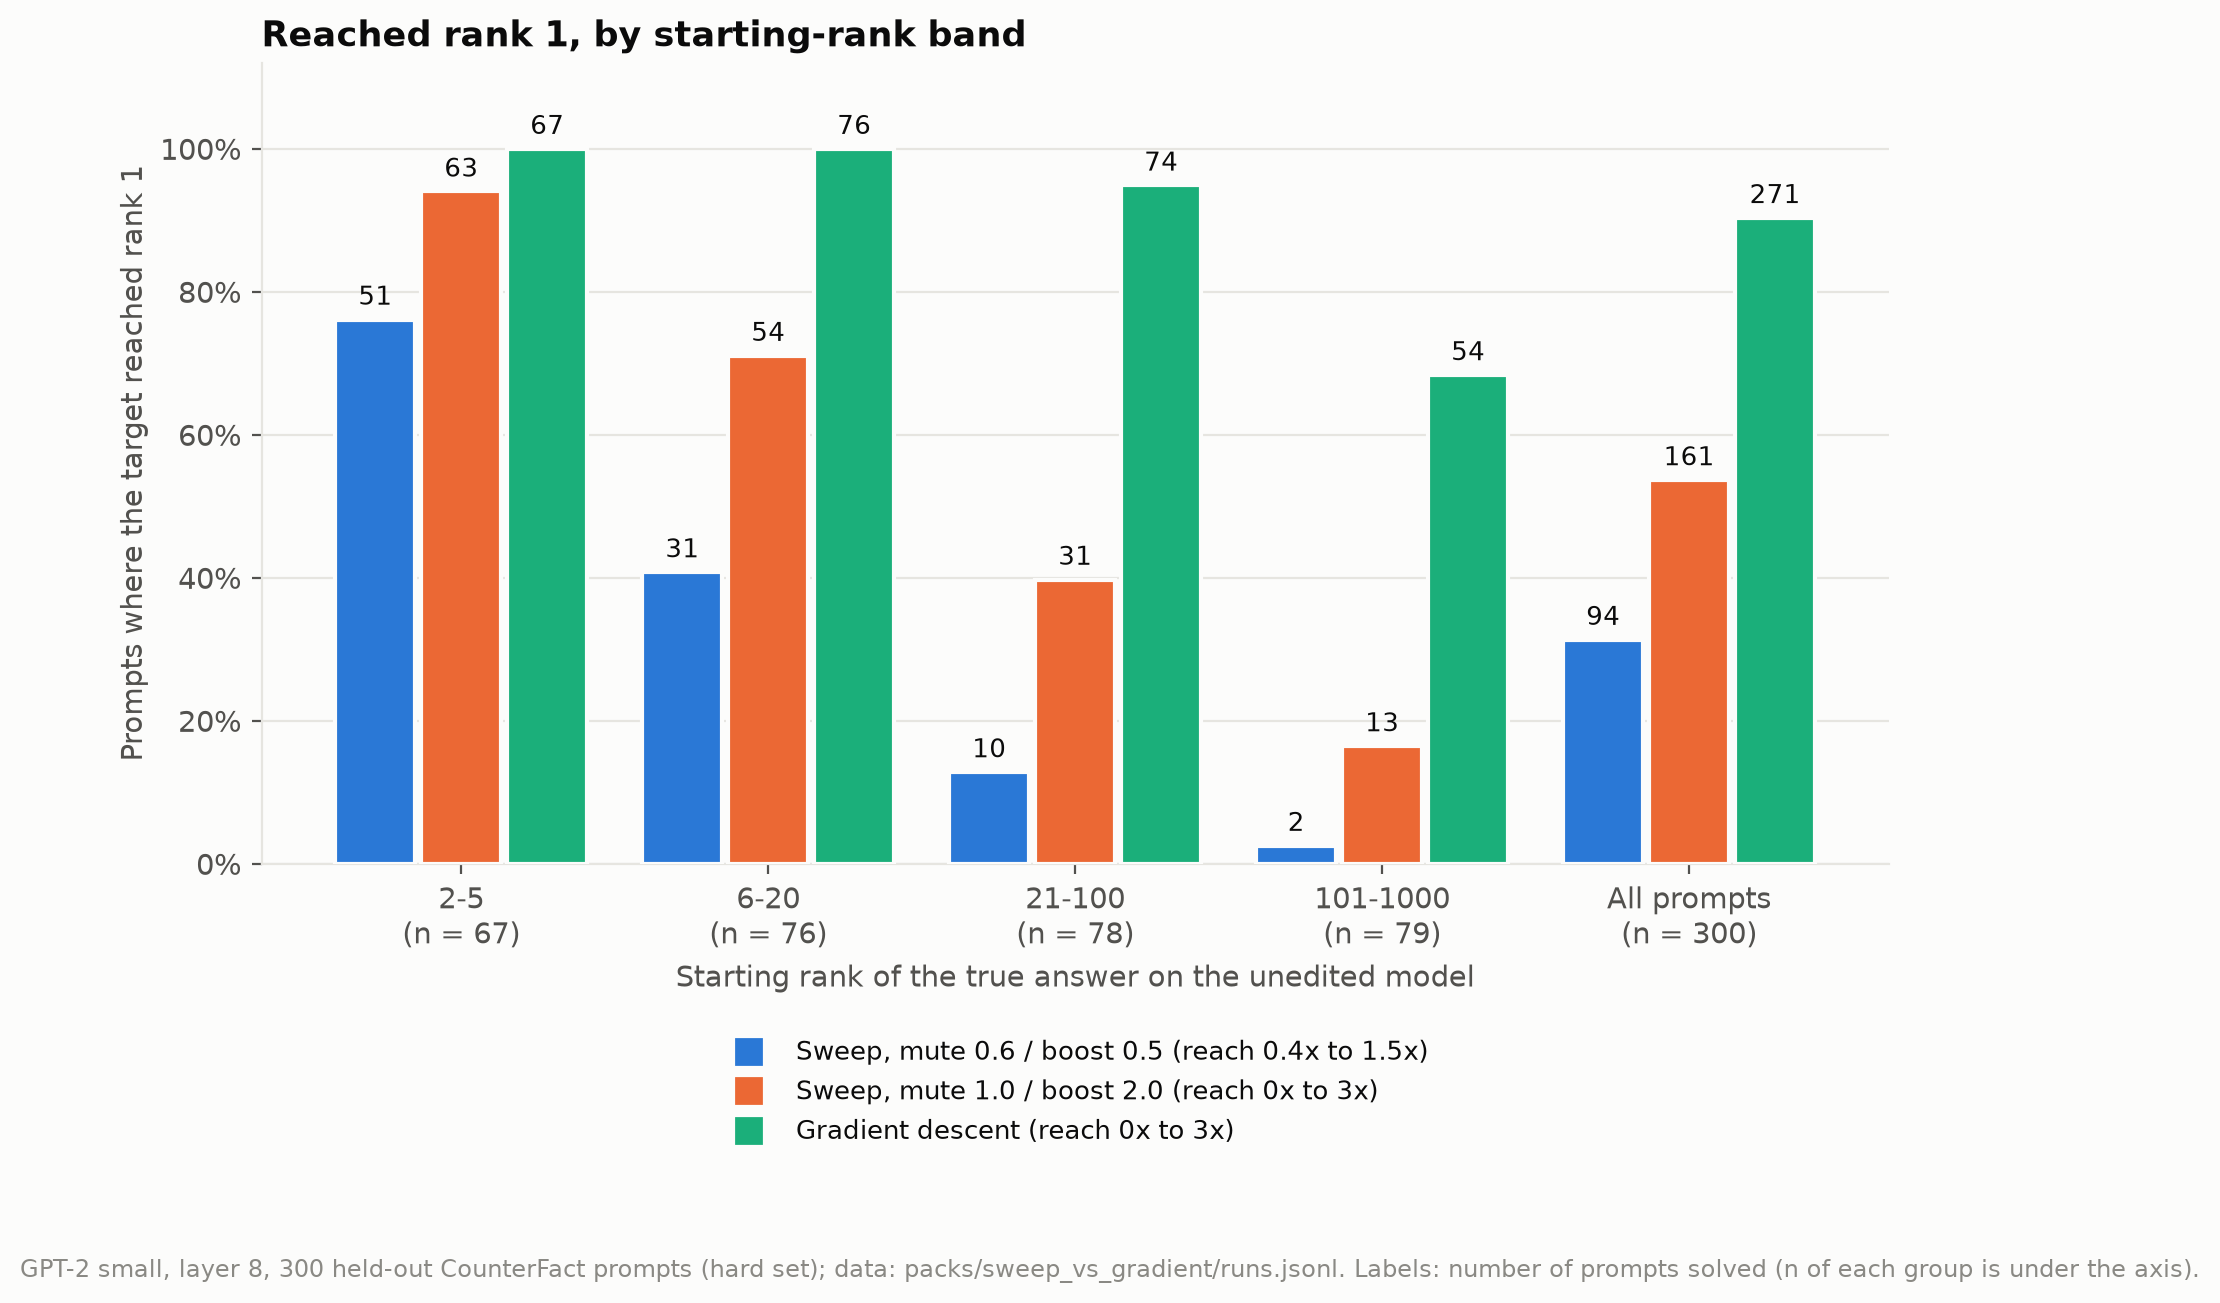
\includegraphics[width=0.92\linewidth]{figures/gd_rank1_by_band}
\caption{Prompts Reaching Rank 1 by Starting-Rank Band: the Two Sweeps and Gradient Descent (300 Held-Out Prompts)}\label{fig:gd1}
\end{figure}

\begin{figure}[H]
\centering
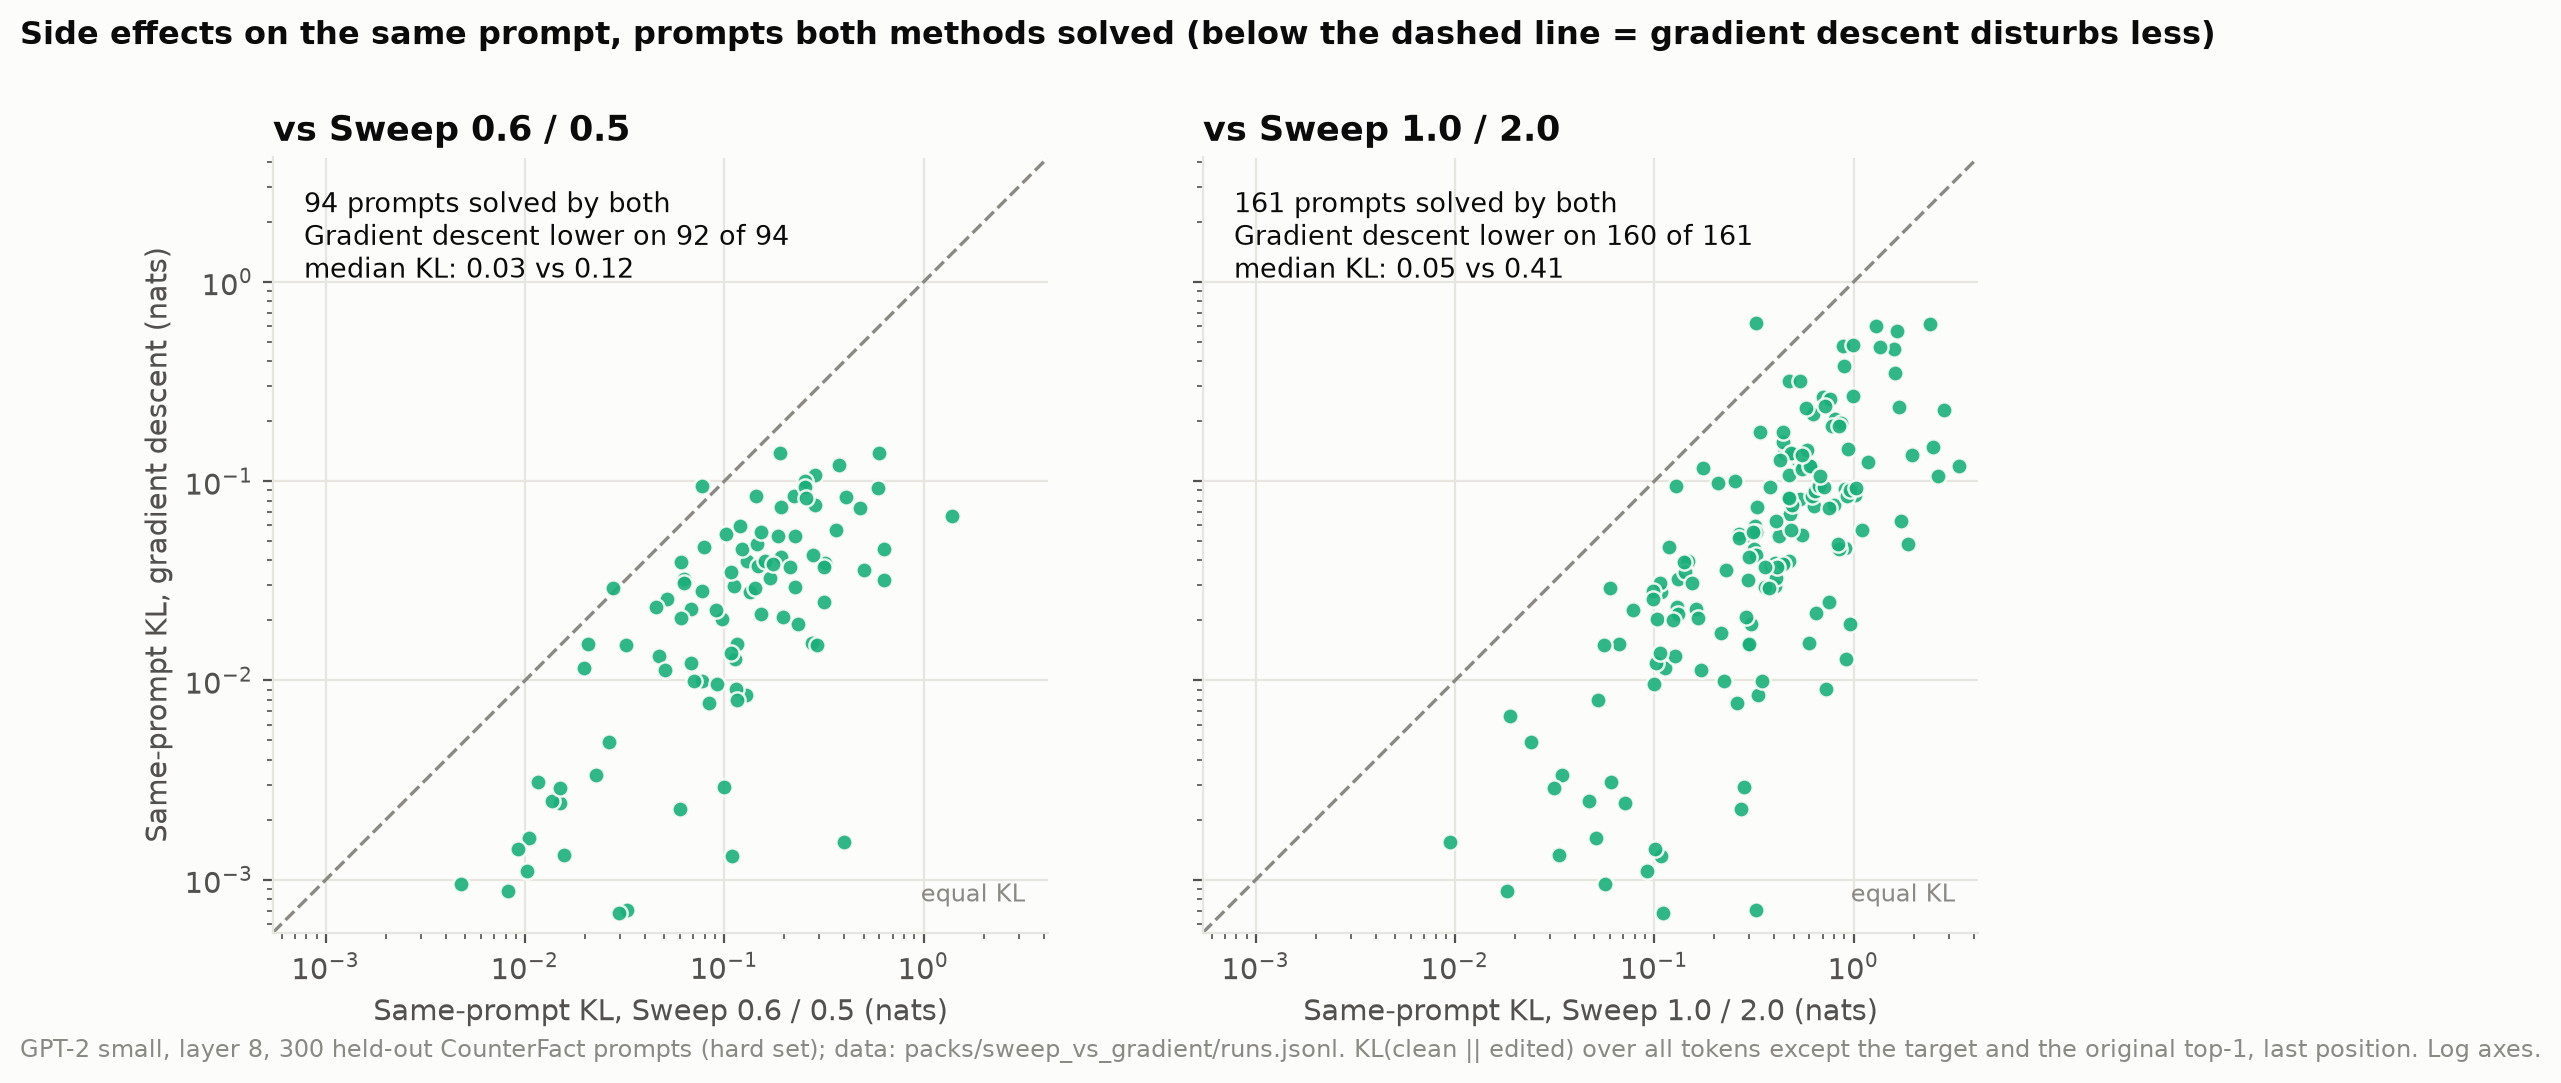
\includegraphics[width=0.98\linewidth]{figures/gd_kl_paired}
\caption{Same-Prompt Side Effects (KL) on the Prompts that Both Methods Solved; a Point below the Dashed Line Means Gradient Descent Disturbs the Output Less}\label{fig:gd2}
\end{figure}

\begin{figure}[H]
\centering
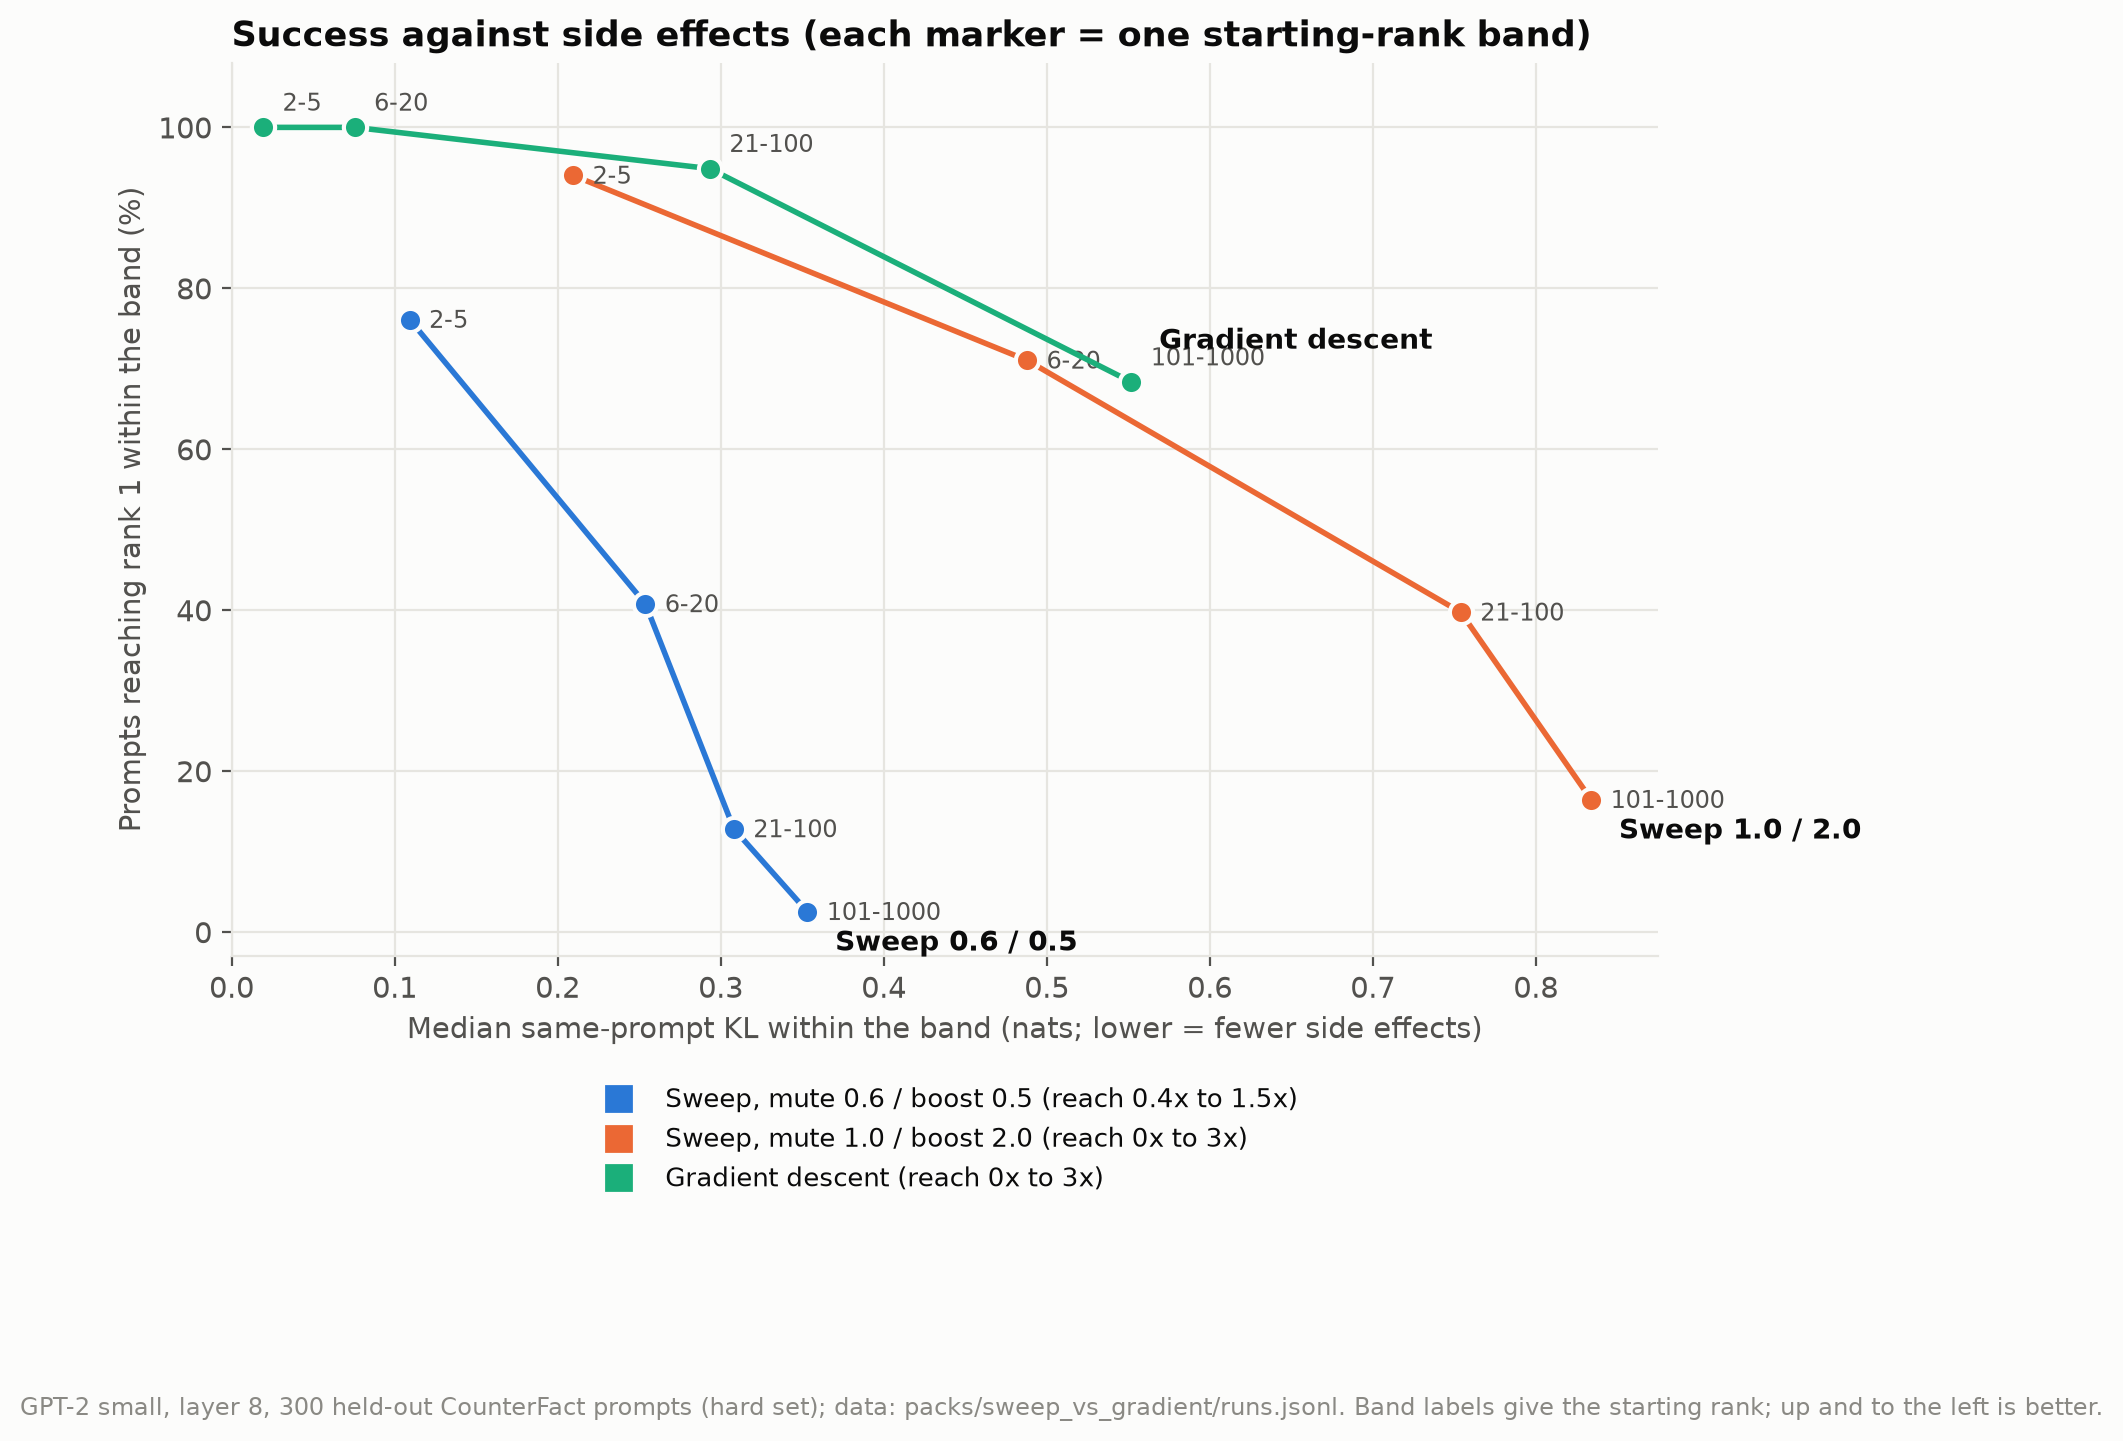
\includegraphics[width=0.85\linewidth]{figures/gd_success_vs_kl}
\caption{Success against Side Effects: Each Marker Is One Starting-Rank Band for One Method (Up and to the Left Is Better)}\label{fig:gd3}
\end{figure}

\begin{figure}[H]
\centering
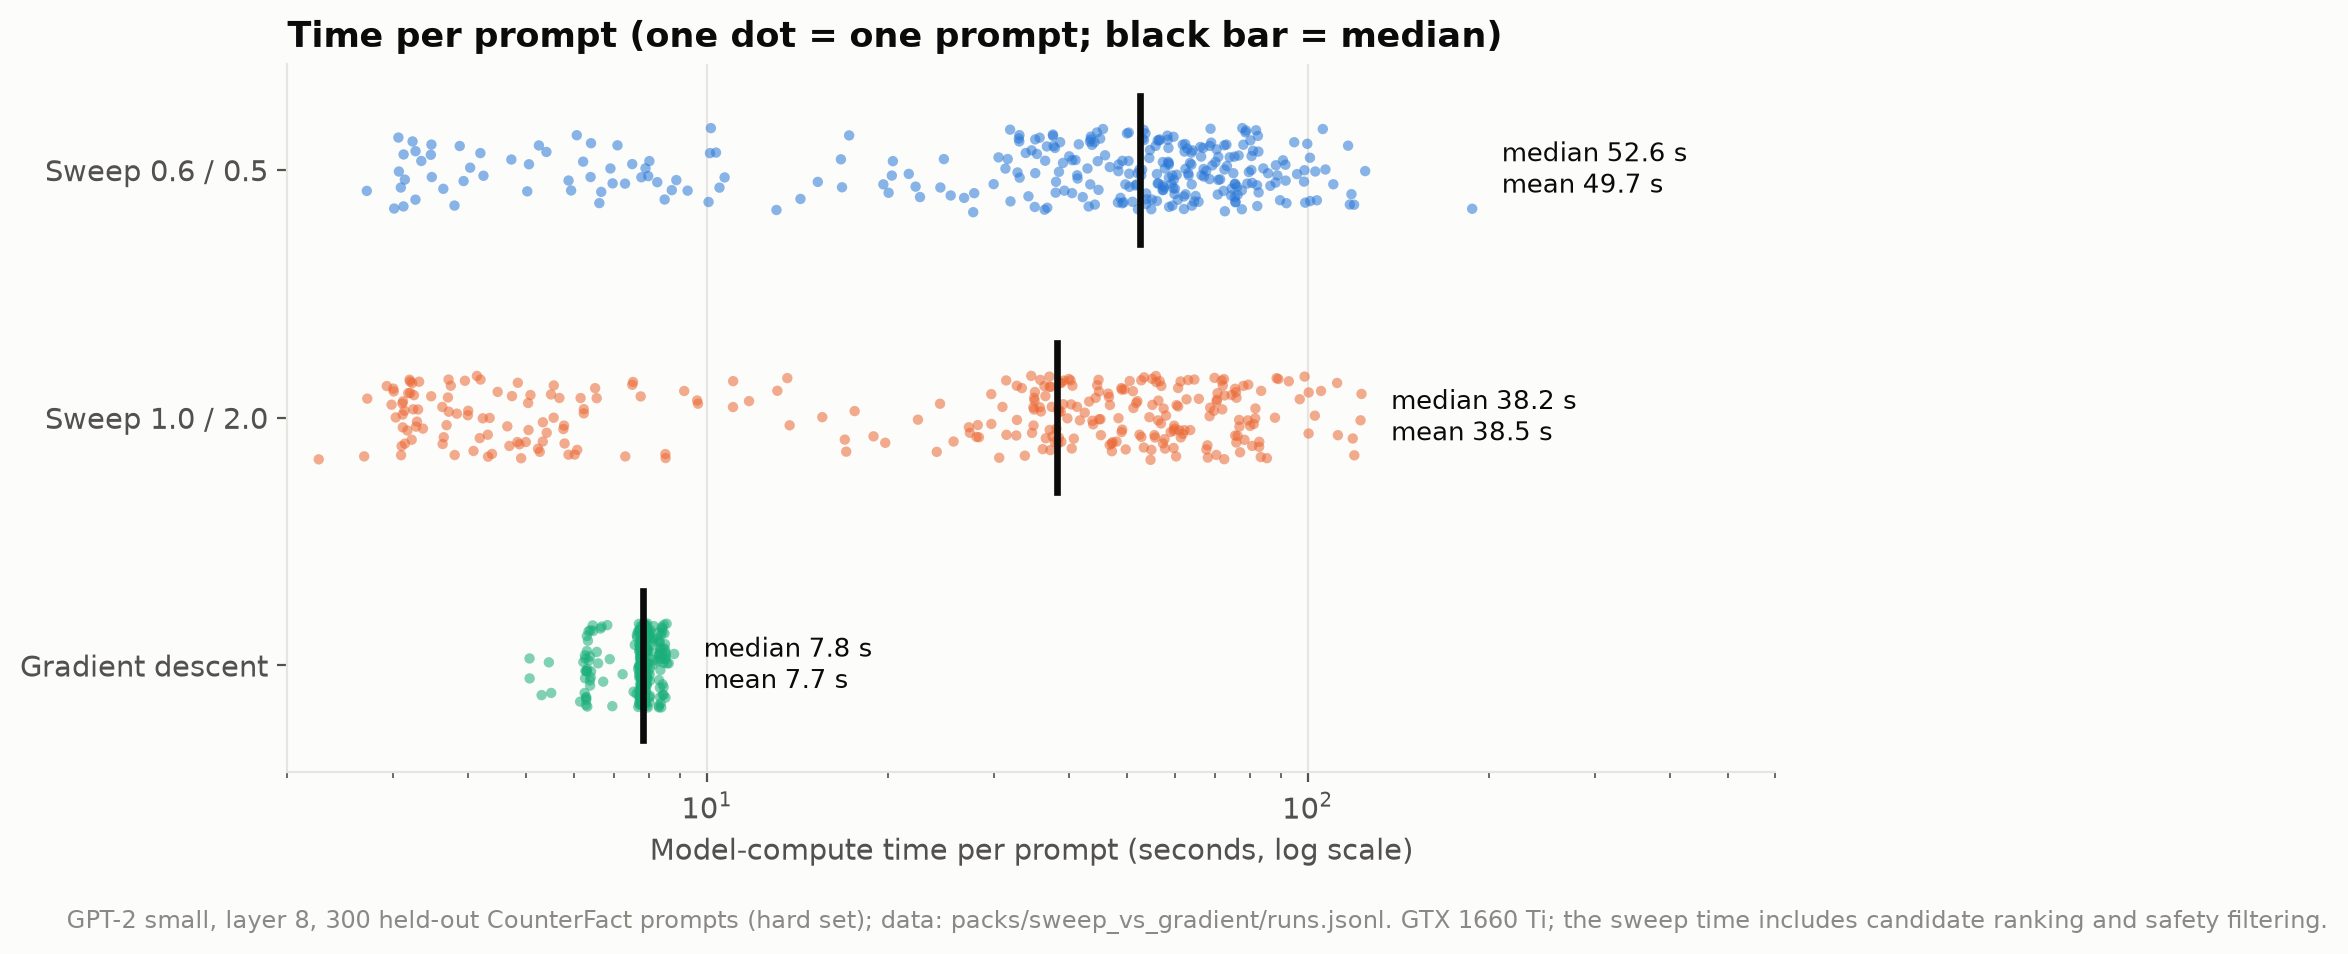
\includegraphics[width=0.85\linewidth]{figures/gd_time}
\caption{Model-Compute Time per Prompt (Log Axis; Black Bar = Median). The Two Clusters of the Sweeps Are the Prompts Solved in a Few Steps and Those Where Several Rounds Ran until the Pool Was Used Up}\label{fig:gd4}
\end{figure}

\textbf{What this shows.} (1) The unequal budget explained a large part of the earlier gap but not all of it: widening the sweep to the same 0 to 3 range took it from 94 to 161 successes, while gradient descent with the same range solved 271, including 110 that the wide sweep did not, and the wide sweep solved none that gradient descent missed. (2) Gradient descent did not produce larger side effects than the sweeps on the prompts that they solved too: its same-prompt KL was lower on 92 of 94 shared successes against the original sweep and on 160 of 161 against the wide sweep (Figure~\ref{fig:gd2}), and its edit was smaller on 148 of 161 against the wide sweep (median 0.13 of the residual norm against 0.32) and about equal against the original sweep (smaller on 57 of 94; medians 0.105 and 0.116). On the 20 unrelated prompts its interference (0.0088) is lower than that of the wide sweep (0.0292) and higher than that of the original sweep (0.0045), which changes less because it succeeds less (Figure~\ref{fig:gd3} plots success against side effects for each band). (3) It is about 5 to 6.5 times faster than the sweeps on the same machine (7.7 s against 38.5 s and 49.7 s of model-compute time, Figure~\ref{fig:gd4}; the sweep time includes its candidate ranking and safety filtering). (4) It is weakest in the hardest band. Of its 271 successes, the median target probability is 7.7\% (79 below 5\%), the KL exceeds 1 on 16 and 2 on none; its 29 failures have a median final rank of 4 and a median KL of 0.94 (largest 2.43).

\textbf{What it does not show.} Part of the KL advantage is by construction: the gradient-descent loss contains a KL term (weight 3.0, switched on once the target leads) and the sweep has none, so a lower KL is partly what the loss was written to do; the comparison is valid as method against method but does not show that gradient descent is naturally gentle. Rank 1 is a low bar: with sampling, targets at a few per cent probability would rarely appear. Only the next word at the last position of the same prompt, plus 20 unrelated prompts, was measured here, so whether the 54 hard-band successes recover anything the model represents or simply write the answer in is not known. Only two sweep configurations were run (the tolerance and graded modes, and the learned pair of Section~\ref{sec:learned}, were not), the two methods optimise different things (the sweep stops at the first success; gradient descent minimises a loss for 100 steps; both know the target), and there is one run, one seed and one machine.

\section{The Additive Edit and Its Controls}\label{sec:additive}

A multiplier cannot switch on a feature that is silent, and the 29 prompts that gradient descent failed on, and the hand trials with implausible targets, are mostly deep targets where the helpful features may be silent. The additive extension of Section~\ref{sec:additive-def} lets the optimiser also add volume to silent features at the last position. Its first hand trials, on six prompts that the multiplier edit had failed (Appendix~B.5), were encouraging: all six reached rank 1 (multipliers alone: one of the six, and that one with a KL of 4.39), with a lower same-prompt KL in five of the six (on ``Aryan'' it rose from 0.32 to 0.58). But the edits were 57\% to 161\% of the residual norm at the last position, whereas free residual pushes of 10 to 20\% of the norm at the last token reached rank 1 on 47 to 99\% of the cached prompts in the headroom study (Section~\ref{sec:headroom}), and every prompt tried in the new tab reached the target, even the most arbitrary ones. That raised the question of whether rank 1 meant anything for this edit.

\textbf{Control with random targets.} Each of 20 validation prompts was paired with a random, unrelated single-token word drawn from the whole vocabulary (starting ranks from about 270 to 44,600, most above 10,000), and the editors were run with 100 steps and $N$ = 200. Multipliers alone reached rank 1 on 1 of the 20 (median edit 39\% of the residual norm); the additive edit reached rank 1 on 20 of 20 at cap factor 1.0 (median edit 192\%) and on 20 of 20 at cap factor 0.25 (126\%) (Figure~\ref{fig:additive}). The additive edit is strong enough to force almost any word to rank 1, with an edit larger than the residual signal itself. It is the analogue of fitting random labels in deep learning, and reaching rank 1 with it is not evidence that anything the model knows was recovered.

\begin{figure}[H]
\centering
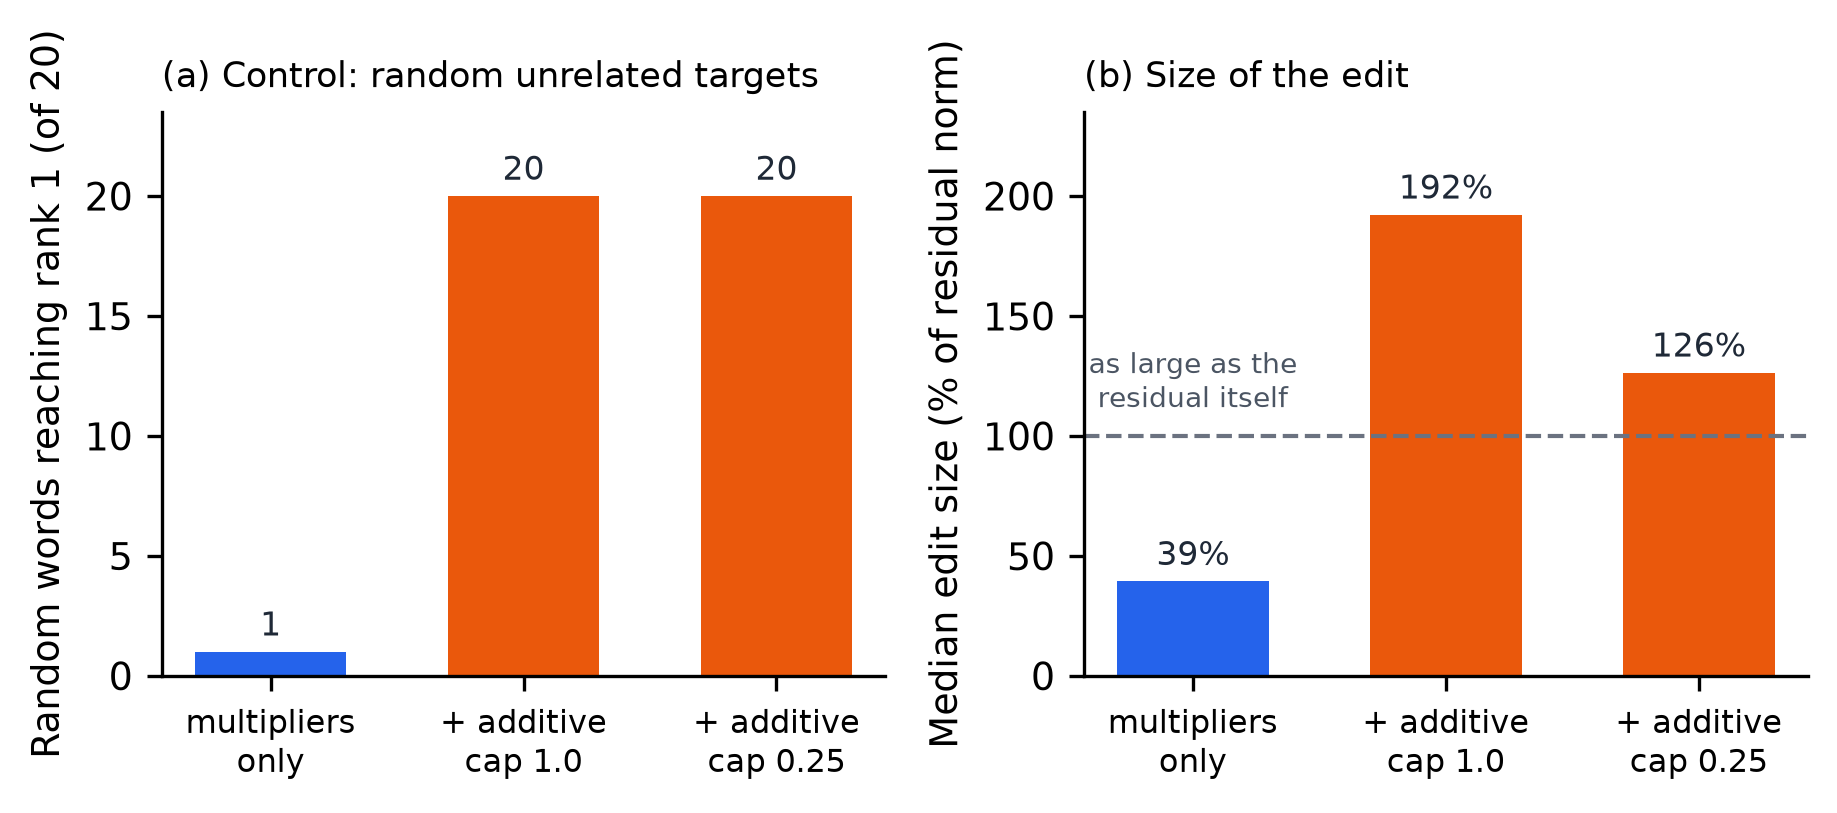
\includegraphics[width=0.88\linewidth]{figures/fig_additive}
\caption{Control with Random Unrelated Targets: (a) Prompts Reaching Rank 1 of 20; (b) Median Size of the Edit as a Share of the Residual Norm}\label{fig:additive}
\end{figure}

\textbf{Reworded and nearby prompts.} An edit tuned on one prompt was applied unchanged, by feature id, to the fact's CounterFact paraphrase prompts (80 in total for 40 test prompts, 10 per band), to up to 10 neighbourhood prompts per fact (other subjects of the same relation; 400 in total) and to the 20 unrelated prompts, once with the true answer as target and once with a random unrelated word (Table~\ref{tab:reworded}, Figure~\ref{fig:reworded}). The additive edit carries over to reworded prompts as well for a random word (median rank 4 against 17,504 unedited, rank 1 on 25\%) as for the true answer (median rank 4.5 against 93.5, rank 1 on 16\%), and the same push moves the top word on 82\% of the unrelated prompts for random targets. The transfer therefore carries no information about the fact: it is a prompt-independent push toward the target word. The multiplier edit behaves differently for the two kinds of target. For true answers the median rank on reworded prompts fell from 93.5 to 36 and 9\% reached rank 1; for random words it fell from 17,504 to 11,832 and none did. This is consistent with a modest fact-related component in the multiplier edit, but it is not a clean test, because the two sets start at very different ranks and ``improved'' counts any improvement however small (96\% for random words, with a mean gain of only 0.19 in $\log_{10}$ rank against 0.30 for true answers). Even for true answers the multiplier edit puts the target at rank 1 on only about one in ten reworded prompts, so an edit tuned on one prompt is mostly local.

\begin{table}[H]
\centering
\caption{Edits Tuned on One Prompt and Applied to Other Prompts (40 Test Prompts, True Answers against Random Words)}\label{tab:reworded}
{\small\renewcommand{\arraystretch}{1.15}
\begin{tabular}{|>{\raggedright\arraybackslash}p{0.266\linewidth}|>{\raggedleft\arraybackslash}p{0.084\linewidth}|>{\raggedleft\arraybackslash}p{0.089\linewidth}|>{\raggedleft\arraybackslash}p{0.089\linewidth}|>{\raggedleft\arraybackslash}p{0.084\linewidth}|>{\raggedleft\arraybackslash}p{0.089\linewidth}|>{\raggedleft\arraybackslash}p{0.089\linewidth}|}
\hline
\textbf{Measure} & \textbf{True: mult. only} & \textbf{True: add 1.0} & \textbf{True: add 0.25} & \textbf{Random: mult. only} & \textbf{Random: add 1.0} & \textbf{Random: add 0.25} \\ \hline
Tuned prompt at rank 1 (of 40) & 36 & 40 & 40 & 1 & 40 & 39 \\ \hline
Median edit size (share of residual norm) & 21\% & 29\% & 23\% & 40\% & 177\% & 119\% \\ \hline
Reworded prompts where the rank improved & 79\% & 88\% & 86\% & 96\% & 100\% & 100\% \\ \hline
Reworded prompts at rank 1 & 9\% & 16\% & 15\% & 0\% & 25\% & 16\% \\ \hline
Median rank on reworded prompts (unedited: 93.5 true, 17,504 random) & 36 & 4.5 & 11.5 & 11,832 & 4 & 9 \\ \hline
Nearby facts: top word changed & 20\% & 32\% & 26\% & 24\% & 72\% & 65\% \\ \hline
20 unrelated prompts: mean KL & 0.010 & 0.229 & 0.108 & 0.016 & 2.273 & 1.518 \\ \hline
20 unrelated prompts: top word changed & 6\% & 24\% & 17\% & 10\% & 82\% & 74\% \\ \hline
\end{tabular}}
\end{table}

\begin{figure}[H]
\centering
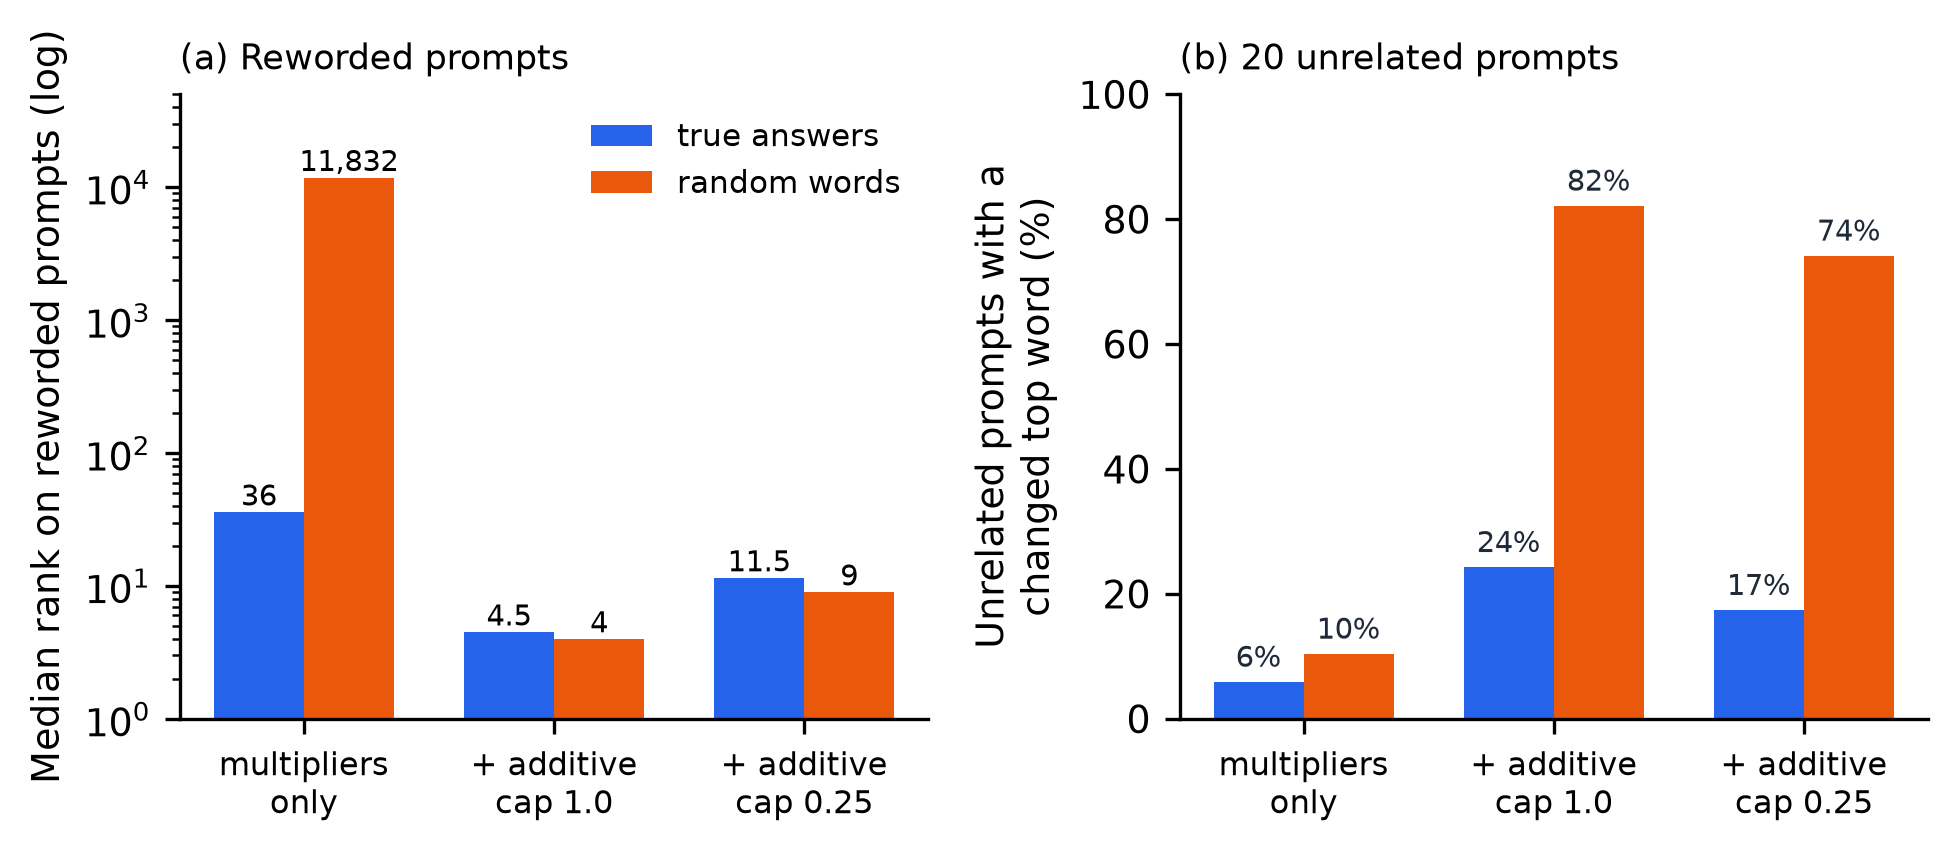
\includegraphics[width=0.95\linewidth]{figures/fig_reworded}
\caption{Transfer of an Edit Tuned on One Prompt: (a) Median Rank of the Target on Reworded Prompts (Unedited: 93.5 for True Answers, 17,504 for Random Words); (b) Share of 20 Unrelated Prompts Whose Top Word Changes}\label{fig:reworded}
\end{figure}

\textbf{A correction.} Earlier notes classified 8 of the 46 ROME facts as ``knowledge absent (unfixable)'', and later notes read deep prompts the same way: if steering could not bring a target near the top, the model did not represent it. That rule does not hold. ``Could not be reached'' described the tool, not the model: multipliers can only rescale features that are already active, whereas the additive edit brought random, unrelated words to rank 1 on 20 of 20 prompts. So failure to steer with a weak tool is not evidence that the model lacks a fact, and success with a strong tool is not evidence that it has one. Reachability by steering cannot serve as the test for whether a model holds a fact, in either direction, and the earlier classification was withdrawn as a statement about the model; it remains only as a choice of evaluation set, as in ROME. The additive edit uses the mechanism of feature injection, adding decoder directions to the residual stream, but in a narrow form: its content is selected by the gradient of the target token's margin, so it writes the answer's output direction and not a representation of a fact, and its amounts do not depend on the prompt, which is why a random word transfers to reworded prompts as well as a true answer does. A graded measure, the size of the smallest additive edit that brings the target to rank 1, compared with controls that start at a matched rank, could replace reachability; it was not run, and the comparison of edit sizes in Table~\ref{tab:reworded} (29\% for true answers against 177\% for random words) is largely circular, because the two sets start at median ranks of 94 and 17,504.

\section{Beyond the Next Word: Generated Text and Instructions}\label{sec:beyond}

The editors are tuned on the next word only, but a model that is edited while it generates keeps reading the edited state. Two questions were tested on the same 40 test prompts (10 per band, true targets): does the edit damage the text that follows, and does it respect an instruction? Each tuned edit was applied to the original prompt, and the model continued for 20 tokens by greedy decoding, with the edit either kept on for the generated tokens or applied to the prompt only; the additive part is added once, at the prompt's last position. Fluency is the perplexity of the continuation under the unedited model. Instruction sensitivity was tested by adding a prefix to the same prompt and applying the same edit: ``Do not say the word X.'' or ``X is the wrong answer.'', with X the target.

\begin{table}[H]
\centering
\caption{Text Quality over 20 Generated Tokens (40 Prompts, True Targets)}\label{tab:genquality}
{\small\renewcommand{\arraystretch}{1.15}
\begin{tabular}{|>{\raggedright\arraybackslash}p{0.254\linewidth}|>{\raggedleft\arraybackslash}p{0.103\linewidth}|>{\raggedleft\arraybackslash}p{0.085\linewidth}|>{\raggedleft\arraybackslash}p{0.122\linewidth}|>{\raggedleft\arraybackslash}p{0.122\linewidth}|>{\raggedleft\arraybackslash}p{0.132\linewidth}|}
\hline
\textbf{Run} & \textbf{Distinct 2-grams} & \textbf{Loops} & \textbf{Target in text} & \textbf{Target repeats} & \textbf{Tail perplexity} \\ \hline
No edit & 0.93 & 0\% & 12\% & 0.03 & 4.7 \\ \hline
Multipliers only, edit kept on & 0.85 & 12\% & 90\% & 0.68 & 4.4 \\ \hline
Multipliers only, prompt only & 0.88 & 8\% & 90\% & 0.65 & 4.2 \\ \hline
Additive cap 1.0, edit kept on & 0.86 & 8\% & 100\% & 0.57 & 4.8 \\ \hline
Additive cap 1.0, prompt only & 0.88 & 2\% & 100\% & 0.65 & 4.7 \\ \hline
Additive cap 0.25, edit kept on & 0.89 & 2\% & 100\% & 0.68 & 4.8 \\ \hline
Additive cap 0.25, prompt only & 0.89 & 2\% & 100\% & 0.70 & 4.3 \\ \hline
\end{tabular}}
\end{table}

\begin{table}[H]
\centering
\caption{Instruction Test: Share of Prompts on which the Target Word Is the Top Choice (40 Prompts)}\label{tab:instruction}
{\small\renewcommand{\arraystretch}{1.15}
\begin{tabular}{|>{\raggedright\arraybackslash}p{0.298\linewidth}|>{\raggedleft\arraybackslash}p{0.119\linewidth}|>{\raggedleft\arraybackslash}p{0.149\linewidth}|>{\raggedleft\arraybackslash}p{0.139\linewidth}|>{\raggedleft\arraybackslash}p{0.139\linewidth}|}
\hline
\textbf{Prompt} & \textbf{No edit} & \textbf{Multipliers only} & \textbf{Additive cap 1.0} & \textbf{Additive cap 0.25} \\ \hline
Plain prompt & 0\% & 90\% & 100\% & 100\% \\ \hline
``Do not say the word X.'' & 45\% & 68\% & 90\% & 88\% \\ \hline
``X is the wrong answer.'' & 30\% & 68\% & 88\% & 85\% \\ \hline
\end{tabular}}
\end{table}

\begin{figure}[H]
\centering
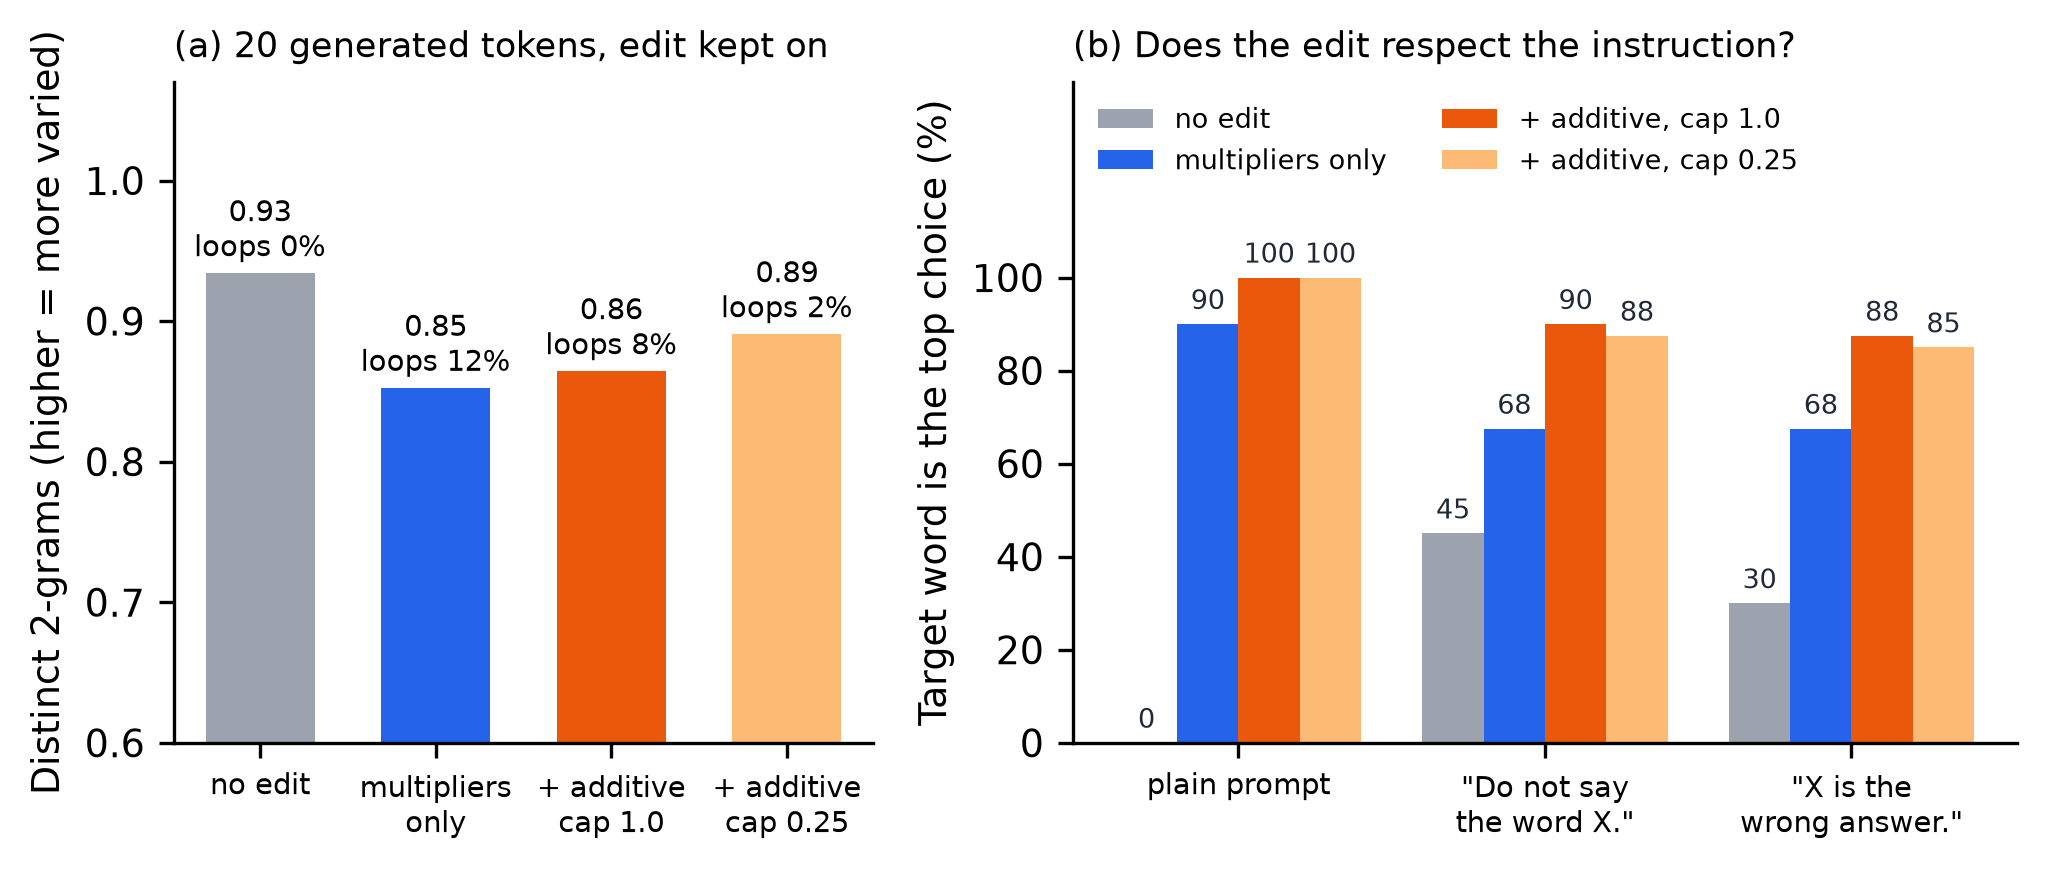
\includegraphics[width=0.98\linewidth]{figures/fig_genquality}
\caption{Generated Text and Instruction Sensitivity: (a) Variety of 20 Generated Tokens with the Edit Kept On; (b) Share of Prompts on which the Target Word Is the Top Choice}\label{fig:genq}
\end{figure}

Table~\ref{tab:genquality} and Figure~\ref{fig:genq}(a) give the text quality. Fluency was unchanged (tail perplexity 4.2 to 4.8 against 4.7 without the edit) and variety fell a little (distinct 2-grams 0.85 to 0.89 against 0.93); loops, a three-word phrase repeated three or more times, appeared in 2\% to 12\% of the continuations against none without the edit, the multiplier edit with the edit kept on being the worst. The target word was repeated far more than without the edit, about 0.6 to 0.7 extra times per continuation. This is a mild effect and not a collapse. At 20 tokens the unedited model does not loop, whereas greedy decoding of GPT-2 Small loops by itself over longer continuations, as was seen in the application, in line with the known behaviour of likelihood-maximising decoding \cite{r35}; the rates above are therefore best read against the unedited model's own repetition under the same decoding rule.

The instruction was largely ignored (Table~\ref{tab:instruction}, Figure~\ref{fig:genq}(b)). Naming the word in the prompt already makes the unedited model put it first in 45\% (``Do not say'') and 30\% (``wrong answer'') of the prompts, because a named word primes copying; with the edit the shares rose to 68\% for the multiplier edit and to 85 to 90\% for the additive edit, and the median rank of the word was 2 without and 1 with the edit in every arm. The edit therefore pushes the word beyond the prompt's own priming and does not respond to what the prompt asks, the additive edit more strongly than the multiplier edit.

A hand check in the application shows the same leak on other prompts. With the additive edit tuned on ``The capital of France is'' $\rightarrow$ `` Hong'' (rank 3419 $\rightarrow$ 1) and kept on, ``The capital of Germany is'' continued with `` Hong Kong, and the city's residents'' instead of `` now home to a new breed of German'' (KL 0.59), and for ``Two plus two is'' the top word stayed `` a'' but its probability fell from 25.0\% to 6.9\% (KL 0.81). This is one prompt each and not a measurement. A control that separates the edit from the ordinary copying of words already present in a prompt that contains the edited text (the unedited model on the same text) has not been run, and neither has the random-target version of this test.

\section{Discussion}\label{sec:discussion}

\textbf{The supply of features limits a multiplicative edit.} Drawing candidates from all prompt positions enlarged the pool about fivefold and raised the number of prompts at rank 1 from 4 to 10 of 13, and every last-token failure ended because the active features had been used up. The strict filter permanently removed few features (2.5 to 2.9\%), because it mostly assigns a feature to the mute side or the boost side, and relaxing it gained at most one prompt whereas removing it lost prompts. These observations are consistent with the number of active features being the principal limit of a multiplicative edit at one layer, but they do not rule out other limits; and scaling cannot activate a feature that is off.

\textbf{What helped most was the choice of features and of strengths, not stronger interventions.} The largest early gains came from muting the drivers of the competitor instead of the helpers of the target, and from combining muting with boosting. Strengthening a single shared feature by 73\% had almost no effect. At the level of strengths, a single better global pair raised the stand-in success rate from 25\% to 39\%, choosing per prompt added nothing measurable, and tuning one multiplier for every feature on the prompt itself did far better (271 of 300 on the real model).

\textbf{Softmax coupling makes the response non-monotonic.} Because edits propagate additively through later layers but pass through a softmax at the output, probability deltas are not additive, a polysemantic boost can help a competitor more than the target, and rank and probability can move in opposite directions. This justifies the per-feature safety filter, the best-step rule, and the choice to report rank together with probability.

\textbf{Depth has a plateau.} Effectiveness rose to layers 6 to 9 and fell toward both ends; layer 8 is a reasonable default and not an established optimum.

\textbf{What the gradient-descent result is.} It is a clear, statistically solid improvement over the hand-built sweep on the measure it was built for, with lower same-prompt side effects, and it is faster. It is not evidence that the model's knowledge was recovered. The median target probability at rank 1 is 7.7\%, the loss contains the side-effect term, and the additive control shows that a strong enough edit reaches rank 1 for any word.

\textbf{What the edit is.} The edit is a push toward the answer's output direction. Its transfer to reworded prompts is real for true answers but small for the multiplier edit, its leak into unrelated prompts is small for the multiplier edit and large for the additive edit, and it largely ignores an instruction that tells the model not to say the word. These are properties of the edit's behaviour. The inference that a target that could not be steered is absent from the model was withdrawn, so no claim is made here, in either direction, about what GPT-2 Small knows. The limits of the evidence are collected in Section~\ref{sec:threats}.

\section{Threats to Validity and What Is Not Shown}\label{sec:threats}

\begin{itemize}
  \item One model (GPT-2 Small), one SAE release (an older 2024 release), and layer 8 in all later studies; nothing here says the findings transfer to other models or layers.
  \item The early studies rely on small, hand-assembled prompt sets (22, 12, 13, 45 and 131 prompts), whose prompts share templates and are not independent draws; the tests treat prompts as independent and are uncorrected for multiple comparisons. The 300-prompt comparison is on held-out CounterFact prompts, which are also templated.
  \item Success is rank 1 on the next token. Its median target probability is only 7.7\% for gradient descent, so it is a low bar; the side-effect measures cover the same prompt, 20 unrelated prompts, and small tests of reworded and nearby prompts and of generated text, not a full CounterFact-style evaluation.
  \item Several results are stand-ins measured on cached states and not on the real system (the headroom and the learned strengths); the real sweep was never run with the learned strengths.
  \item The tests of reworded prompts and of generated text use 40 prompts, one seed and no confidence intervals; the generation and instruction tests were run only with true targets; no control with matched starting ranks was run.
  \item The repair diagnostics concern three prompts chosen because they had failed.
  \item Timings were measured on one machine at a time, with model-compute time that excludes network lookups; they are not comparable across devices.
  \item \textbf{No comparison with ROME, MEMIT, in-context editing, prompting or difference-of-means steering has been run}, so nothing in this report says how the approach ranks against them.
  \item The editing and safety code has no unit-test suite; equivalence between code paths was checked with scripts.
\end{itemize}


% ------------------------------------------------------------
\chapter{Conclusion and Future Work}\label{ch:conclusion-and-future-work}

\section{Conclusion}

This project developed FeatureScalpel, a system for transient, weight-free intervention on sparse autoencoder features in GPT-2 Small, aimed at correct answers that the model ranks below competing tokens. The system classifies prompts by an operational eligibility rule, selects features by measured causal effect and not by activation magnitude, applies reconstruction-error-preserving delta patches to the residual stream, and edits it in a single forward pass in two ways: a Hybrid Mute \& Boost sweep with safety filtering, best-step tracking and pool refill, and per-feature gradient descent. No model weight is modified, and every edit disappears when the forward pass ends. A batch engine, a CounterFact-based benchmark and a set of controls make the results reproducible, and the system runs on NVIDIA GPUs, Apple silicon and CPUs.

The experiments produced five findings. First, for the sweep, the supply of usable features is the limit: drawing candidates from all prompt positions brought the target to rank 1 on 10 of 13 comparable prompts against 4 of 13 for the last token, every last-token failure ended with the active features used up, and the per-feature safety filter was worth keeping, since removing it lost 10 of 29 successes in the pilot while relaxing it added at most one prompt. Second, on 300 held-out CounterFact prompts, per-feature gradient descent reached rank 1 on 271 prompts against 161 for a sweep given the same allowed range and 94 for the original settings, with a lower same-prompt side effect on 160 of the 161 prompts that both solved and about 5 to 6.5 times less compute time; part of the side-effect advantage is by construction of its loss, and its median target probability at rank 1 is only 7.7\%. Third, learned strengths gave a better global default (25.0\% to 38.7\% under a stand-in measure) but no measurable gain from choosing strengths per prompt. Fourth, rank 1 is a weak test: an additive edit that switches on silent features pushed random unrelated words to rank 1 on 20 of 20 prompts and transferred to reworded prompts as well for a random word as for a true answer, so reachability by steering is not evidence about what the model knows, and the early ``knowledge absent'' classification was withdrawn; the multiplier edit shows a small fact-related transfer to reworded prompts, leaks little into unrelated prompts, but, like the additive edit, largely ignores an instruction not to say the target word, and makes the target word and some repetition more frequent in generated text. Fifth, the engineering of the evaluation mattered as much as the method: batching cut the model calls per prompt and layer from 186 to 6 with identical results, and a thread-safety bug that had silently dropped the start-of-text token in the application server was found, fixed and audited.

The results support the claim that a transient SAE-feature edit can raise a suppressed correct answer to the top of the ranking, and that optimising one multiplier per feature does so more often, with lower same-prompt side effects and faster than a hand-built sweep. They do not support a claim that such edits recover knowledge or are specific to a fact, nor that they outperform weight editing, in-context editing or prompting; the comparison with those methods has not been made.

\section{Future Work}

\begin{enumerate}
  \item \textbf{A specificity benchmark} that measures, for every method on the same prompts, whether the target reaches rank 1, whether it transfers to reworded prompts, whether unrelated prompts stay unchanged, whether generated text stays fluent, and whether an explicit instruction is respected, with true targets, random words and random words whose starting rank matches that of the true answers, and with confidence intervals. This is the most important next step, because it supplies the yardstick for everything else.
  \item \textbf{A more specific multiplier edit}, by adding paraphrase prompts, neighbouring prompts and unrelated prompts to the loss of the gradient-descent editor, then repeating the benchmark.
  \item \textbf{An in-context fact vector}: the difference between the layer-8 state of a prompt that states the fact and of the clean prompt, added to the clean run, in the residual space or in feature space, compared with the additive edit on the same benchmark. The run that states the fact in the prompt is also the prompting baseline.
  \item \textbf{A head-to-head comparison with ROME, MEMIT, in-context editing and difference-of-means steering} on the same prompts and measures, using existing implementations such as EasyEdit \cite{r32}, in a separate environment and timed on one machine. This is the test of the project's central claim.
  \item \textbf{Smaller items:} an option to stop the gradient descent early; a control for the follow-up test (the unedited model on the prompt that contains the edited text); sampling or a repetition penalty in the generation view; multi-token targets; re-selecting the blocker within a round of the sweep; the learned strengths in the real sweep and a full run of FeatureNet; the graded measure of the smallest additive edit; and the all-positions version of the 131-prompt filter study.
  \item \textbf{Other models and attribution:} larger models with pretrained SAEs such as Gemma Scope \cite{r19}, once the pipeline is validated on GPT-2 Small, and faster causal ranking with attribution patching \cite{r16} if the fact sets grow beyond what batched ablation handles.
\end{enumerate}

% ======================= REFERENCES =======================
\clearpage
\phantomsection\addcontentsline{toc}{chapter}{References}
\renewcommand{\bibname}{References}
\begin{thebibliography}{99}
\bibitem{r1} A. Radford, J. Wu, R. Child, D. Luan, D. Amodei, and I. Sutskever, ``Language models are unsupervised multitask learners,'' \textit{OpenAI Technical Report}, 2019.

\bibitem{r2} K. Meng, D. Bau, A. Andonian, and Y. Belinkov, ``Locating and editing factual associations in GPT,'' in \textit{Advances in Neural Information Processing Systems (NeurIPS)}, vol. 35, 2022, pp. 17359--17372.

\bibitem{r3} K. Meng, A. S. Sharma, A. Andonian, Y. Belinkov, and D. Bau, ``Mass-editing memory in a transformer,'' in \textit{Proc. International Conference on Learning Representations (ICLR)}, 2023.

\bibitem{r4} A. Gupta, A. Rao, and G. Anumanchipalli, ``Model editing at scale leads to gradual and catastrophic forgetting,'' in \textit{Findings of the Association for Computational Linguistics: ACL 2024}, 2024; arXiv:2401.07453.

\bibitem{r5} N. Elhage, T. Hume, C. Olsson, \textit{et al.}, ``Toy models of superposition,'' \textit{Transformer Circuits Thread}, 2022.

\bibitem{r6} T. Bricken, A. Templeton, J. Batson, \textit{et al.}, ``Towards monosemanticity: Decomposing language models with dictionary learning,'' \textit{Transformer Circuits Thread}, 2023.

\bibitem{r7} H. Cunningham, A. Ewart, L. Riggs, R. Huben, and L. Sharkey, ``Sparse autoencoders find highly interpretable features in language models,'' in \textit{Proc. International Conference on Learning Representations (ICLR)}, 2024.

\bibitem{r8} A. Templeton, T. Conerly, \textit{et al.}, ``Scaling monosemanticity: Extracting interpretable features from Claude 3 Sonnet,'' \textit{Transformer Circuits Thread}, 2024.

\bibitem{r9} A. M. Turner, L. Thiergart, G. Leech, D. Udell, J. J. Vazquez, U. Mini, and M. MacDiarmid, ``Steering language models with activation engineering,'' \textit{arXiv preprint arXiv:2308.10248}, 2023.

\bibitem{r10} N. Rimsky, N. Gabrieli, J. Schulz, M. Tong, E. Hubinger, and A. M. Turner, ``Steering Llama 2 via contrastive activation addition,'' in \textit{Proc. 62nd Annual Meeting of the Association for Computational Linguistics (ACL)}, 2024, pp. 15504--15522.

\bibitem{r11} A. Zou, L. Phan, S. Chen, \textit{et al.}, ``Representation engineering: A top-down approach to AI transparency,'' \textit{arXiv preprint arXiv:2310.01405}, 2023.

\bibitem{r12} Z. Wu, A. Arora, A. Geiger, Z. Wang, J. Huang, D. Jurafsky, C. D. Manning, and C. Potts, ``AxBench: Steering LLMs? Even simple baselines outperform sparse autoencoders,'' in \textit{Proc. International Conference on Machine Learning (ICML)}, 2025; arXiv:2501.17148.

\bibitem{r13} N. Nanda and J. Bloom, ``TransformerLens,'' GitHub repository, 2022. [Online]. Available: \url{https://github.com/TransformerLensOrg/TransformerLens}

\bibitem{r14} J. Bloom, C. Tigges, A. Duong, and D. Chanin, ``SAELens,'' GitHub repository, 2024. [Online]. Available: \url{https://github.com/decoderesearch/SAELens}

\bibitem{r15} J. Bloom, ``Open source sparse autoencoders for all residual stream layers of GPT2 small,'' \textit{AI Alignment Forum}, 2024.

\bibitem{r16} J. Kram\'ar, T. Lieberum, R. Shah, and N. Nanda, ``AtP*: An efficient and scalable method for localizing LLM behaviour to components,'' \textit{arXiv preprint arXiv:2403.00745}, 2024.

\bibitem{r17} A. Conmy, A. N. Mavor-Parker, A. Lynch, S. Heimersheim, and A. Garriga-Alonso, ``Towards automated circuit discovery for mechanistic interpretability,'' in \textit{Advances in Neural Information Processing Systems (NeurIPS)}, vol. 36, 2023.

\bibitem{r18} A. Syed, C. Rager, and A. Conmy, ``Attribution patching outperforms automated circuit discovery,'' \textit{arXiv preprint arXiv:2310.10348}, 2023.

\bibitem{r19} T. Lieberum, S. Rajamanoharan, A. Conmy, \textit{et al.}, ``Gemma Scope: Open sparse autoencoders everywhere all at once on Gemma 2,'' \textit{arXiv preprint arXiv:2408.05147}, 2024.

\bibitem{r20} J. Lin and J. Bloom, ``Neuronpedia: Interactive reference and tooling for analyzing neural networks,'' 2023. [Online]. Available: \url{https://www.neuronpedia.org}

\bibitem{r21} S. Heimersheim and N. Nanda, ``How to use and interpret activation patching,'' \textit{arXiv preprint arXiv:2404.15255}, 2024.

\bibitem{r22} A. Paszke, S. Gross, F. Massa, \textit{et al.}, ``PyTorch: An imperative style, high-performance deep learning library,'' in \textit{Advances in Neural Information Processing Systems (NeurIPS)}, vol. 32, 2019, pp. 8024--8035.

\bibitem{r23} D. Arad, A. Mueller, and Y. Belinkov, ``SAEs are good for steering -- if you select the right features,'' in \textit{Proc. Conference on Empirical Methods in Natural Language Processing (EMNLP)}, 2025; arXiv:2505.20063.

\bibitem{r24} L. Smith, S. Rajamanoharan, A. Conmy, C. McDougall, T. Lieberum, J. Kram\'ar, R. Shah, and N. Nanda, ``Negative results for SAEs on downstream tasks and deprioritising SAE research (GDM mech interp team progress update \#2),'' \textit{LessWrong}, Mar. 2025. [Online]. Available: \url{https://www.lesswrong.com/posts/4uXCAJNuPKtKBsi28/negative-results-for-saes-on-downstream-tasks}

\bibitem{r25} M. Chaudhary and A. Geiger, ``Evaluating open-source sparse autoencoders on disentangling factual knowledge in GPT-2 small,'' \textit{arXiv preprint arXiv:2409.04478}, 2024.

\bibitem{r26} M. Cui, L. Shen, and X. Yang, ``SAE interventions are unreliable: Post-intervention recovery of suppressed behavior,'' \textit{arXiv preprint arXiv:2606.18322}, 2026.

\bibitem{r27} E. Farrell, Y.-T. Lau, and A. Conmy, ``Applying sparse autoencoders to unlearn knowledge in language models,'' \textit{arXiv preprint arXiv:2410.19278}, 2024.

\bibitem{r28} S. Chalnev, M. Siu, and A. Conmy, ``Improving steering vectors by targeting sparse autoencoder features,'' \textit{arXiv preprint arXiv:2411.02193}, 2024.

\bibitem{r29} Y. Zhao, A. Devoto, G. Hong, X. Du, A. P. Gema, H. Wang, X. He, K.-F. Wong, and P. Minervini, ``Steering knowledge selection behaviours in LLMs via SAE-based representation engineering,'' in \textit{Proc. NAACL}, 2025; arXiv:2410.15999.

\bibitem{r30} P. Hase, M. Bansal, B. Kim, and A. Ghandeharioun, ``Does localization inform editing? Surprising differences in causality-based localization vs.\ knowledge editing in language models,'' in \textit{Advances in Neural Information Processing Systems (NeurIPS)}, vol. 36, 2023.

\bibitem{r31} C. Zheng, L. Li, Q. Dong, Y. Fan, Z. Wu, J. Xu, and B. Chang, ``Can we edit factual knowledge by in-context learning?'' in \textit{Proc. Conference on Empirical Methods in Natural Language Processing (EMNLP)}, 2023; arXiv:2305.12740.

\bibitem{r32} P. Wang, N. Zhang, B. Tian, \textit{et al.}, ``EasyEdit: An easy-to-use knowledge editing framework for large language models,'' in \textit{Proc. 62nd Annual Meeting of the Association for Computational Linguistics (System Demonstrations)}, 2024; arXiv:2308.07269.

\bibitem{r33} S. Marks, C. Rager, E. J. Michaud, Y. Belinkov, D. Bau, and A. Mueller, ``Sparse feature circuits: Discovering and editing interpretable causal graphs in language models,'' in \textit{Proc. International Conference on Learning Representations (ICLR)}, 2025; arXiv:2403.19647.

\bibitem{r34} P. Lewis, E. Perez, A. Piktus, \textit{et al.}, ``Retrieval-augmented generation for knowledge-intensive NLP tasks,'' in \textit{Advances in Neural Information Processing Systems (NeurIPS)}, vol. 33, 2020.

\bibitem{r35} A. Holtzman, J. Buys, L. Du, M. Forbes, and Y. Choi, ``The curious case of neural text degeneration,'' in \textit{Proc. International Conference on Learning Representations (ICLR)}, 2020.

\bibitem{r36} D. P. Kingma and J. Ba, ``Adam: A method for stochastic optimization,'' in \textit{Proc. International Conference on Learning Representations (ICLR)}, 2015.

\bibitem{r37} nostalgebraist, ``Interpreting GPT: the logit lens,'' \textit{LessWrong}, Aug. 2020. [Online]. Available: \url{https://www.lesswrong.com/posts/AcKRB8wDpdaN6v6ru/interpreting-gpt-the-logit-lens}

\bibitem{r38} M. Geva, R. Schuster, J. Berant, and O. Levy, ``Transformer feed-forward layers are key-value memories,'' in \textit{Proc. Conference on Empirical Methods in Natural Language Processing (EMNLP)}, 2021.

\bibitem{r39} Q. McNemar, ``Note on the sampling error of the difference between correlated proportions or percentages,'' \textit{Psychometrika}, vol. 12, no. 2, pp. 153--157, 1947.

\bibitem{r40} F. Wilcoxon, ``Individual comparisons by ranking methods,'' \textit{Biometrics Bulletin}, vol. 1, no. 6, pp. 80--83, 1945.
\end{thebibliography}


% ======================= APPENDICES =======================
\clearpage
\chapter*{Appendices}
\addcontentsline{toc}{chapter}{Appendices}
\setcounter{figure}{0}\renewcommand{\thefigure}{A.\arabic{figure}}\renewcommand{\theHfigure}{A.\arabic{figure}}
\section*{Appendix A: User Interface Layouts}
\addcontentsline{toc}{section}{Appendix A: User Interface Layouts}
Figures~\ref{fig:ui_hybrid} and~\ref{fig:ui_proto} show the layout of the two tabs of the final application (\texttt{experiment\_\allowbreak{}app.\allowbreak{}py}) that carry the editing methods, redrawn as schematics from the code. The other five tabs (Monosemanticity Analysis, Session history and benchmarks, Sequential vs Batched Proof, Batch: Last vs All Tokens, and Repair \& SAE limit) are described in Chapter~\ref{ch:implementation}. Figures~\ref{fig:ui_app} and~\ref{fig:ui_bench} show the two early applications of the first stage of the project. Screenshots of the running applications can be placed alongside the schematics.

\begin{figure}[H]
\centering
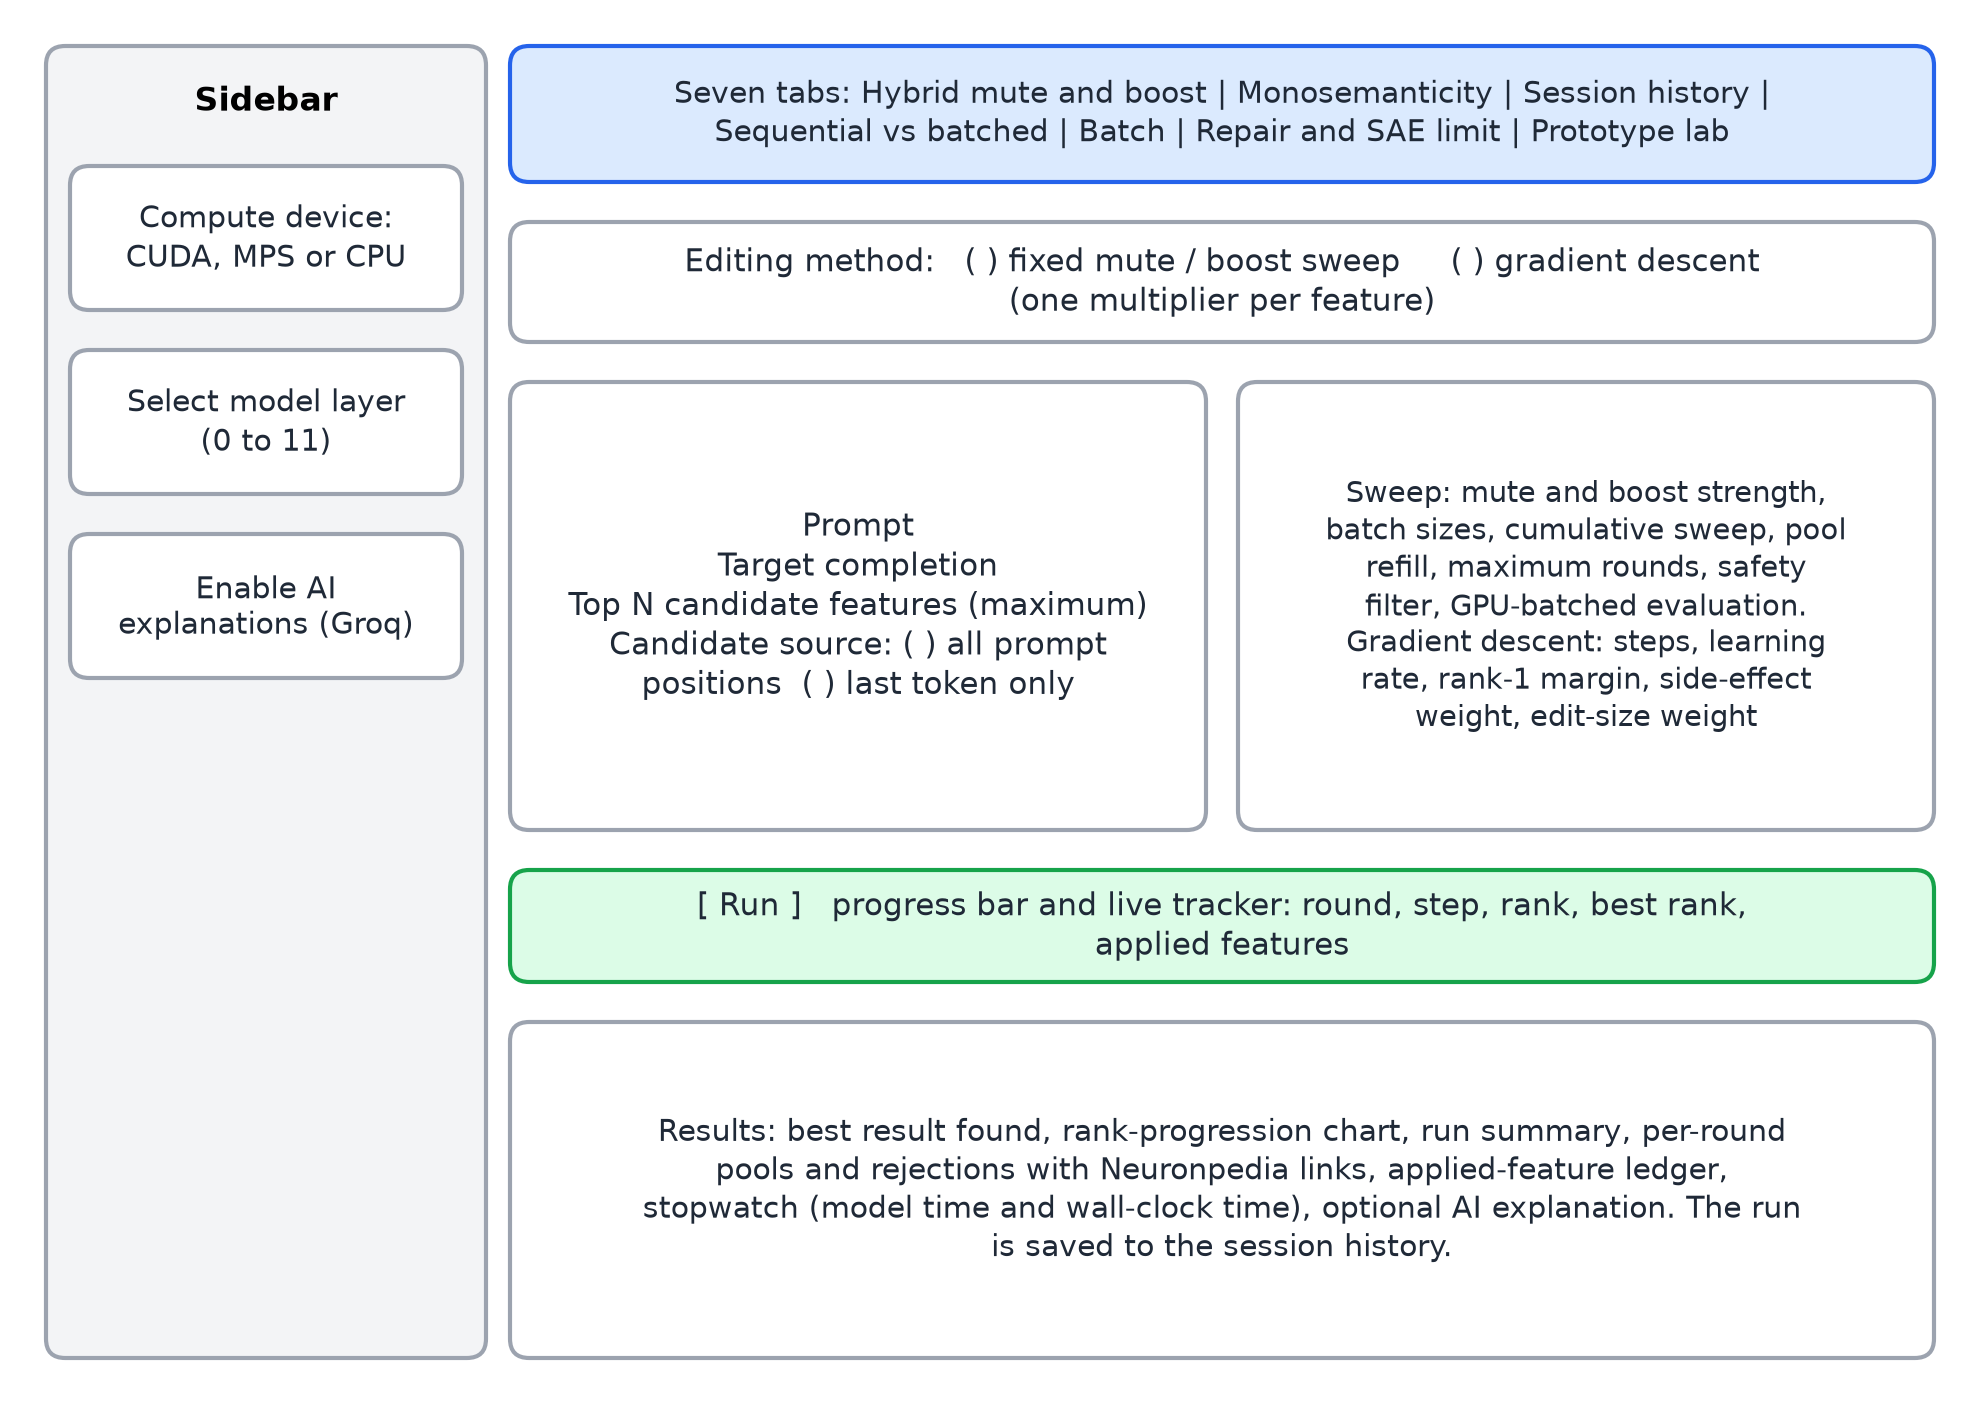
\includegraphics[width=0.92\linewidth]{figures/fig_ui_hybrid}
\caption{Layout of the Hybrid Mute and Boost Tab of the Final Application (experiment\_app.py), with the Choice between the Fixed Sweep and Gradient Descent}\label{fig:ui_hybrid}
\end{figure}

\begin{figure}[H]
\centering
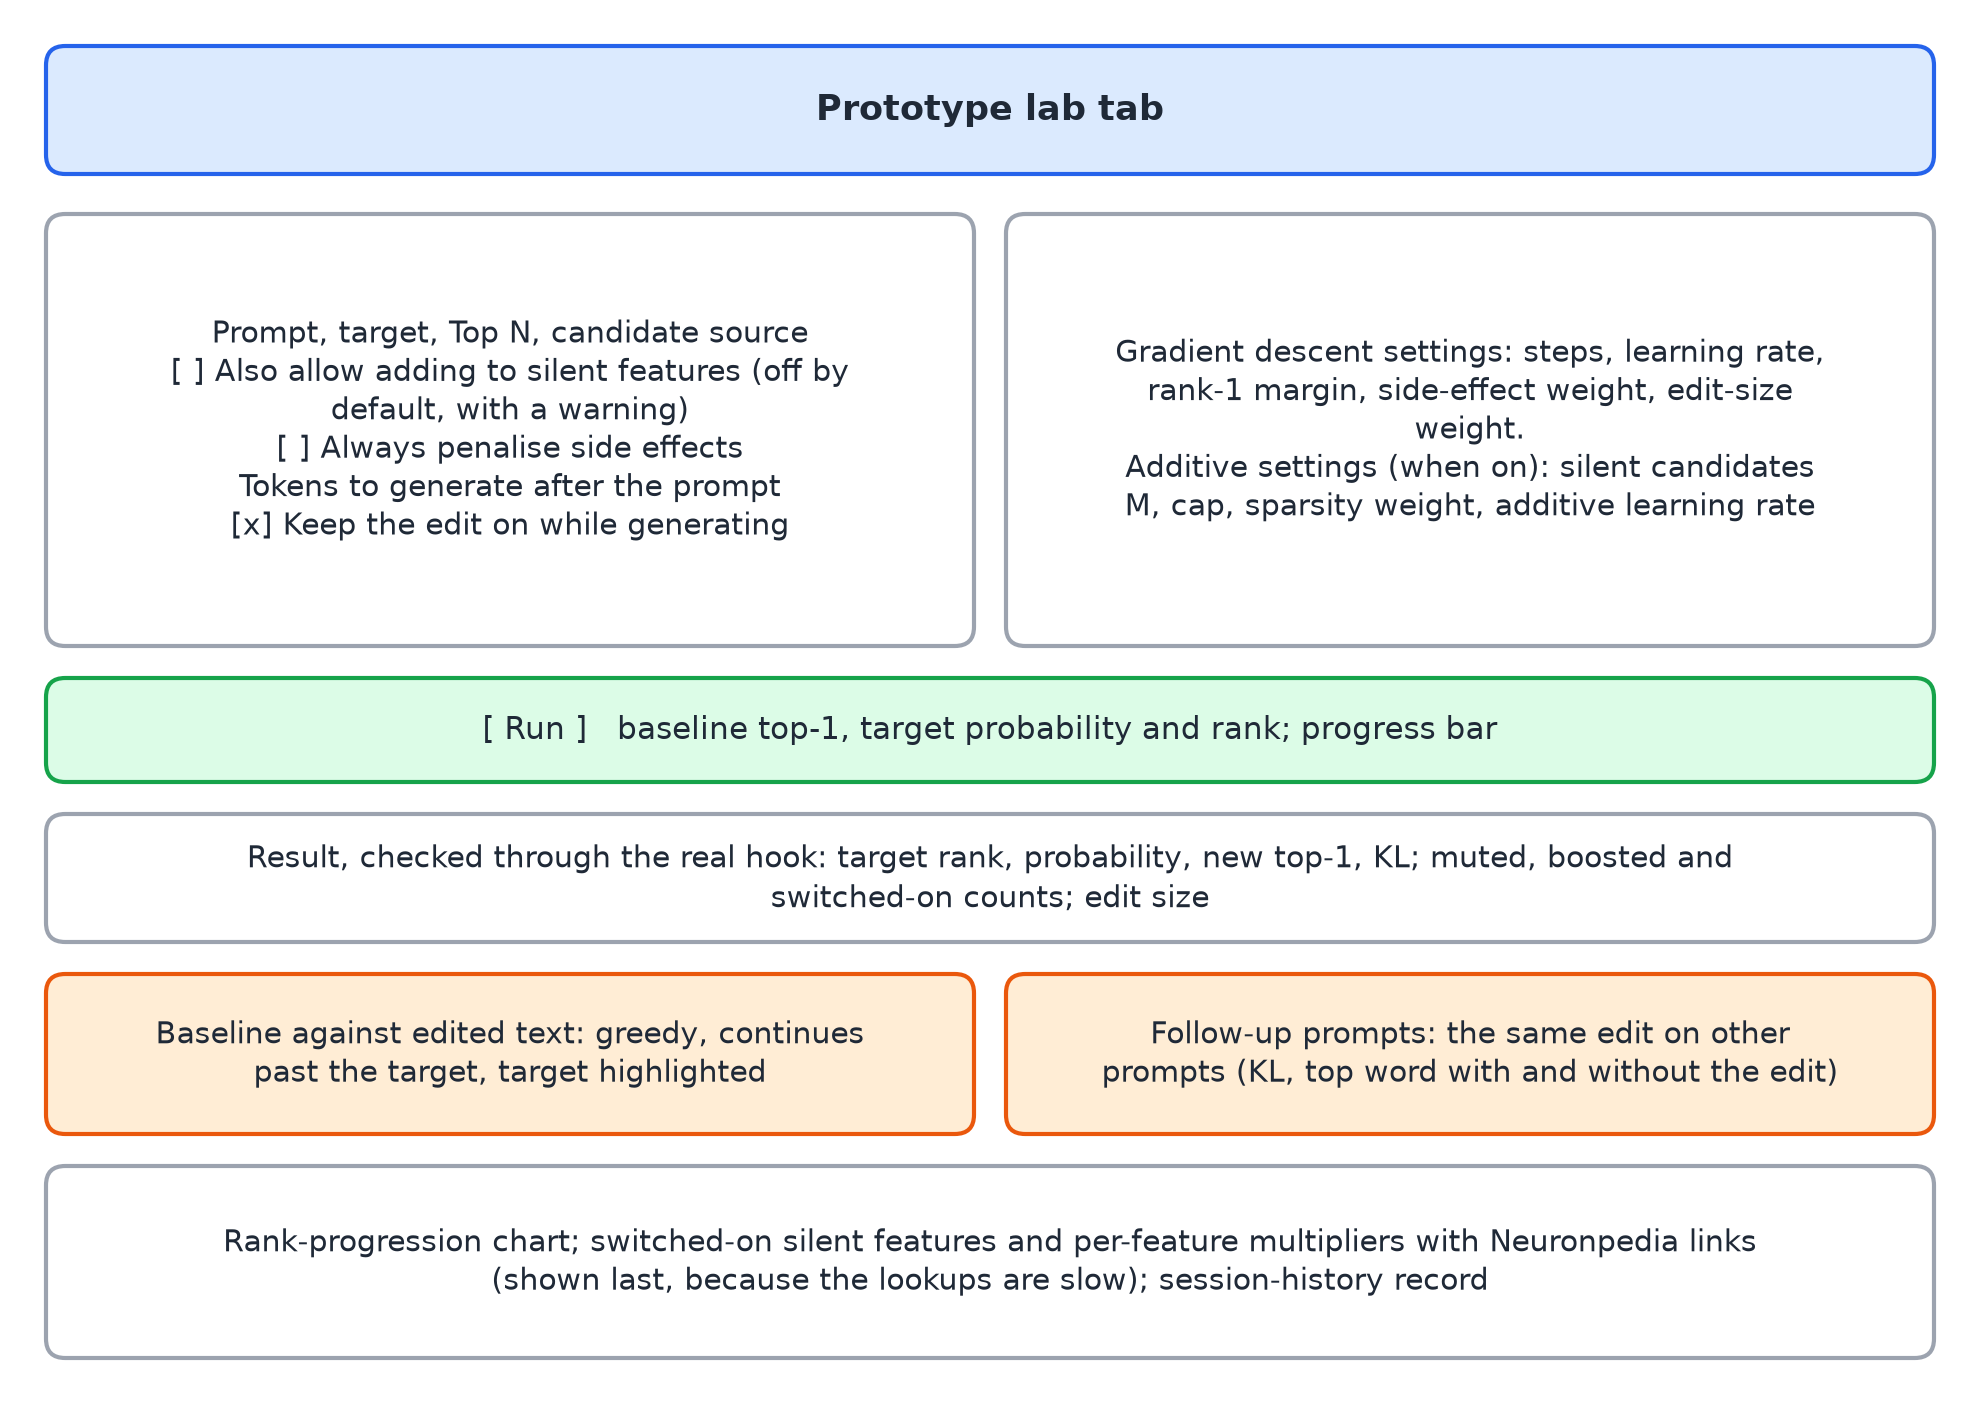
\includegraphics[width=0.92\linewidth]{figures/fig_ui_proto}
\caption{Layout of the Prototype Lab Tab (Gradient-Descent Editor, Optional Additive Edit, Baseline-against-Edited Generation and Follow-Up Prompts)}\label{fig:ui_proto}
\end{figure}

\begin{figure}[H]
\centering
\includegraphics[width=0.92\linewidth]{figures/ui_app}
\caption{Layout of the Causal Feature Steering Application (app.py), an Early Application of the First Stage}\label{fig:ui_app}
\end{figure}

\begin{figure}[H]
\centering
\includegraphics[width=0.92\linewidth]{figures/ui_bench}
\caption{Layout of the Layer Intervention Benchmark Application (layer\_benchmark.py), an Early Application of the First Stage}\label{fig:ui_bench}
\end{figure}

\section*{Appendix B: Additional Technical Details}
\addcontentsline{toc}{section}{Appendix B: Additional Technical Details}
\setcounter{table}{0}\renewcommand{\thetable}{B.\arabic{table}}\renewcommand{\theHtable}{B.\arabic{table}}
\setcounter{figure}{0}\renewcommand{\thefigure}{B.\arabic{figure}}\renewcommand{\theHfigure}{B.\arabic{figure}}
\subsection*{B.1 Benchmark Artifact Schema}
\addcontentsline{toc}{subsection}{B.1 Benchmark Artifact Schema}
Each sweep writes one JSON artifact to the \texttt{benchmark\_\allowbreak{}results/\allowbreak } folder, named with the sweep timestamp. The metadata block records the fields below; each per-layer result records clean and final rank and probability, rank improvement, probability gain, success flag, selected mute and boost feature IDs, top prediction after intervention, stage timings and forward-pass counts.

\begin{lstlisting}[title={Listing B.1: Artifact metadata (abridged)}]
{
  "benchmark_name": "layer_intervention_benchmark",
  "benchmark_version": "0.3",
  "timestamp": "<ISO-8601>",
  "model": "gpt2",
  "sae_release": "gpt2-small-res-jb",
  "hook_location": "hook_resid_pre",
  "safety_enabled": true,
  "selected_layers": [2, 5, 8, 10],
  "parameters": { "mute_strength": 0.3, "boost_strength": 0.5,
                  "mute_batch_size": 3, "boost_batch_size": 3,
                  "use_safety": true, "algorithm": "hybrid_mute_boost" }
}
\end{lstlisting}

\subsection*{B.2 Pretrained SAE Availability}
\addcontentsline{toc}{subsection}{B.2 Pretrained SAE Availability}
An audit of the SAELens registry confirmed that \texttt{gpt2-small-res-jb} contains exactly twelve dictionaries, one at \texttt{blocks.\allowbreak{}L.\allowbreak{}hook\_\allowbreak{}resid\_\allowbreak{}pre} for each L from 0 to 11, and none at other hook points. Dictionaries for other hook points are provided by separate releases: \texttt{gpt2-small-resid-post-jb}, \texttt{gpt2-small-mlp-out-jb}, \texttt{gpt2-small-attn-out-jb} and \texttt{gpt2-small-hook-z-jb}.

\subsection*{B.3 Per-Fact Results of Competitor Ablation}
\addcontentsline{toc}{subsection}{B.3 Per-Fact Results of Competitor Ablation}

{\small\renewcommand{\arraystretch}{1.15}
\begin{longtable}{|>{\raggedright\arraybackslash}p{0.347\linewidth}|>{\raggedright\arraybackslash}p{0.116\linewidth}|>{\raggedright\arraybackslash}p{0.129\linewidth}|>{\raggedright\arraybackslash}p{0.129\linewidth}|>{\raggedright\arraybackslash}p{0.080\linewidth}|}
\caption{Competitor Ablation Results on the 22 Suppressed Facts (strength 0.3, $\leq$ 5 rounds)}\label{tab:competitor-ablation-results-on-the-22-suppressed-facts-strength-0-3-5-rounds}\\
\hline
\textbf{Prompt} & \textbf{Target} & \textbf{Clean prob. / rank} & \textbf{Final prob. / rank} & \textbf{Success} \\ \hline
\endfirsthead
\hline
\textbf{Prompt} & \textbf{Target} & \textbf{Clean prob. / rank} & \textbf{Final prob. / rank} & \textbf{Success} \\ \hline
\endhead
Eavan Boland was born in & Dublin & 1.85\% / 4 & 1.81\% / 3 & No \\ \hline
Knud, Hereditary Prince of Denmark passed away in & Copenhagen & 0.50\% / 45 & 0.45\% / 47 & No \\ \hline
The location of Massachusetts Institute of Technology is in & Cambridge & 1.15\% / 8 & 0.73\% / 11 & No \\ \hline
The location of Galatasaray University is in the heart of & Istanbul & 14.07\% / 2 & 15.84\% / 2 & No \\ \hline
John Pym died in the city of & London & 0.87\% / 10 & 0.68\% / 11 & No \\ \hline
Emilia Rydberg was born in & Stockholm & 0.70\% / 16 & 0.73\% / 14 & No \\ \hline
Joseph Goebbels worked in the city of & Berlin & 4.82\% / 2 & 5.45\% / 2 & No \\ \hline
Francesco Castellacci was born in & Rome & 5.41\% / 2 & 5.31\% / 1 & Yes \\ \hline
2005 Australian Open is located in & Melbourne & 10.27\% / 2 & 9.58\% / 3 & No \\ \hline
Giulio Romano originates from the city of & Rome & 2.52\% / 2 & 2.93\% / 1 & Yes \\ \hline
Euromoney Institutional Investor's headquarters are in & London & 0.99\% / 7 & 1.18\% / 6 & No \\ \hline
Coco Chanel passed away in & Paris & 3.43\% / 2 & 3.85\% / 1 & Yes \\ \hline
The headquarter of Zillow is in downtown & Seattle & 4.12\% / 8 & 3.99\% / 5 & No \\ \hline
Jan Swammerdam died in the city of & Amsterdam & 1.16\% / 9 & 0.90\% / 14 & No \\ \hline
Seiyu Group's headquarters are in & Tokyo & 10.00\% / 2 & 10.95\% / 2 & No \\ \hline
Second French Empire's capital city is & Paris & 1.21\% / 14 & 1.52\% / 12 & No \\ \hline
Henry Somerset, 7th Duke of Beaufort worked in the city of & London & 2.20\% / 2 & 1.51\% / 5 & No \\ \hline
York University can be found in the heart of & Toronto & 7.12\% / 3 & 6.92\% / 3 & No \\ \hline
Rudolf Steiner worked in the city of & Berlin & 2.28\% / 5 & 2.47\% / 5 & No \\ \hline
James Northcote died in the city of & London & 1.38\% / 3 & 1.36\% / 4 & No \\ \hline
2002 Australian Open is located in & Melbourne & 9.42\% / 2 & 8.80\% / 3 & No \\ \hline
Fantastic Fest can be found in the heart of downtown & Austin & 4.41\% / 3 & 3.64\% / 2 & No \\ \hline
\end{longtable}}

\subsection*{B.4 Hand Trials of Gradient Descent and the Fixed Sweep}
\addcontentsline{toc}{subsection}{B.4 Hand Trials of Gradient Descent and the Fixed Sweep}
The first comparison of gradient descent with the sweep was made by hand in the Hybrid tab, on nine prompts chosen by the authors, with one run per setting on the GTX 1660 Ti (Table~\ref{tab:handtrials}, Figure~\ref{fig:gdtrials}). These trials led to the controlled comparison of Section~\ref{sec:gdvs} but are not results themselves: the prompts were hand-picked, the strengths of the sweep differed between rows, gradient descent could scale a feature anywhere from 0 to 3 times whereas the sweep at the strengths used reached only about 0.4 to 1.8 times, and no side effect was measured for the sweep. The runs of gradient descent and the two sweeps on ``powder'' and the one on ``falling'' are in the stored session file; the sweep results marked with an asterisk were read from screenshots and are approximate. Times are the model-compute time of the application, which excludes the Neuronpedia lookups.

\begin{table}[H]
\centering
\caption{Hand Trials of the Fixed Sweep and Gradient Descent (Hybrid Tab, Top N = 200; Exploratory)}\label{tab:handtrials}
{\small\renewcommand{\arraystretch}{1.15}
\begin{tabular}{|>{\raggedright\arraybackslash}p{0.197\linewidth}|>{\raggedleft\arraybackslash}p{0.066\linewidth}|>{\raggedright\arraybackslash}p{0.248\linewidth}|>{\raggedright\arraybackslash}p{0.248\linewidth}|>{\raggedright\arraybackslash}p{0.087\linewidth}|}
\hline
\textbf{Prompt $\rightarrow$ target} & \textbf{Start rank} & \textbf{Fixed sweep (mute / boost)} & \textbf{Gradient descent (steps, side-effect weight, other changes)} & \textbf{Same-prompt KL of gradient descent} \\ \hline
The sky is $\rightarrow$ falling & 2 & \#1 in 6 steps, 4.5 s (0.3 / 0.5) & not run & -- \\ \hline
The sky is $\rightarrow$ powder & 2554 & \#1133 (0.3 / 0.5; 3 rounds, 50 steps, 23.6 s; pool ran out); \#569 (0.6 / 0.8; 49 steps, 21.1 s) & \#179 (100 steps, 3.0; 6.2 s); \#164 (learning rate 0.14, 100, 3.0); \#157 (0.14, 200, 4.0; 12.1 s) & 0.84 / 0.88 / 0.87 \\ \hline
The sky is $\rightarrow$ black & 10 & \#3 (0.6 / 0.8; 53 steps, pool ran out)* & \textbf{\#1} (100, 3.0; 6.2 s) & 0.34 \\ \hline
Frankie Lee Sims died at $\rightarrow$ Dallas & 548 & \#16 (0.6 / 0.7; 3 rounds, 127 steps)* & \textbf{\#1} (100, 3.0; 6.4 s) & 1.88 \\ \hline
Kak\'a professionally plays the sport $\rightarrow$ soccer & 436 & \#101 (0.5 / 0.7; 4 rounds, 174 steps)* & \textbf{\#1} (110, 3.0; 7.0 s) & 1.23 \\ \hline
My nephew is a $\rightarrow$ rapist & 1740 & \#457 (strengths not visible; 3 rounds, 83 steps)* & \#17 (100, 3.0; 6.4 s) & 0.56 \\ \hline
The sky is $\rightarrow$ Adi & 14149 & \#8097 (0.3 / 0.5)* & \#4897 (100, 3.0; 5.9 s) & 2.71 \\ \hline
Hello, my name is $\rightarrow$ Aryan & 13576 & not run & \#2664 (100, 3.0; 6.7 s); \#2284 (learning rate 0.11, 150; 9.6 s) & 0.32 / 0.35 \\ \hline
Hello, my name is $\rightarrow$ Rajesh & 20214 & not run & \#6934 (learning rate 0.15, 300 steps, weight 3.5, margin 0.4; 18.7 s) & 0.25 \\ \hline
\end{tabular}}
\end{table}

Gradient descent ended nearer to rank 1 than the sweep on all six prompts where both were run, and reached rank 1 on three of them; the sweep reached rank 1 only on the easy ``falling'' prompt, where gradient descent was not run. The side effect of gradient descent grew with the difficulty of the prompt: about 0.01 or less on the easy prompts of the first checks (the Seiyu Group $\rightarrow$ Tokyo and Eiffel Tower $\rightarrow$ Paris prompts, both starting at rank 2), 0.25 to 0.9 on the middle prompts and on most of the failing ones, 1.2 to 1.9 on the two prompts that started at ranks 400 to 550 and that it solved, and 2.7 on the failing ``Adi'' prompt. Targets that are not plausible answers (a random name, ``Adi'', ``rapist'' after ``My nephew is a'') reached rank 1 under neither method, and the failed runs ended with a distorted output, because the loss charges the side effect only once the target leads. On ``Adi'' the probability of the target grew about 260-fold while its rank moved only from 14,149 to 4,897, which shows that at the far tail the rank is a poor guide to closeness. On the Kak\'a prompt the two strongest boosts were Neuronpedia's ``Kam'' and ``Kat'' name features, so the edit may work through the shape of the name rather than through knowledge about the player; this was not tested.

\begin{figure}[H]
\centering
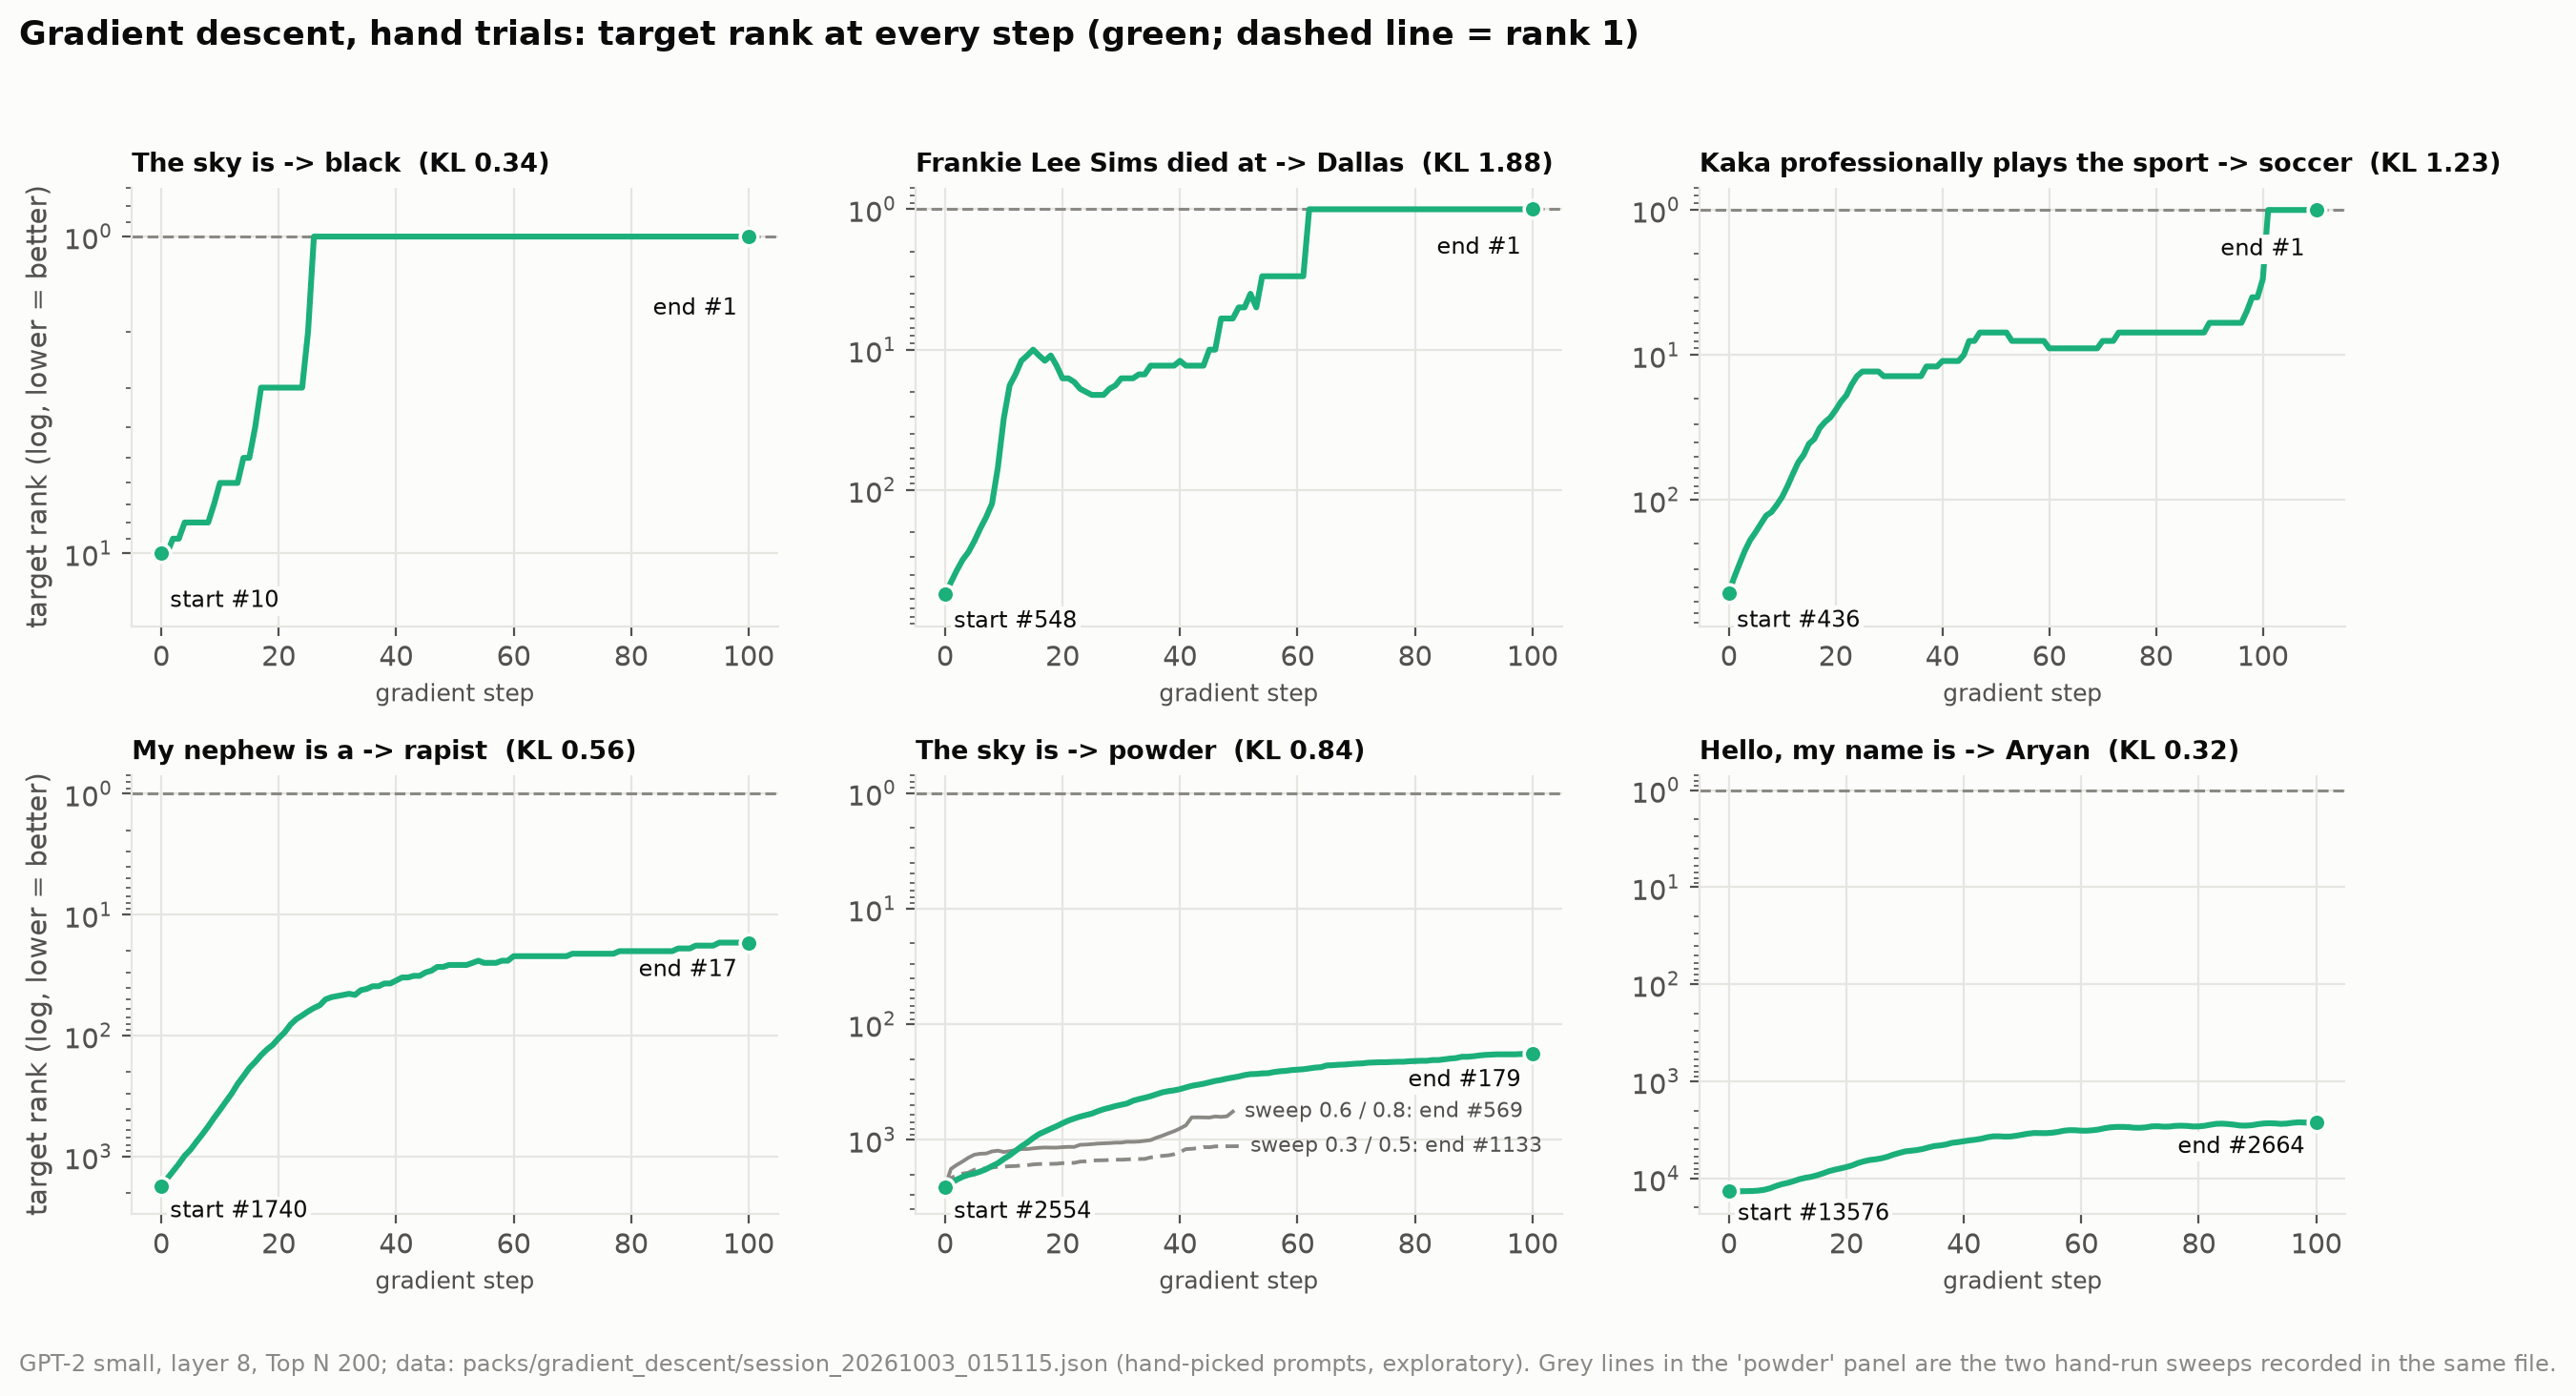
\includegraphics[width=0.97\linewidth]{figures/gd_trials_rank_by_step}
\caption{Target Rank at Every Gradient Step for Six of the Hand Trials (Log Axis, Rank 1 at the Top; the Title of Each Panel Gives the Same-Prompt KL). In the Panel of ``powder'' the Two Grey Lines Are the Two Sweeps Recorded in the Same File (Mute 0.3 / Boost 0.5 Ended at \#1133, Mute 0.6 / Boost 0.8 at \#569). Hand-Picked Prompts, Exploratory}\label{fig:gdtrials}
\end{figure}

\subsection*{B.5 Hand Trials of the Additive Edit}
\addcontentsline{toc}{subsection}{B.5 Hand Trials of the Additive Edit}
Table~\ref{tab:addtrials} gives the first trials of the additive extension (Section~\ref{sec:additive-def}) on six prompts: five that the multiplier edit had failed or distorted in the trials above, and the ``capital of France'' prompt with which the Prototype lab opens. Each cell gives the final rank, the target probability, the same-prompt KL in nats and the edit size as a share of the residual norm at the last position, after 100 steps with $N$ = 200 candidates and, for the additive edit, $M$ = 200 silent candidates, cap factor 1.0 and sparsity weight 0.005. The runs on the ``capital of France'' prompt and the multiplier-only runs that are also in Table~\ref{tab:handtrials} are in the stored session histories. The other additive rows were run by hand during development and were run again on 7 October 2026, for this report, with the same settings (\texttt{tools/\allowbreak{}rerun\_\allowbreak{}additive\_\allowbreak{}hand\_\allowbreak{}trials.\allowbreak{}py}; its output is the file \texttt{hand\_\allowbreak{}trials\_\allowbreak{}rerun\_\allowbreak{}20261007.\allowbreak{}json} in the pack \texttt{docs/\allowbreak{}Research\_\allowbreak{}Journal/\allowbreak{}packs/\allowbreak{}additive\_\allowbreak{}control}); they reproduced the numbers of the research journal in every digit shown.

\begin{table}[H]
\centering
\caption{Hand Trials of the Additive Edit on Six Prompts (Rank, Target Probability, Same-Prompt KL, Edit Size; 100 Steps; Exploratory)}\label{tab:addtrials}
{\small\renewcommand{\arraystretch}{1.15}
\begin{tabular}{|>{\raggedright\arraybackslash}p{0.251\linewidth}|>{\raggedright\arraybackslash}p{0.207\linewidth}|>{\raggedright\arraybackslash}p{0.207\linewidth}|>{\raggedright\arraybackslash}p{0.207\linewidth}|}
\hline
\textbf{Prompt $\rightarrow$ target (start rank)} & \textbf{Multipliers only} & \textbf{Multipliers and additive} & \textbf{Additive, KL charged at every step} \\ \hline
My nephew is a $\rightarrow$ rapist (1740) & \#17, 0.38\%, KL 0.56, 33\% & \textbf{\#1}, 2.27\%, KL 0.20, 57\% & \#1, 2.49\%, KL 0.18, 53\% \\ \hline
The sky is $\rightarrow$ powder (2554) & \#179, 0.08\%, KL 0.84, 38\% & \textbf{\#1}, 8.36\%, KL 0.36, 161\% & \#1, 11.18\%, KL 0.23, 96\% \\ \hline
Hello, my name is $\rightarrow$ Aryan (13576) & \#2664, 0.01\%, KL 0.32, 34\% & \textbf{\#1}, 1.39\%, KL 0.58, 121\% & \#1, 1.20\%, KL 0.24, 55\% \\ \hline
Hello, my name is $\rightarrow$ Rajesh (20214) & \#9231, 0.00\%, KL 0.28, 40\% & \textbf{\#1}, 1.00\%, KL 0.26, 84\% & \#1, 0.99\%, KL 0.17, 79\% \\ \hline
The sky is $\rightarrow$ Adi (14149) & \#4897, 0.00\%, KL 2.71, 57\% & \textbf{\#1}, 8.18\%, KL 0.44, 109\% & \#1, 13.14\%, KL 0.19, 77\% \\ \hline
The capital of France is $\rightarrow$ Hong (3419) & \#1, 1.37\%, KL 4.39, 37\% & \#1, 4.68\%, KL 0.41, 151\% & \#1, 4.24\%, KL 0.20, 78\% \\ \hline
\end{tabular}}
\end{table}

Four points qualify the table. First, the targets are single token pieces: ``Aryan'', ``Rajesh'' and ``Adi'' are words of several tokens and only the last piece is scored (the new top-1 pieces are ``ryan'', ``esh'' and ``i''), and `` Hong'' is only the first piece of ``Hong Kong''; rank 1 here is rank 1 for a piece, not for the word. Second, the additive edits are large: 57\% to 161\% of the residual norm in the third column, whereas free residual pushes of 10 to 20\% of the norm reached rank 1 on 47 to 99\% of the cached prompts in Section~\ref{sec:headroom}. Third, the same-prompt KL is lower with the additive edit than with multipliers alone in five of the six rows (on ``Aryan'' it rose from 0.32 to 0.58) and lower again when the KL is charged at every step in all six. Fourth, an added vector acts on every prompt, because it is added unconditionally at the last position, whereas a multiplier acts only where its feature fires; the controlled measurement of this collateral effect on 20 unrelated prompts is in Table~\ref{tab:reworded}. The additive trials led to the control of Section~\ref{sec:additive}, in which the edit pushed random words to rank 1 on 20 of 20 prompts.

\section*{Appendix C: Code Snippets}
\addcontentsline{toc}{section}{Appendix C: Code Snippets}
The listings below are condensed from the project source to show the core logic; logging, argument validation, device handling and the bookkeeping of the application are omitted. Names follow the source files given in each title.

\begin{lstlisting}[title={Listing C.1: Delta-patching hook with a scale map (hooks.py, condensed)},language=Python]
def make_scale_map_hook(scale_map, sae):
    def hook_fn(resid, hook):                      # resid: [batch, position, d_model]; every position
        acts = sae.encode(resid)                   # sparse feature activations
        base = sae.decode(acts)                    # reconstruction of the unedited features
        edited = acts.clone()
        idx = torch.as_tensor(list(scale_map.keys()), device=resid.device)
        mult = torch.as_tensor(list(scale_map.values()), device=resid.device, dtype=acts.dtype)
        edited[..., idx] = edited[..., idx] * mult # mute: m < 1 (0 removes), boost: m > 1
        # delta patch: only the change is added, so the reconstruction error stays untouched
        return resid + (sae.decode(edited) - base)
    return hook_fn
\end{lstlisting}

\begin{lstlisting}[title={Listing C.2: Two-stage causal ranking of the candidate features (editing.py, condensed)},language=Python]
def get_top_competitor_features(model, sae, prompt, current_top_token_id, top_n=20, clean_ctx=None,
                                use_batched=False, exclude_ids=None, base_scale_map=None, positions="last"):
    tokens = clean_ctx.tokens
    p_clean = clean_ctx.clean_probs[current_top_token_id].item()
    # Stage 1: the top_n most active features (last token, or the maximum over all prompt positions)
    active = get_top_active_features(model, sae, prompt, top_n, clean_ctx, exclude_ids, positions)
    ids = [fid for fid, _ in active]
    # Stage 2: remove each candidate alone (scale 0), all candidates in GPU batches, and read the competitor's probability
    p_ablated = batched_ablation_probs(model, sae, tokens, ids, scale=0.0,
                                       token_ids_of_interest=[current_top_token_id],
                                       hook_name=hook_name, base_scale_map=base_scale_map)[:, 0]
    results = [(fid, p - p_clean) for fid, p in zip(ids, p_ablated.tolist())]
    return sorted(results, key=lambda t: t[1])     # most negative first: the largest drop of the competitor
\end{lstlisting}

\begin{lstlisting}[title={Listing C.3: Eligibility classification (evaluation.py, condensed)},language=Python]
def classify_fact(model, prompt, target_str):
    target_token_id = get_target_token_id(model, target_str)
    probs = model(model.to_tokens(prompt))[0, -1].softmax(-1)
    clean_prob = probs[target_token_id].item()
    rank = int((probs > probs[target_token_id]).sum()) + 1
    if rank == 1:
        label = "already_correct"
    elif clean_prob > 0.01 or rank <= 50:          # either condition is enough
        label = "suppressed"
    else:
        label = "absent"
    return {"clean_prob": clean_prob, "rank": rank, "label": label}
\end{lstlisting}

\begin{lstlisting}[title={Listing C.4: Gradient-descent editor, one multiplier per candidate feature (gradient_editing.py, condensed)},language=Python]
BETA_MAX = 2.0
Z_ZERO = -math.log(BETA_MAX)                       # sigmoid(Z_ZERO) = 1/3, so a = 0 (no edit) at the start

def to_a(z):                                       # multiplier m = 1 + a lies in (0, 3)
    return -1.0 + (1.0 + BETA_MAX) * torch.sigmoid(z)

def edit_by_gradient_descent(resid, acts, W_dec, clean_last, target_id, blocker_id,
                             steps=100, lr=0.1, lam_kl=3.0, lam_size=0.005, margin_target=0.3):
    # acts: [position, K] activations of the K candidates; W_dec: [K, d_model] their decoder directions
    amax = acts.max(dim=0).values
    w = amax / amax.sum()                          # size penalty weighted by how loud each feature is
    z = torch.full((acts.shape[1],), Z_ZERO, requires_grad=True)
    opt = torch.optim.Adam([z], lr=lr)
    best_key, best_a = float("inf"), None
    for step in range(steps + 1):
        a = to_a(z)
        delta = torch.einsum("pk,k,kd->pd", acts, a, W_dec)   # delta patch at every position
        last = last_logits(resid + delta)          # only blocks layer..11 are recomputed
        rank, prob, kl, margin = score(last, clean_last, target_id, blocker_id)
        lead = float(margin >= margin_target)      # the KL term is switched on once the target leads
        loss = relu(margin_target - margin) + lam_kl * kl * lead + lam_size * (a.abs() * w).sum()
        key = (1e6 if rank > 1 else 0.0) + loss.item()        # keep the best iterate, not the last
        if key < best_key:
            best_key, best_a = key, a.detach().clone()
        if step == steps:
            break
        z.grad = torch.autograd.grad(loss, [z])[0]            # gradient with respect to z only
        opt.step()
    return best_a           # re-checked afterwards through the real hook (Listing C.1)
\end{lstlisting}

\begin{lstlisting}[title={Listing C.5: Hook with multipliers and additive amounts (hooks.py, condensed)},language=Python]
def make_scale_and_add_hook(scale_map, add_map, sae):
    scale_hook = make_scale_map_hook(scale_map, sae)
    def hook_fn(resid, hook):
        out = scale_hook(resid, hook).clone()
        if add_map:                                # silent features switched on at the LAST position only
            ids = torch.as_tensor(list(add_map.keys()), device=resid.device)
            amounts = torch.as_tensor(list(add_map.values()), device=resid.device, dtype=resid.dtype)
            out[:, -1, :] = out[:, -1, :] + amounts @ sae.W_dec[ids].to(resid.dtype)
        return out
    return hook_fn
\end{lstlisting}

\section*{Appendix D: Reproducing the Results}
\addcontentsline{toc}{section}{Appendix D: Reproducing the Results}
\setcounter{table}{0}\renewcommand{\thetable}{D.\arabic{table}}\renewcommand{\theHtable}{D.\arabic{table}}
All code, the stored data packs and the research journal (entries 1 to 30, one per experiment) are in the project repository, \url{https://github.com/adi5022/Mechanistic-Intervention-of-Large-Language-Models-via-Sparse-AutoEncoders}, branch \texttt{gradient-descent-editing}. \todo{confirm that the repository is public, or state how examiners can obtain the code}

\subsection*{D.1 Environment and Data}
\addcontentsline{toc}{subsection}{D.1 Environment and Data}
The software versions used for the reported results are those of Table~\ref{tab:environment}. Commands below are written for the Windows PC, as \texttt{.\allowbreak{}venv\textbackslash{}Scripts\textbackslash{}python.\allowbreak{}exe tools/\allowbreak{}.\allowbreak{}.\allowbreak{}.\allowbreak{}}; on macOS the interpreter is \texttt{.\allowbreak{}venv/\allowbreak{}bin/\allowbreak{}python}. The code chooses the device in the order CUDA, MPS, CPU; the environment variable \texttt{FEATURESCALPEL\_\allowbreak{}DEVICE}, set to \texttt{cpu}, \texttt{mps} or \texttt{cuda}, overrides the choice.

\begin{lstlisting}[title={Listing D.1: Setting up the environment and the data}]
# Windows, NVIDIA GPU
python -m venv .venv
.venv\Scripts\python.exe -m pip install -r requirements.txt
.venv\Scripts\streamlit.exe run experiment_app.py          # the application, http://localhost:8501

# macOS, Apple silicon
bash scripts/setup_mac.sh                                  # environment from mac_requirements.txt
bash scripts/get_data_mac.sh                               # CounterFact download and hard-set build
bash scripts/run_app_mac.sh                                # the application
\end{lstlisting}

Some data are not stored in the repository and have to be rebuilt: the CounterFact file \texttt{datasets/\allowbreak{}counterfact.\allowbreak{}json} (about 45 MB, downloaded from the data site of the ROME project; its checksum is recorded in \texttt{scripts/\allowbreak{}get\_\allowbreak{}data\_\allowbreak{}mac.\allowbreak{}sh}); the hard set \texttt{data/\allowbreak{}counterfact\_\allowbreak{}hard\_\allowbreak{}set.\allowbreak{}json}, built from it by \texttt{tools/\allowbreak{}build\_\allowbreak{}counterfact\_\allowbreak{}set.\allowbreak{}py}; and the per-prompt cache and tables of the learned-strength study (\texttt{outputs/\allowbreak{}strength\_\allowbreak{}cache} and \texttt{outputs/\allowbreak{}strength\_\allowbreak{}tables}), which are needed only to repeat Sections~\ref{sec:headroom} and~\ref{sec:learned}. The split of the hard set (\texttt{data/\allowbreak{}counterfact\_\allowbreak{}split.\allowbreak{}json}) and the packs with the results of every study (\texttt{docs/\allowbreak{}Research\_\allowbreak{}Journal/\allowbreak{}packs/\allowbreak{}}) are in the repository. The application and the Prototype lab need only the model and the SAE, which are downloaded from the Hugging Face Hub on first use.

\subsection*{D.2 Commands for Each Study}
\addcontentsline{toc}{subsection}{D.2 Commands for Each Study}
Table~\ref{tab:repro} lists the command of each study, where it writes its output, and the run time where one was recorded. A run time belongs to the machine named and must not be compared with one from another machine.

{\small\renewcommand{\arraystretch}{1.15}
\begin{longtable}{|>{\raggedright\arraybackslash}p{0.148\linewidth}|>{\raggedright\arraybackslash}p{0.340\linewidth}|>{\raggedright\arraybackslash}p{0.222\linewidth}|>{\raggedright\arraybackslash}p{0.163\linewidth}|}
\caption{Commands, Outputs and Recorded Run Times of the Studies}\label{tab:repro}\\
\hline
\textbf{Study (section)} & \textbf{Command} & \textbf{Output} & \textbf{Recorded run time} \\ \hline
\endfirsthead
\hline
\textbf{Study (section)} & \textbf{Command} & \textbf{Output} & \textbf{Recorded run time} \\ \hline
\endhead
Hard set and split (\ref{sec:data}) & \texttt{tools/\allowbreak{}build\_\allowbreak{}counterfact\_\allowbreak{}set.\allowbreak{}py}, then \texttt{tools/\allowbreak{}split\_\allowbreak{}counterfact\_\allowbreak{}set.\allowbreak{}py} & \texttt{data/\allowbreak{}counterfact\_\allowbreak{}hard\_\allowbreak{}set.\allowbreak{}json}, \texttt{data/\allowbreak{}counterfact\_\allowbreak{}split.\allowbreak{}json} & not recorded \\ \hline
Candidate source (\ref{sec:candsrc}) & \texttt{run\_\allowbreak{}batch.\allowbreak{}py data/\allowbreak{}candidate\_\allowbreak{}source\_\allowbreak{}batch\_\allowbreak{}spec.\allowbreak{}json outputs/\allowbreak{}batch\_\allowbreak{}runs/\allowbreak{}repro.\allowbreak{}json} & the file named; the original run is in \texttt{benchmark\_\allowbreak{}results/\allowbreak{}candidate\_\allowbreak{}source\_\allowbreak{}study} & about 5 minutes on a CUDA GPU \\ \hline
Safety filter (\ref{sec:filter}) & \texttt{run\_\allowbreak{}batch.\allowbreak{}py data/\allowbreak{}safety\_\allowbreak{}filter\_\allowbreak{}spec\_\allowbreak{}pilot.\allowbreak{}json outputs/\allowbreak{}safety\_\allowbreak{}batches/\allowbreak{}safety\_\allowbreak{}filter\_\allowbreak{}spec\_\allowbreak{}pilot.\allowbreak{}json}, and the same with \texttt{safety\_\allowbreak{}filter\_\allowbreak{}spec\_\allowbreak{}full\_\allowbreak{}last.\allowbreak{}json}; then \texttt{tools/\allowbreak{}analyze\_\allowbreak{}safety\_\allowbreak{}batch.\allowbreak{}py} on the result file & \texttt{outputs/\allowbreak{}safety\_\allowbreak{}batches/\allowbreak{}}; packs \texttt{docs/\allowbreak{}Research\_\allowbreak{}Journal/\allowbreak{}packs/\allowbreak{}entry21\_\allowbreak{}*} & not recorded \\ \hline
Repair and SAE limit (\ref{sec:repair}) & \texttt{tools/\allowbreak{}run\_\allowbreak{}repair\_\allowbreak{}diagnostics.\allowbreak{}py} & \texttt{outputs/\allowbreak{}repair\_\allowbreak{}diagnostics/\allowbreak{}repair\_\allowbreak{}run.\allowbreak{}json} & about 2.5 to 3 minutes per prompt and layer (GTX 1660 Ti, shared) \\ \hline
Cache, headroom, tables (\ref{sec:headroom}, \ref{sec:learned}) & \texttt{tools/\allowbreak{}build\_\allowbreak{}strength\_\allowbreak{}cache.\allowbreak{}py}, \texttt{tools/\allowbreak{}measure\_\allowbreak{}headroom.\allowbreak{}py}, \texttt{tools/\allowbreak{}build\_\allowbreak{}strength\_\allowbreak{}tables.\allowbreak{}py} & \texttt{outputs/\allowbreak{}strength\_\allowbreak{}cache}, \texttt{outputs/\allowbreak{}headroom}, \texttt{outputs/\allowbreak{}strength\_\allowbreak{}tables} & tables for 1,450 prompts: 49 minutes (RTX 4050 laptop), about 1.9 hours (GTX 1660 Ti); headroom: 1,060 s (RTX 4050 laptop) \\ \hline
Learned strengths (\ref{sec:learned}) & \texttt{tools/\allowbreak{}train\_\allowbreak{}strength\_\allowbreak{}models.\allowbreak{}py}, then \texttt{tools/\allowbreak{}analyse\_\allowbreak{}strength\_\allowbreak{}models.\allowbreak{}py --dir outputs/\allowbreak{}strength\_\allowbreak{}models/\allowbreak{}<time>} & \texttt{outputs/\allowbreak{}strength\_\allowbreak{}models/\allowbreak{}<time>}; pack \texttt{docs/\allowbreak{}Research\_\allowbreak{}Journal/\allowbreak{}packs/\allowbreak{}strength\_\allowbreak{}models} & trained on the RTX 4050 laptop; time not recorded \\ \hline
Gradient descent against the sweeps (\ref{sec:gdvs}) & \texttt{tools/\allowbreak{}compare\_\allowbreak{}sweep\_\allowbreak{}vs\_\allowbreak{}gradient.\allowbreak{}py --n-per-band 0} (all 300 prompts; \texttt{--resume --out <folder>} continues a stopped run) & \texttt{outputs/\allowbreak{}sweep\_\allowbreak{}vs\_\allowbreak{}gradient/\allowbreak{}<time>}; pack \texttt{docs/\allowbreak{}Research\_\allowbreak{}Journal/\allowbreak{}packs/\allowbreak{}sweep\_\allowbreak{}vs\_\allowbreak{}gradient} & about 9 hours (GTX 1660 Ti) \\ \hline
Self-checks of the additive edit (\ref{sec:additive}) & \texttt{tools/\allowbreak{}check\_\allowbreak{}additive.\allowbreak{}py} & console & not recorded \\ \hline
Random-word control (\ref{sec:additive}) & \texttt{tools/\allowbreak{}control\_\allowbreak{}random\_\allowbreak{}targets.\allowbreak{}py} & \texttt{docs/\allowbreak{}Research\_\allowbreak{}Journal/\allowbreak{}packs/\allowbreak{}additive\_\allowbreak{}control/\allowbreak{}results.\allowbreak{}json} & not recorded \\ \hline
Hand trials of the additive edit (Appendix B.5) & \texttt{tools/\allowbreak{}rerun\_\allowbreak{}additive\_\allowbreak{}hand\_\allowbreak{}trials.\allowbreak{}py} & \texttt{docs/\allowbreak{}Research\_\allowbreak{}Journal/\allowbreak{}packs/\allowbreak{}additive\_\allowbreak{}control/\allowbreak{}hand\_\allowbreak{}trials\_\allowbreak{}rerun\_\allowbreak{}20261007.\allowbreak{}json} & about 8.5 seconds per edit (GTX 1660 Ti), 18 edits \\ \hline
Reworded prompts (\ref{sec:additive}) & \texttt{tools/\allowbreak{}test\_\allowbreak{}generalisation.\allowbreak{}py --targets true}, and with \texttt{--targets random} & \texttt{outputs/\allowbreak{}generalisation/\allowbreak{}<time>}; packs \texttt{docs/\allowbreak{}Research\_\allowbreak{}Journal/\allowbreak{}packs/\allowbreak{}generalisation} & not recorded \\ \hline
Generated text and instructions (\ref{sec:beyond}) & \texttt{tools/\allowbreak{}test\_\allowbreak{}generation\_\allowbreak{}quality.\allowbreak{}py --n-per-band 10} & \texttt{outputs/\allowbreak{}generation\_\allowbreak{}quality/\allowbreak{}<time>}; pack \texttt{docs/\allowbreak{}Research\_\allowbreak{}Journal/\allowbreak{}packs/\allowbreak{}generation\_\allowbreak{}quality} & not recorded \\ \hline
Figures of this report & \texttt{tools/\allowbreak{}make\_\allowbreak{}report\_\allowbreak{}figures.\allowbreak{}py --out figures} & the figure files \texttt{fig\_\allowbreak{}*.\allowbreak{}png} and \texttt{gd\_\allowbreak{}*.\allowbreak{}png}, and \texttt{report\_\allowbreak{}figure\_\allowbreak{}data.\allowbreak{}json} with every plotted number & not recorded \\ \hline
Mac parity check & \texttt{tools/\allowbreak{}check\_\allowbreak{}mac\_\allowbreak{}parity.\allowbreak{}py} (\texttt{--full} adds the additive self-checks) & console & not recorded \\ \hline
\end{longtable}}

The three tools that compare methods on the held-out prompts (\texttt{compare\_\allowbreak{}sweep\_\allowbreak{}vs\_\allowbreak{}gradient.\allowbreak{}py}, \texttt{test\_\allowbreak{}generalisation.\allowbreak{}py} and \texttt{test\_\allowbreak{}generation\_\allowbreak{}quality.\allowbreak{}py}) write a \texttt{meta.\allowbreak{}json} with their arguments next to their results, choose their prompts with a seeded generator (seed 7 unless changed) and can be resumed. The hand trials of Appendix~B were made in the application (Hybrid tab and Prototype lab) and are saved in its session history (\texttt{outputs/\allowbreak{}session\_\allowbreak{}history/\allowbreak{}}); the file of the first set of trials is in the pack \texttt{docs/\allowbreak{}Research\_\allowbreak{}Journal/\allowbreak{}packs/\allowbreak{}gradient\_\allowbreak{}descent}.

\section*{Appendix E: Where Each Result Comes From}
\addcontentsline{toc}{section}{Appendix E: Where Each Result Comes From}
\setcounter{table}{0}\renewcommand{\thetable}{E.\arabic{table}}\renewcommand{\theHtable}{E.\arabic{table}}
Table~\ref{tab:evidence} lists, for each result of Chapter~\ref{ch:results-and-discussion}, where the data behind it is stored in the repository and what kind of measurement it is. \textit{Real model} means that the edit was applied through the real hook on GPT-2 small and the rank was read from the real output. \textit{Stand-in} means a cheaper substitute for the real sweep (the cached-state push of Section~\ref{sec:headroom} or the prefix proxy of Section~\ref{sec:learned}), whose numbers are not rates of the real sweep. \textit{Hand-picked} means prompts chosen by the authors, which show that something can happen but not how often. Journal entries are the files \texttt{docs/\allowbreak{}Research\_\allowbreak{}Journal/\allowbreak{}N.\allowbreak{}md}, and packs are the folders \texttt{docs/\allowbreak{}Research\_\allowbreak{}Journal/\allowbreak{}packs/\allowbreak{}}.

{\small\renewcommand{\arraystretch}{1.15}
\begin{longtable}{|>{\raggedright\arraybackslash}p{0.277\linewidth}|>{\raggedright\arraybackslash}p{0.090\linewidth}|>{\raggedright\arraybackslash}p{0.294\linewidth}|>{\raggedright\arraybackslash}p{0.212\linewidth}|}
\caption{Evidence Behind the Results of Chapter 5}\label{tab:evidence}\\
\hline
\textbf{Result} & \textbf{Section} & \textbf{Stored evidence} & \textbf{Kind of measurement} \\ \hline
\endfirsthead
\hline
\textbf{Result} & \textbf{Section} & \textbf{Stored evidence} & \textbf{Kind of measurement} \\ \hline
\endhead
Eligibility of the 45 ROME facts (15 already correct, 22 suppressed, 8 low prior) & \ref{sec:data} & \texttt{src/\allowbreak{}fact\_\allowbreak{}bank.\allowbreak{}py}, \texttt{src/\allowbreak{}evaluation.\allowbreak{}py}; journal entry 1 & real model, 45 facts \\ \hline
Competitor ablation reached rank 1 on 3 of 22 facts, target-helper ablation on 1 of 22 & \ref{sec:dev-results} & journal entries 2 and 3; Appendix B.3 & real model, 22 suppressed facts, one run each \\ \hline
Weighted reduction, decay profiles, Top-K muting and the hybrid mute and boost during development & \ref{sec:dev-results} & journal entries 4 to 8 & real model, one prompt or a few prompts \\ \hline
Depth of the intervention (layer 8 largest mean gain) & \ref{sec:depth} & journal entry 10; \texttt{benchmark\_\allowbreak{}results/\allowbreak{}layer\_\allowbreak{}benchmark\_\allowbreak{}*.\allowbreak{}json} & real model, 21 prompts at 12 layers (12 with room to improve) \\ \hline
Cost of the sweep and of its optimisations (186, 126 and 6 forward calls; GPU against CPU; stage profile) & \ref{sec:cost} & journal entries 11 to 15; \texttt{benchmark\_\allowbreak{}results/\allowbreak{}}, \texttt{benchmark\_\allowbreak{}results\_\allowbreak{}audit/\allowbreak{}} & real model, one prompt for the call counts, 21 prompts for the profile \\ \hline
Candidate source: all positions 10 of 13 against last token 4 of 13 & \ref{sec:candsrc} & journal entry 20; \texttt{benchmark\_\allowbreak{}results/\allowbreak{}candidate\_\allowbreak{}source\_\allowbreak{}study}; \texttt{data/\allowbreak{}candidate\_\allowbreak{}source\_\allowbreak{}batch\_\allowbreak{}spec.\allowbreak{}json} & real model, 13 steerable prompts of 17, paired \\ \hline
Safety filter: 29 against 19 of 45, and 41 against 35 of 131 & \ref{sec:filter} & journal entry 21 (numbers recorded, interpretation not written); packs \texttt{entry21\_\allowbreak{}pilot\_\allowbreak{}20260926\_\allowbreak{}1812} and \texttt{entry21\_\allowbreak{}full\_\allowbreak{}last\_\allowbreak{}20260926\_\allowbreak{}1840} & real model, 45 and 131 prompts \\ \hline
Repair and SAE limit (pushed direction persists at 0.79 to 1.29; SAE-free edit reaches rank 1 in 21 of 21 combinations, the SAE edit in 1 of 21) & \ref{sec:repair} & journal entry 22; pack \texttt{repair\_\allowbreak{}diagnostics} & real model, three hand-picked prompts on which the sweep had failed, layers 5 to 11 \\ \hline
Headroom of feature scaling (80\% and 41\%) & \ref{sec:headroom} & journal entries 23 and 24; pack \texttt{headroom/\allowbreak{}headroom\_\allowbreak{}20261002\_\allowbreak{}144917.\allowbreak{}json} & stand-in, 1,450 prompts \\ \hline
Learned strengths (75, 116, 119, 123 of 300) & \ref{sec:learned} & journal entries 26 and 27; pack \texttt{strength\_\allowbreak{}models} & stand-in (prefix proxy), 300 held-out prompts \\ \hline
Gradient descent against the sweeps (271, 161 and 94 of 300) & \ref{sec:gdvs} & journal entry 29; pack \texttt{sweep\_\allowbreak{}vs\_\allowbreak{}gradient} (\texttt{runs.\allowbreak{}jsonl}, \texttt{summary.\allowbreak{}json}) & real model, 300 held-out prompts, paired \\ \hline
Hand trials of gradient descent and of the additive edit & Appendix B.4, B.5 & journal entries 28 and 30; pack \texttt{gradient\_\allowbreak{}descent}; for B.5 also \texttt{additive\_\allowbreak{}control/\allowbreak{}hand\_\allowbreak{}trials\_\allowbreak{}rerun\_\allowbreak{}20261007.\allowbreak{}json} & hand-picked, 9 and 6 prompts \\ \hline
Random-word control of the additive edit (20 of 20) & \ref{sec:additive} & journal entry 30, section 10; pack \texttt{additive\_\allowbreak{}control/\allowbreak{}results.\allowbreak{}json} & real model, 20 validation prompts \\ \hline
Reworded, neighbouring and unrelated prompts & \ref{sec:additive} & journal entry 30, section 11; packs \texttt{generalisation/\allowbreak{}true40} and \texttt{random40} & real model, 40 test prompts, true and random targets \\ \hline
Generated text and the do-not-say instruction & \ref{sec:beyond} & journal entry 30, section 15; pack \texttt{generation\_\allowbreak{}quality/\allowbreak{}true40} & real model, 40 test prompts, greedy decoding of 20 tokens \\ \hline
Thread race on the start-of-text token (16 of 57 recorded runs affected) & \ref{sec:lessons} & journal entry 30, section 13 & the application's own run records \\ \hline
Parity of the macOS port & \ref{sec:checks} & \texttt{tools/\allowbreak{}check\_\allowbreak{}mac\_\allowbreak{}parity.\allowbreak{}py}; \texttt{docs/\allowbreak{}handoff\_\allowbreak{}2026-10-05\_\allowbreak{}mac.\allowbreak{}md} & not measured on MPS; CPU path checked on the Windows PC \\ \hline
The data figures of Chapters 3 and 5 & Chapters 3 and 5 & \texttt{tools/\allowbreak{}make\_\allowbreak{}report\_\allowbreak{}figures.\allowbreak{}py}; \texttt{report\_\allowbreak{}figure\_\allowbreak{}data.\allowbreak{}json} lists every plotted number & stored data of the rows above (the architecture, flow and layout diagrams are schematics) \\ \hline
\end{longtable}}

\end{document}
